\documentclass[twoside]{book}

% Packages required by doxygen
\usepackage{fixltx2e}
\usepackage{calc}
\usepackage{doxygen}
\usepackage{graphicx}
\usepackage[utf8]{inputenc}
\usepackage{makeidx}
\usepackage{multicol}
\usepackage{multirow}
\PassOptionsToPackage{warn}{textcomp}
\usepackage{textcomp}
\usepackage[nointegrals]{wasysym}
\usepackage[table]{xcolor}

% Font selection
\usepackage[T1]{fontenc}
\usepackage{mathptmx}
\usepackage[scaled=.90]{helvet}
\usepackage{courier}
\usepackage{amssymb}
\usepackage{sectsty}
\renewcommand{\familydefault}{\sfdefault}
\allsectionsfont{%
  \fontseries{bc}\selectfont%
  \color{darkgray}%
}
\renewcommand{\DoxyLabelFont}{%
  \fontseries{bc}\selectfont%
  \color{darkgray}%
}
\newcommand{\+}{\discretionary{\mbox{\scriptsize$\hookleftarrow$}}{}{}}

% Page & text layout
\usepackage{geometry}
\geometry{%
  a4paper,%
  top=2.5cm,%
  bottom=2.5cm,%
  left=2.5cm,%
  right=2.5cm%
}
\tolerance=750
\hfuzz=15pt
\hbadness=750
\setlength{\emergencystretch}{15pt}
\setlength{\parindent}{0cm}
\setlength{\parskip}{0.2cm}
\makeatletter
\renewcommand{\paragraph}{%
  \@startsection{paragraph}{4}{0ex}{-1.0ex}{1.0ex}{%
    \normalfont\normalsize\bfseries\SS@parafont%
  }%
}
\renewcommand{\subparagraph}{%
  \@startsection{subparagraph}{5}{0ex}{-1.0ex}{1.0ex}{%
    \normalfont\normalsize\bfseries\SS@subparafont%
  }%
}
\makeatother

% Headers & footers
\usepackage{fancyhdr}
\pagestyle{fancyplain}
\fancyhead[LE]{\fancyplain{}{\bfseries\thepage}}
\fancyhead[CE]{\fancyplain{}{}}
\fancyhead[RE]{\fancyplain{}{\bfseries\leftmark}}
\fancyhead[LO]{\fancyplain{}{\bfseries\rightmark}}
\fancyhead[CO]{\fancyplain{}{}}
\fancyhead[RO]{\fancyplain{}{\bfseries\thepage}}
\fancyfoot[LE]{\fancyplain{}{}}
\fancyfoot[CE]{\fancyplain{}{}}
\fancyfoot[RE]{\fancyplain{}{\bfseries\scriptsize Generated on Mon Sep 14 2015 19\+:04\+:51 for P\+F\+Q C++ library by Doxygen }}
\fancyfoot[LO]{\fancyplain{}{\bfseries\scriptsize Generated on Mon Sep 14 2015 19\+:04\+:51 for P\+F\+Q C++ library by Doxygen }}
\fancyfoot[CO]{\fancyplain{}{}}
\fancyfoot[RO]{\fancyplain{}{}}
\renewcommand{\footrulewidth}{0.4pt}
\renewcommand{\chaptermark}[1]{%
  \markboth{#1}{}%
}
\renewcommand{\sectionmark}[1]{%
  \markright{\thesection\ #1}%
}

% Indices & bibliography
\usepackage{natbib}
\usepackage[titles]{tocloft}
\setcounter{tocdepth}{3}
\setcounter{secnumdepth}{5}
\makeindex

% Hyperlinks (required, but should be loaded last)
\usepackage{ifpdf}
\ifpdf
  \usepackage[pdftex,pagebackref=true]{hyperref}
\else
  \usepackage[ps2pdf,pagebackref=true]{hyperref}
\fi
\hypersetup{%
  colorlinks=true,%
  linkcolor=blue,%
  citecolor=blue,%
  unicode%
}

% Custom commands
\newcommand{\clearemptydoublepage}{%
  \newpage{\pagestyle{empty}\cleardoublepage}%
}


%===== C O N T E N T S =====

\begin{document}

% Titlepage & ToC
\hypersetup{pageanchor=false,
             bookmarks=true,
             bookmarksnumbered=true,
             pdfencoding=unicode
            }
\pagenumbering{roman}
\begin{titlepage}
\vspace*{7cm}
\begin{center}%
{\Large P\+F\+Q C++ library \\[1ex]\large v5.\+1 }\\
\vspace*{1cm}
{\large Generated by Doxygen 1.8.8}\\
\vspace*{0.5cm}
{\small Mon Sep 14 2015 19:04:51}\\
\end{center}
\end{titlepage}
\clearemptydoublepage
\tableofcontents
\clearemptydoublepage
\pagenumbering{arabic}
\hypersetup{pageanchor=true}

%--- Begin generated contents ---
\chapter{Namespace Index}
\section{Namespace List}
Here is a list of all namespaces with brief descriptions\+:\begin{DoxyCompactList}
\item\contentsline{section}{\hyperlink{namespacepfq__lang}{pfq\+\_\+lang} }{\pageref{namespacepfq__lang}}{}
\item\contentsline{section}{\hyperlink{namespacepfq__lang_1_1anonymous__namespace_02default_8hpp_03}{pfq\+\_\+lang\+::anonymous\+\_\+namespace\{default.\+hpp\}} }{\pageref{namespacepfq__lang_1_1anonymous__namespace_02default_8hpp_03}}{}
\item\contentsline{section}{\hyperlink{namespacepfq__lang_1_1term}{pfq\+\_\+lang\+::term} }{\pageref{namespacepfq__lang_1_1term}}{}
\end{DoxyCompactList}

\chapter{Hierarchical Index}
\section{Class Hierarchy}
This inheritance list is sorted roughly, but not completely, alphabetically\+:\begin{DoxyCompactList}
\item \contentsline{section}{pfq\+:\+:lang\+:\+:Action$<$ a $>$}{\pageref{structpfq_1_1lang_1_1Action}}{}
\item \contentsline{section}{pfq\+:\+:lang\+:\+:Argument}{\pageref{structpfq_1_1lang_1_1Argument}}{}
\item bool\+\_\+type\begin{DoxyCompactList}
\item \contentsline{section}{pfq\+:\+:lang\+:\+:has\+\_\+insertion\+\_\+operator$<$ T $>$}{\pageref{structpfq_1_1lang_1_1has__insertion__operator}}{}
\item \contentsline{section}{pfq\+:\+:lang\+:\+:is\+\_\+mfunction$<$ Tp $>$}{\pageref{structpfq_1_1lang_1_1is__mfunction}}{}
\item \contentsline{section}{pfq\+:\+:lang\+:\+:is\+\_\+predicate$<$ Tp $>$}{\pageref{structpfq_1_1lang_1_1is__predicate}}{}
\item \contentsline{section}{pfq\+:\+:lang\+:\+:is\+\_\+property$<$ Tp $>$}{\pageref{structpfq_1_1lang_1_1is__property}}{}
\end{DoxyCompactList}
\item \contentsline{section}{pfq\+:\+:lang\+:\+:Composition$<$ F, G $>$}{\pageref{structpfq_1_1lang_1_1Composition}}{}
\item false\+\_\+type\begin{DoxyCompactList}
\item \contentsline{section}{pfq\+:\+:lang\+:\+:is\+\_\+\+Function$<$ Tp $>$}{\pageref{structpfq_1_1lang_1_1is__Function}}{}
\item \contentsline{section}{pfq\+:\+:lang\+:\+:is\+\_\+same\+\_\+type\+\_\+constructor$<$ T, Tp $>$}{\pageref{structpfq_1_1lang_1_1is__same__type__constructor}}{}
\end{DoxyCompactList}
\item \contentsline{section}{pfq\+:\+:lang\+:\+:Function$<$ Sig $>$}{\pageref{structpfq_1_1lang_1_1Function}}{}
\begin{DoxyCompactList}
\item \contentsline{section}{pfq\+:\+:lang\+:\+:Combinator1$<$ Pred $>$}{\pageref{structpfq_1_1lang_1_1Combinator1}}{}
\item \contentsline{section}{pfq\+:\+:lang\+:\+:Combinator2$<$ Pred1, Pred2 $>$}{\pageref{structpfq_1_1lang_1_1Combinator2}}{}
\item \contentsline{section}{pfq\+:\+:lang\+:\+:M\+Function}{\pageref{structpfq_1_1lang_1_1MFunction}}{}
\item \contentsline{section}{pfq\+:\+:lang\+:\+:M\+Function1}{\pageref{structpfq_1_1lang_1_1MFunction1}}{}
\item \contentsline{section}{pfq\+:\+:lang\+:\+:M\+Function1\+P$<$ P $>$}{\pageref{structpfq_1_1lang_1_1MFunction1P}}{}
\item \contentsline{section}{pfq\+:\+:lang\+:\+:M\+Function2}{\pageref{structpfq_1_1lang_1_1MFunction2}}{}
\item \contentsline{section}{pfq\+:\+:lang\+:\+:M\+Function3}{\pageref{structpfq_1_1lang_1_1MFunction3}}{}
\item \contentsline{section}{pfq\+:\+:lang\+:\+:M\+Function\+F$<$ F $>$}{\pageref{structpfq_1_1lang_1_1MFunctionF}}{}
\item \contentsline{section}{pfq\+:\+:lang\+:\+:M\+Function\+F\+F$<$ F, G $>$}{\pageref{structpfq_1_1lang_1_1MFunctionFF}}{}
\item \contentsline{section}{pfq\+:\+:lang\+:\+:M\+Function\+P$<$ P $>$}{\pageref{structpfq_1_1lang_1_1MFunctionP}}{}
\item \contentsline{section}{pfq\+:\+:lang\+:\+:M\+Function\+P\+F$<$ P, F $>$}{\pageref{structpfq_1_1lang_1_1MFunctionPF}}{}
\item \contentsline{section}{pfq\+:\+:lang\+:\+:M\+Function\+P\+F\+F$<$ P, F, G $>$}{\pageref{structpfq_1_1lang_1_1MFunctionPFF}}{}
\item \contentsline{section}{pfq\+:\+:lang\+:\+:Predicate}{\pageref{structpfq_1_1lang_1_1Predicate}}{}
\item \contentsline{section}{pfq\+:\+:lang\+:\+:Predicate1}{\pageref{structpfq_1_1lang_1_1Predicate1}}{}
\item \contentsline{section}{pfq\+:\+:lang\+:\+:Predicate2}{\pageref{structpfq_1_1lang_1_1Predicate2}}{}
\item \contentsline{section}{pfq\+:\+:lang\+:\+:Predicate3}{\pageref{structpfq_1_1lang_1_1Predicate3}}{}
\item \contentsline{section}{pfq\+:\+:lang\+:\+:Predicate\+R$<$ Prop $>$}{\pageref{structpfq_1_1lang_1_1PredicateR}}{}
\item \contentsline{section}{pfq\+:\+:lang\+:\+:Predicate\+R1$<$ Prop $>$}{\pageref{structpfq_1_1lang_1_1PredicateR1}}{}
\item \contentsline{section}{pfq\+:\+:lang\+:\+:Property}{\pageref{structpfq_1_1lang_1_1Property}}{}
\end{DoxyCompactList}
\item \contentsline{section}{pfq\+:\+:lang\+:\+:Function\+Descr}{\pageref{structpfq_1_1lang_1_1FunctionDescr}}{}
\item \contentsline{section}{pfq\+:\+:lang\+:\+:ipv4\+\_\+t}{\pageref{structpfq_1_1lang_1_1ipv4__t}}{}
\item \contentsline{section}{pfq\+:\+:lang\+:\+:kleisly$<$ F, G $>$}{\pageref{structpfq_1_1lang_1_1kleisly}}{}
\item \contentsline{section}{pfq\+:\+:lang\+:\+:kleisly$<$ Function$<$ M$<$ B $>$(A) $>$, Composition$<$ F, G $>$ $>$}{\pageref{structpfq_1_1lang_1_1kleisly_3_01Function_3_01M_3_01B_01_4_07A_08_01_4_00_01Composition_3_01F_00_01G_01_4_01_4}}{}
\item \contentsline{section}{pfq\+:\+:lang\+:\+:kleisly$<$ Function$<$ M$<$ B $>$(A) $>$, Function$<$ M$<$ C $>$(B)$>$ $>$}{\pageref{structpfq_1_1lang_1_1kleisly_3_01Function_3_01M_3_01B_01_4_07A_08_01_4_00_01Function_3_01M_3_01C_01_4_07B_08_4_01_4}}{}
\item \contentsline{section}{pfq\+:\+:lang\+:\+:Property1}{\pageref{structpfq_1_1lang_1_1Property1}}{}
\item \contentsline{section}{pfq\+:\+:lang\+:\+:Sk\+Buff}{\pageref{structpfq_1_1lang_1_1SkBuff}}{}
\item \contentsline{section}{pfq\+:\+:lang\+:\+:Storable\+Show\+Base}{\pageref{structpfq_1_1lang_1_1StorableShowBase}}{}
\begin{DoxyCompactList}
\item \contentsline{section}{pfq\+:\+:lang\+:\+:Storable\+Show$<$ Tp $>$}{\pageref{structpfq_1_1lang_1_1StorableShow}}{}
\end{DoxyCompactList}
\item true\+\_\+type\begin{DoxyCompactList}
\item \contentsline{section}{pfq\+:\+:lang\+:\+:is\+\_\+\+Function$<$ Function$<$ S $>$ $>$}{\pageref{structpfq_1_1lang_1_1is__Function_3_01Function_3_01S_01_4_01_4}}{}
\item \contentsline{section}{pfq\+:\+:lang\+:\+:is\+\_\+same\+\_\+type\+\_\+constructor$<$ Tp$<$ Ti...$>$, Tp $>$}{\pageref{structpfq_1_1lang_1_1is__same__type__constructor_3_01Tp_3_01Ti_8_8_8_4_00_01Tp_01_4}}{}
\end{DoxyCompactList}
\end{DoxyCompactList}

\chapter{Class Index}
\section{Class List}
Here are the classes, structs, unions and interfaces with brief descriptions\+:\begin{DoxyCompactList}
\item\contentsline{section}{\hyperlink{structpfq_1_1lang_1_1Action}{pfq\+::lang\+::\+Action$<$ a $>$} }{\pageref{structpfq_1_1lang_1_1Action}}{}
\item\contentsline{section}{\hyperlink{structpfq_1_1lang_1_1Argument}{pfq\+::lang\+::\+Argument} }{\pageref{structpfq_1_1lang_1_1Argument}}{}
\item\contentsline{section}{\hyperlink{structpfq_1_1lang_1_1Combinator1}{pfq\+::lang\+::\+Combinator1$<$ Pred $>$} }{\pageref{structpfq_1_1lang_1_1Combinator1}}{}
\item\contentsline{section}{\hyperlink{structpfq_1_1lang_1_1Combinator2}{pfq\+::lang\+::\+Combinator2$<$ Pred1, Pred2 $>$} }{\pageref{structpfq_1_1lang_1_1Combinator2}}{}
\item\contentsline{section}{\hyperlink{structpfq_1_1lang_1_1Composition}{pfq\+::lang\+::\+Composition$<$ F, G $>$} }{\pageref{structpfq_1_1lang_1_1Composition}}{}
\item\contentsline{section}{\hyperlink{structpfq_1_1lang_1_1Function}{pfq\+::lang\+::\+Function$<$ Sig $>$} }{\pageref{structpfq_1_1lang_1_1Function}}{}
\item\contentsline{section}{\hyperlink{structpfq_1_1lang_1_1FunctionDescr}{pfq\+::lang\+::\+Function\+Descr} }{\pageref{structpfq_1_1lang_1_1FunctionDescr}}{}
\item\contentsline{section}{\hyperlink{structpfq_1_1lang_1_1has__insertion__operator}{pfq\+::lang\+::has\+\_\+insertion\+\_\+operator$<$ T $>$} }{\pageref{structpfq_1_1lang_1_1has__insertion__operator}}{}
\item\contentsline{section}{\hyperlink{structpfq_1_1lang_1_1ipv4__t}{pfq\+::lang\+::ipv4\+\_\+t} }{\pageref{structpfq_1_1lang_1_1ipv4__t}}{}
\item\contentsline{section}{\hyperlink{structpfq_1_1lang_1_1is__Function}{pfq\+::lang\+::is\+\_\+\+Function$<$ Tp $>$} }{\pageref{structpfq_1_1lang_1_1is__Function}}{}
\item\contentsline{section}{\hyperlink{structpfq_1_1lang_1_1is__Function_3_01Function_3_01S_01_4_01_4}{pfq\+::lang\+::is\+\_\+\+Function$<$ Function$<$ S $>$ $>$} }{\pageref{structpfq_1_1lang_1_1is__Function_3_01Function_3_01S_01_4_01_4}}{}
\item\contentsline{section}{\hyperlink{structpfq_1_1lang_1_1is__mfunction}{pfq\+::lang\+::is\+\_\+mfunction$<$ Tp $>$} }{\pageref{structpfq_1_1lang_1_1is__mfunction}}{}
\item\contentsline{section}{\hyperlink{structpfq_1_1lang_1_1is__predicate}{pfq\+::lang\+::is\+\_\+predicate$<$ Tp $>$} }{\pageref{structpfq_1_1lang_1_1is__predicate}}{}
\item\contentsline{section}{\hyperlink{structpfq_1_1lang_1_1is__property}{pfq\+::lang\+::is\+\_\+property$<$ Tp $>$} }{\pageref{structpfq_1_1lang_1_1is__property}}{}
\item\contentsline{section}{\hyperlink{structpfq_1_1lang_1_1is__same__type__constructor}{pfq\+::lang\+::is\+\_\+same\+\_\+type\+\_\+constructor$<$ T, Tp $>$} }{\pageref{structpfq_1_1lang_1_1is__same__type__constructor}}{}
\item\contentsline{section}{\hyperlink{structpfq_1_1lang_1_1is__same__type__constructor_3_01Tp_3_01Ti_8_8_8_4_00_01Tp_01_4}{pfq\+::lang\+::is\+\_\+same\+\_\+type\+\_\+constructor$<$ Tp$<$ Ti...$>$, Tp $>$} }{\pageref{structpfq_1_1lang_1_1is__same__type__constructor_3_01Tp_3_01Ti_8_8_8_4_00_01Tp_01_4}}{}
\item\contentsline{section}{\hyperlink{structpfq_1_1lang_1_1kleisly}{pfq\+::lang\+::kleisly$<$ F, G $>$} }{\pageref{structpfq_1_1lang_1_1kleisly}}{}
\item\contentsline{section}{\hyperlink{structpfq_1_1lang_1_1kleisly_3_01Function_3_01M_3_01B_01_4_07A_08_01_4_00_01Composition_3_01F_00_01G_01_4_01_4}{pfq\+::lang\+::kleisly$<$ Function$<$ M$<$ B $>$(\+A) $>$, Composition$<$ F, G $>$ $>$} }{\pageref{structpfq_1_1lang_1_1kleisly_3_01Function_3_01M_3_01B_01_4_07A_08_01_4_00_01Composition_3_01F_00_01G_01_4_01_4}}{}
\item\contentsline{section}{\hyperlink{structpfq_1_1lang_1_1kleisly_3_01Function_3_01M_3_01B_01_4_07A_08_01_4_00_01Function_3_01M_3_01C_01_4_07B_08_4_01_4}{pfq\+::lang\+::kleisly$<$ Function$<$ M$<$ B $>$(\+A) $>$, Function$<$ M$<$ C $>$(\+B)$>$ $>$} }{\pageref{structpfq_1_1lang_1_1kleisly_3_01Function_3_01M_3_01B_01_4_07A_08_01_4_00_01Function_3_01M_3_01C_01_4_07B_08_4_01_4}}{}
\item\contentsline{section}{\hyperlink{structpfq_1_1lang_1_1MFunction}{pfq\+::lang\+::\+M\+Function} }{\pageref{structpfq_1_1lang_1_1MFunction}}{}
\item\contentsline{section}{\hyperlink{structpfq_1_1lang_1_1MFunction1}{pfq\+::lang\+::\+M\+Function1} }{\pageref{structpfq_1_1lang_1_1MFunction1}}{}
\item\contentsline{section}{\hyperlink{structpfq_1_1lang_1_1MFunction1P}{pfq\+::lang\+::\+M\+Function1\+P$<$ P $>$} }{\pageref{structpfq_1_1lang_1_1MFunction1P}}{}
\item\contentsline{section}{\hyperlink{structpfq_1_1lang_1_1MFunction2}{pfq\+::lang\+::\+M\+Function2} }{\pageref{structpfq_1_1lang_1_1MFunction2}}{}
\item\contentsline{section}{\hyperlink{structpfq_1_1lang_1_1MFunction3}{pfq\+::lang\+::\+M\+Function3} }{\pageref{structpfq_1_1lang_1_1MFunction3}}{}
\item\contentsline{section}{\hyperlink{structpfq_1_1lang_1_1MFunctionF}{pfq\+::lang\+::\+M\+Function\+F$<$ F $>$} }{\pageref{structpfq_1_1lang_1_1MFunctionF}}{}
\item\contentsline{section}{\hyperlink{structpfq_1_1lang_1_1MFunctionFF}{pfq\+::lang\+::\+M\+Function\+F\+F$<$ F, G $>$} }{\pageref{structpfq_1_1lang_1_1MFunctionFF}}{}
\item\contentsline{section}{\hyperlink{structpfq_1_1lang_1_1MFunctionP}{pfq\+::lang\+::\+M\+Function\+P$<$ P $>$} }{\pageref{structpfq_1_1lang_1_1MFunctionP}}{}
\item\contentsline{section}{\hyperlink{structpfq_1_1lang_1_1MFunctionPF}{pfq\+::lang\+::\+M\+Function\+P\+F$<$ P, F $>$} }{\pageref{structpfq_1_1lang_1_1MFunctionPF}}{}
\item\contentsline{section}{\hyperlink{structpfq_1_1lang_1_1MFunctionPFF}{pfq\+::lang\+::\+M\+Function\+P\+F\+F$<$ P, F, G $>$} }{\pageref{structpfq_1_1lang_1_1MFunctionPFF}}{}
\item\contentsline{section}{\hyperlink{structpfq_1_1lang_1_1Predicate}{pfq\+::lang\+::\+Predicate} }{\pageref{structpfq_1_1lang_1_1Predicate}}{}
\item\contentsline{section}{\hyperlink{structpfq_1_1lang_1_1Predicate1}{pfq\+::lang\+::\+Predicate1} }{\pageref{structpfq_1_1lang_1_1Predicate1}}{}
\item\contentsline{section}{\hyperlink{structpfq_1_1lang_1_1Predicate2}{pfq\+::lang\+::\+Predicate2} }{\pageref{structpfq_1_1lang_1_1Predicate2}}{}
\item\contentsline{section}{\hyperlink{structpfq_1_1lang_1_1Predicate3}{pfq\+::lang\+::\+Predicate3} }{\pageref{structpfq_1_1lang_1_1Predicate3}}{}
\item\contentsline{section}{\hyperlink{structpfq_1_1lang_1_1PredicateR}{pfq\+::lang\+::\+Predicate\+R$<$ Prop $>$} }{\pageref{structpfq_1_1lang_1_1PredicateR}}{}
\item\contentsline{section}{\hyperlink{structpfq_1_1lang_1_1PredicateR1}{pfq\+::lang\+::\+Predicate\+R1$<$ Prop $>$} }{\pageref{structpfq_1_1lang_1_1PredicateR1}}{}
\item\contentsline{section}{\hyperlink{structpfq_1_1lang_1_1Property}{pfq\+::lang\+::\+Property} }{\pageref{structpfq_1_1lang_1_1Property}}{}
\item\contentsline{section}{\hyperlink{structpfq_1_1lang_1_1Property1}{pfq\+::lang\+::\+Property1} }{\pageref{structpfq_1_1lang_1_1Property1}}{}
\item\contentsline{section}{\hyperlink{structpfq_1_1lang_1_1SkBuff}{pfq\+::lang\+::\+Sk\+Buff} }{\pageref{structpfq_1_1lang_1_1SkBuff}}{}
\item\contentsline{section}{\hyperlink{structpfq_1_1lang_1_1StorableShow}{pfq\+::lang\+::\+Storable\+Show$<$ Tp $>$} }{\pageref{structpfq_1_1lang_1_1StorableShow}}{}
\item\contentsline{section}{\hyperlink{structpfq_1_1lang_1_1StorableShowBase}{pfq\+::lang\+::\+Storable\+Show\+Base} }{\pageref{structpfq_1_1lang_1_1StorableShowBase}}{}
\end{DoxyCompactList}

\chapter{File Index}
\section{File List}
Here is a list of all files with brief descriptions\-:\begin{DoxyCompactList}
\item\contentsline{section}{C/\hyperlink{pfq_8h}{pfq.\-h} }{\pageref{pfq_8h}}{}
\end{DoxyCompactList}

\chapter{Namespace Documentation}
\hypertarget{namespacepfq}{\section{pfq Namespace Reference}
\label{namespacepfq}\index{pfq@{pfq}}
}
\subsection*{Namespaces}
\begin{DoxyCompactItemize}
\item 
 \hyperlink{namespacepfq_1_1param}{param}
\begin{DoxyCompactList}\small\item\em open parameters. \end{DoxyCompactList}\end{DoxyCompactItemize}
\subsection*{Classes}
\begin{DoxyCompactItemize}
\item 
class \hyperlink{classpfq_1_1pfq__error}{pfq\+\_\+error}
\begin{DoxyCompactList}\small\item\em Subclass of std\+::system\+\_\+error. \end{DoxyCompactList}\item 
class \hyperlink{classpfq_1_1queue}{queue}
\begin{DoxyCompactList}\small\item\em This class represent a queue of packets. \end{DoxyCompactList}\item 
class \hyperlink{classpfq_1_1socket}{socket}
\begin{DoxyCompactList}\small\item\em P\+F\+Q\+: the socket. \end{DoxyCompactList}\item 
struct \hyperlink{structpfq_1_1vlan__id}{vlan\+\_\+id}
\begin{DoxyCompactList}\small\item\em vlan options. \end{DoxyCompactList}\end{DoxyCompactItemize}
\subsection*{Typedefs}
\begin{DoxyCompactItemize}
\item 
using \hyperlink{namespacepfq_ad7b88920eaf729154354741132483ea8}{mutable\+\_\+buffer} = std\+::pair$<$ char $\ast$, size\+\_\+t $>$
\item 
using \hyperlink{namespacepfq_ac835a1bd09b4cbaba61c100b50d0a99f}{const\+\_\+buffer} = std\+::pair$<$ const char $\ast$, const size\+\_\+t $>$
\end{DoxyCompactItemize}
\subsection*{Enumerations}
\begin{DoxyCompactItemize}
\item 
enum \hyperlink{namespacepfq_ac41249c8510558905b01fa4d866a38d7}{group\+\_\+policy} \+: int16\+\_\+t \{ \hyperlink{namespacepfq_ac41249c8510558905b01fa4d866a38d7a5e543256c480ac577d30f76f9120eb74}{group\+\_\+policy\+::undefined} = Q\+\_\+\+P\+O\+L\+I\+C\+Y\+\_\+\+G\+R\+O\+U\+P\+\_\+\+U\+N\+D\+E\+F\+I\+N\+E\+D, 
\hyperlink{namespacepfq_ac41249c8510558905b01fa4d866a38d7a908b453051b556e053731714a5193921}{group\+\_\+policy\+::priv} = Q\+\_\+\+P\+O\+L\+I\+C\+Y\+\_\+\+G\+R\+O\+U\+P\+\_\+\+P\+R\+I\+V\+A\+T\+E, 
\hyperlink{namespacepfq_ac41249c8510558905b01fa4d866a38d7ac89b33f8b3f6f452ef6f07d397b5dcdf}{group\+\_\+policy\+::restricted} = Q\+\_\+\+P\+O\+L\+I\+C\+Y\+\_\+\+G\+R\+O\+U\+P\+\_\+\+R\+E\+S\+T\+R\+I\+C\+T\+E\+D, 
\hyperlink{namespacepfq_ac41249c8510558905b01fa4d866a38d7a9e81e7b963c71363e2fb3eefcfecfc0e}{group\+\_\+policy\+::shared} = Q\+\_\+\+P\+O\+L\+I\+C\+Y\+\_\+\+G\+R\+O\+U\+P\+\_\+\+S\+H\+A\+R\+E\+D
 \}
\begin{DoxyCompactList}\small\item\em group policies. \end{DoxyCompactList}\item 
enum \hyperlink{namespacepfq_a96af1f5ed530eff563eb917516758fbb}{class\+\_\+mask} \+: unsigned long \{ \\*
\hyperlink{namespacepfq_a96af1f5ed530eff563eb917516758fbba172b03053216c6158fe380805998ad6c}{class\+\_\+mask\+::default\+\_\+} = Q\+\_\+\+C\+L\+A\+S\+S\+\_\+\+D\+E\+F\+A\+U\+L\+T, 
\hyperlink{namespacepfq_a96af1f5ed530eff563eb917516758fbba539d70f37267eda88597177e215a6d2a}{class\+\_\+mask\+::user\+\_\+plane} = Q\+\_\+\+C\+L\+A\+S\+S\+\_\+\+U\+S\+E\+R\+\_\+\+P\+L\+A\+N\+E, 
\hyperlink{namespacepfq_a96af1f5ed530eff563eb917516758fbba1ed75f78f4a1cf2529490db57b294978}{class\+\_\+mask\+::control\+\_\+plane} = Q\+\_\+\+C\+L\+A\+S\+S\+\_\+\+C\+O\+N\+T\+R\+O\+L\+\_\+\+P\+L\+A\+N\+E, 
\hyperlink{namespacepfq_a96af1f5ed530eff563eb917516758fbbafc5364bf9dbfa34954526becad136d4b}{class\+\_\+mask\+::control} = Q\+\_\+\+C\+L\+A\+S\+S\+\_\+\+C\+O\+N\+T\+R\+O\+L, 
\\*
\hyperlink{namespacepfq_a96af1f5ed530eff563eb917516758fbba100b8cad7cf2a56f6df78f171f97a1ec}{class\+\_\+mask\+::any} = Q\+\_\+\+C\+L\+A\+S\+S\+\_\+\+A\+N\+Y
 \}
\begin{DoxyCompactList}\small\item\em class mask. \end{DoxyCompactList}\end{DoxyCompactItemize}
\subsection*{Functions}
\begin{DoxyCompactItemize}
\item 
{\footnotesize template$<$typename Char\+T , typename Traits $>$ }\\std\+::basic\+\_\+ostream$<$ Char\+T, \\*
Traits $>$ \& \hyperlink{namespacepfq_a1c2bda68e2e2c718ebd80519034002a3}{operator$<$$<$} (std\+::basic\+\_\+ostream$<$ Char\+T, Traits $>$ \&out, const pfq\+\_\+stats \&rhs)
\item 
pfq\+\_\+stats \& \hyperlink{namespacepfq_ae140b453ea425ae677dfbc69a51370f8}{operator+=} (pfq\+\_\+stats \&lhs, const pfq\+\_\+stats \&rhs)
\item 
pfq\+\_\+stats \& \hyperlink{namespacepfq_aa7874ca8c38d2bb9b66a33a6c2bb0fc1}{operator-\/=} (pfq\+\_\+stats \&lhs, const pfq\+\_\+stats \&rhs)
\item 
pfq\+\_\+stats \hyperlink{namespacepfq_a1db1dc5635be457a7ca4cd9148ceae19}{operator+} (pfq\+\_\+stats lhs, const pfq\+\_\+stats \&rhs)
\item 
pfq\+\_\+stats \hyperlink{namespacepfq_ad01713142f8fa670ff8614b9f2bab3b8}{operator-\/} (pfq\+\_\+stats lhs, const pfq\+\_\+stats \&rhs)
\item 
{\footnotesize template$<$size\+\_\+t N, typename T $>$ }\\T \hyperlink{namespacepfq_a9db75e7163c5f764248401d10a2a3f9b}{align} (T value)
\begin{DoxyCompactList}\small\item\em Return the value aligned to the next power of two. \end{DoxyCompactList}\item 
int \hyperlink{namespacepfq_a251ac5cc269aa123009754edf62ab8b4}{ifindex} (int fd, const char $\ast$dev)
\begin{DoxyCompactList}\small\item\em Given a device name, return the interface index. \end{DoxyCompactList}\item 
void \hyperlink{namespacepfq_a62b9f1831dc714353f6edcb66a4fad4d}{set\+\_\+promisc} (int fd, const char $\ast$dev, bool value)
\begin{DoxyCompactList}\small\item\em Set/unset the promiscuous mode for the given device. \end{DoxyCompactList}\item 
unsigned int \hyperlink{namespacepfq_a55d90c336462015bb2b4e40f9f853847}{nametoindex} (const char $\ast$dev)
\begin{DoxyCompactList}\small\item\em Given the device name return the related index. \end{DoxyCompactList}\item 
std\+::string \hyperlink{namespacepfq_a7bf753b90ae15e20c86f40ba59c87c36}{indextoname} (unsigned int i)
\begin{DoxyCompactList}\small\item\em Given the index return the related device name. \end{DoxyCompactList}\item 
std\+::string \hyperlink{namespacepfq_a02a1861a64cc518394d3cc4361799c9f}{trim} (std\+::string str)
\begin{DoxyCompactList}\small\item\em Trim pending and trailing whitespaces from a string. \end{DoxyCompactList}\item 
std\+::vector$<$ std\+::string $>$ \hyperlink{namespacepfq_a0c3aeb61dfd544cb08cb240202caf213}{split} (std\+::string str, const char $\ast$sep)
\begin{DoxyCompactList}\small\item\em Split a string by means of the given separator. \end{DoxyCompactList}\item 
unsigned int \hyperlink{namespacepfq_a9a9e9be8b77976ed45483448f54de1f9}{hardware\+\_\+concurrency} ()
\begin{DoxyCompactList}\small\item\em Hardware concurrency. \end{DoxyCompactList}\end{DoxyCompactItemize}


\subsection{Typedef Documentation}
\hypertarget{namespacepfq_ac835a1bd09b4cbaba61c100b50d0a99f}{\index{pfq@{pfq}!const\+\_\+buffer@{const\+\_\+buffer}}
\index{const\+\_\+buffer@{const\+\_\+buffer}!pfq@{pfq}}
\subsubsection[{const\+\_\+buffer}]{\setlength{\rightskip}{0pt plus 5cm}using {\bf pfq\+::const\+\_\+buffer} = typedef std\+::pair$<$const char $\ast$, const size\+\_\+t$>$}}\label{namespacepfq_ac835a1bd09b4cbaba61c100b50d0a99f}
\hypertarget{namespacepfq_ad7b88920eaf729154354741132483ea8}{\index{pfq@{pfq}!mutable\+\_\+buffer@{mutable\+\_\+buffer}}
\index{mutable\+\_\+buffer@{mutable\+\_\+buffer}!pfq@{pfq}}
\subsubsection[{mutable\+\_\+buffer}]{\setlength{\rightskip}{0pt plus 5cm}using {\bf pfq\+::mutable\+\_\+buffer} = typedef std\+::pair$<$char $\ast$, size\+\_\+t$>$}}\label{namespacepfq_ad7b88920eaf729154354741132483ea8}


\subsection{Enumeration Type Documentation}
\hypertarget{namespacepfq_a96af1f5ed530eff563eb917516758fbb}{\index{pfq@{pfq}!class\+\_\+mask@{class\+\_\+mask}}
\index{class\+\_\+mask@{class\+\_\+mask}!pfq@{pfq}}
\subsubsection[{class\+\_\+mask}]{\setlength{\rightskip}{0pt plus 5cm}enum {\bf pfq\+::class\+\_\+mask} \+: unsigned long\hspace{0.3cm}{\ttfamily [strong]}}}\label{namespacepfq_a96af1f5ed530eff563eb917516758fbb}


class mask. 

The default classes are \hyperlink{namespacepfq_a96af1f5ed530eff563eb917516758fbba172b03053216c6158fe380805998ad6c}{class\+::default\+\_\+} and \hyperlink{namespacepfq_a96af1f5ed530eff563eb917516758fbba100b8cad7cf2a56f6df78f171f97a1ec}{class\+::any}. \begin{Desc}
\item[Enumerator]\par
\begin{description}
\index{default\+\_\+@{default\+\_\+}!pfq@{pfq}}\index{pfq@{pfq}!default\+\_\+@{default\+\_\+}}\item[{\em 
\hypertarget{namespacepfq_a96af1f5ed530eff563eb917516758fbba172b03053216c6158fe380805998ad6c}{default\+\_\+}\label{namespacepfq_a96af1f5ed530eff563eb917516758fbba172b03053216c6158fe380805998ad6c}
}]\index{user\+\_\+plane@{user\+\_\+plane}!pfq@{pfq}}\index{pfq@{pfq}!user\+\_\+plane@{user\+\_\+plane}}\item[{\em 
\hypertarget{namespacepfq_a96af1f5ed530eff563eb917516758fbba539d70f37267eda88597177e215a6d2a}{user\+\_\+plane}\label{namespacepfq_a96af1f5ed530eff563eb917516758fbba539d70f37267eda88597177e215a6d2a}
}]\index{control\+\_\+plane@{control\+\_\+plane}!pfq@{pfq}}\index{pfq@{pfq}!control\+\_\+plane@{control\+\_\+plane}}\item[{\em 
\hypertarget{namespacepfq_a96af1f5ed530eff563eb917516758fbba1ed75f78f4a1cf2529490db57b294978}{control\+\_\+plane}\label{namespacepfq_a96af1f5ed530eff563eb917516758fbba1ed75f78f4a1cf2529490db57b294978}
}]\index{control@{control}!pfq@{pfq}}\index{pfq@{pfq}!control@{control}}\item[{\em 
\hypertarget{namespacepfq_a96af1f5ed530eff563eb917516758fbbafc5364bf9dbfa34954526becad136d4b}{control}\label{namespacepfq_a96af1f5ed530eff563eb917516758fbbafc5364bf9dbfa34954526becad136d4b}
}]\index{any@{any}!pfq@{pfq}}\index{pfq@{pfq}!any@{any}}\item[{\em 
\hypertarget{namespacepfq_a96af1f5ed530eff563eb917516758fbba100b8cad7cf2a56f6df78f171f97a1ec}{any}\label{namespacepfq_a96af1f5ed530eff563eb917516758fbba100b8cad7cf2a56f6df78f171f97a1ec}
}]\end{description}
\end{Desc}
\hypertarget{namespacepfq_ac41249c8510558905b01fa4d866a38d7}{\index{pfq@{pfq}!group\+\_\+policy@{group\+\_\+policy}}
\index{group\+\_\+policy@{group\+\_\+policy}!pfq@{pfq}}
\subsubsection[{group\+\_\+policy}]{\setlength{\rightskip}{0pt plus 5cm}enum {\bf pfq\+::group\+\_\+policy} \+: int16\+\_\+t\hspace{0.3cm}{\ttfamily [strong]}}}\label{namespacepfq_ac41249c8510558905b01fa4d866a38d7}


group policies. 

Each group can be specified with the following policies\+: undefined (not specified), priv (private group), restricted (group shared among threads), shared (shared among threads/processes). \begin{Desc}
\item[Enumerator]\par
\begin{description}
\index{undefined@{undefined}!pfq@{pfq}}\index{pfq@{pfq}!undefined@{undefined}}\item[{\em 
\hypertarget{namespacepfq_ac41249c8510558905b01fa4d866a38d7a5e543256c480ac577d30f76f9120eb74}{undefined}\label{namespacepfq_ac41249c8510558905b01fa4d866a38d7a5e543256c480ac577d30f76f9120eb74}
}]\index{priv@{priv}!pfq@{pfq}}\index{pfq@{pfq}!priv@{priv}}\item[{\em 
\hypertarget{namespacepfq_ac41249c8510558905b01fa4d866a38d7a908b453051b556e053731714a5193921}{priv}\label{namespacepfq_ac41249c8510558905b01fa4d866a38d7a908b453051b556e053731714a5193921}
}]\index{restricted@{restricted}!pfq@{pfq}}\index{pfq@{pfq}!restricted@{restricted}}\item[{\em 
\hypertarget{namespacepfq_ac41249c8510558905b01fa4d866a38d7ac89b33f8b3f6f452ef6f07d397b5dcdf}{restricted}\label{namespacepfq_ac41249c8510558905b01fa4d866a38d7ac89b33f8b3f6f452ef6f07d397b5dcdf}
}]\index{shared@{shared}!pfq@{pfq}}\index{pfq@{pfq}!shared@{shared}}\item[{\em 
\hypertarget{namespacepfq_ac41249c8510558905b01fa4d866a38d7a9e81e7b963c71363e2fb3eefcfecfc0e}{shared}\label{namespacepfq_ac41249c8510558905b01fa4d866a38d7a9e81e7b963c71363e2fb3eefcfecfc0e}
}]\end{description}
\end{Desc}


\subsection{Function Documentation}
\hypertarget{namespacepfq_a9db75e7163c5f764248401d10a2a3f9b}{\index{pfq@{pfq}!align@{align}}
\index{align@{align}!pfq@{pfq}}
\subsubsection[{align}]{\setlength{\rightskip}{0pt plus 5cm}template$<$size\+\_\+t N, typename T $>$ T pfq\+::align (
\begin{DoxyParamCaption}
\item[{T}]{value}
\end{DoxyParamCaption}
)\hspace{0.3cm}{\ttfamily [inline]}}}\label{namespacepfq_a9db75e7163c5f764248401d10a2a3f9b}


Return the value aligned to the next power of two. 

\hypertarget{namespacepfq_a9a9e9be8b77976ed45483448f54de1f9}{\index{pfq@{pfq}!hardware\+\_\+concurrency@{hardware\+\_\+concurrency}}
\index{hardware\+\_\+concurrency@{hardware\+\_\+concurrency}!pfq@{pfq}}
\subsubsection[{hardware\+\_\+concurrency}]{\setlength{\rightskip}{0pt plus 5cm}unsigned int pfq\+::hardware\+\_\+concurrency (
\begin{DoxyParamCaption}
{}
\end{DoxyParamCaption}
)\hspace{0.3cm}{\ttfamily [inline]}}}\label{namespacepfq_a9a9e9be8b77976ed45483448f54de1f9}


Hardware concurrency. 

\hypertarget{namespacepfq_a251ac5cc269aa123009754edf62ab8b4}{\index{pfq@{pfq}!ifindex@{ifindex}}
\index{ifindex@{ifindex}!pfq@{pfq}}
\subsubsection[{ifindex}]{\setlength{\rightskip}{0pt plus 5cm}int pfq\+::ifindex (
\begin{DoxyParamCaption}
\item[{int}]{fd, }
\item[{const char $\ast$}]{dev}
\end{DoxyParamCaption}
)\hspace{0.3cm}{\ttfamily [inline]}}}\label{namespacepfq_a251ac5cc269aa123009754edf62ab8b4}


Given a device name, return the interface index. 

\hypertarget{namespacepfq_a7bf753b90ae15e20c86f40ba59c87c36}{\index{pfq@{pfq}!indextoname@{indextoname}}
\index{indextoname@{indextoname}!pfq@{pfq}}
\subsubsection[{indextoname}]{\setlength{\rightskip}{0pt plus 5cm}std\+::string pfq\+::indextoname (
\begin{DoxyParamCaption}
\item[{unsigned int}]{i}
\end{DoxyParamCaption}
)\hspace{0.3cm}{\ttfamily [inline]}}}\label{namespacepfq_a7bf753b90ae15e20c86f40ba59c87c36}


Given the index return the related device name. 

\hypertarget{namespacepfq_a55d90c336462015bb2b4e40f9f853847}{\index{pfq@{pfq}!nametoindex@{nametoindex}}
\index{nametoindex@{nametoindex}!pfq@{pfq}}
\subsubsection[{nametoindex}]{\setlength{\rightskip}{0pt plus 5cm}unsigned int pfq\+::nametoindex (
\begin{DoxyParamCaption}
\item[{const char $\ast$}]{dev}
\end{DoxyParamCaption}
)\hspace{0.3cm}{\ttfamily [inline]}}}\label{namespacepfq_a55d90c336462015bb2b4e40f9f853847}


Given the device name return the related index. 

\hypertarget{namespacepfq_a1db1dc5635be457a7ca4cd9148ceae19}{\index{pfq@{pfq}!operator+@{operator+}}
\index{operator+@{operator+}!pfq@{pfq}}
\subsubsection[{operator+}]{\setlength{\rightskip}{0pt plus 5cm}pfq\+\_\+stats pfq\+::operator+ (
\begin{DoxyParamCaption}
\item[{pfq\+\_\+stats}]{lhs, }
\item[{const pfq\+\_\+stats \&}]{rhs}
\end{DoxyParamCaption}
)\hspace{0.3cm}{\ttfamily [inline]}}}\label{namespacepfq_a1db1dc5635be457a7ca4cd9148ceae19}
\hypertarget{namespacepfq_ae140b453ea425ae677dfbc69a51370f8}{\index{pfq@{pfq}!operator+=@{operator+=}}
\index{operator+=@{operator+=}!pfq@{pfq}}
\subsubsection[{operator+=}]{\setlength{\rightskip}{0pt plus 5cm}pfq\+\_\+stats\& pfq\+::operator+= (
\begin{DoxyParamCaption}
\item[{pfq\+\_\+stats \&}]{lhs, }
\item[{const pfq\+\_\+stats \&}]{rhs}
\end{DoxyParamCaption}
)\hspace{0.3cm}{\ttfamily [inline]}}}\label{namespacepfq_ae140b453ea425ae677dfbc69a51370f8}
\hypertarget{namespacepfq_ad01713142f8fa670ff8614b9f2bab3b8}{\index{pfq@{pfq}!operator-\/@{operator-\/}}
\index{operator-\/@{operator-\/}!pfq@{pfq}}
\subsubsection[{operator-\/}]{\setlength{\rightskip}{0pt plus 5cm}pfq\+\_\+stats pfq\+::operator-\/ (
\begin{DoxyParamCaption}
\item[{pfq\+\_\+stats}]{lhs, }
\item[{const pfq\+\_\+stats \&}]{rhs}
\end{DoxyParamCaption}
)\hspace{0.3cm}{\ttfamily [inline]}}}\label{namespacepfq_ad01713142f8fa670ff8614b9f2bab3b8}
\hypertarget{namespacepfq_aa7874ca8c38d2bb9b66a33a6c2bb0fc1}{\index{pfq@{pfq}!operator-\/=@{operator-\/=}}
\index{operator-\/=@{operator-\/=}!pfq@{pfq}}
\subsubsection[{operator-\/=}]{\setlength{\rightskip}{0pt plus 5cm}pfq\+\_\+stats\& pfq\+::operator-\/= (
\begin{DoxyParamCaption}
\item[{pfq\+\_\+stats \&}]{lhs, }
\item[{const pfq\+\_\+stats \&}]{rhs}
\end{DoxyParamCaption}
)\hspace{0.3cm}{\ttfamily [inline]}}}\label{namespacepfq_aa7874ca8c38d2bb9b66a33a6c2bb0fc1}
\hypertarget{namespacepfq_a1c2bda68e2e2c718ebd80519034002a3}{\index{pfq@{pfq}!operator$<$$<$@{operator$<$$<$}}
\index{operator$<$$<$@{operator$<$$<$}!pfq@{pfq}}
\subsubsection[{operator$<$$<$}]{\setlength{\rightskip}{0pt plus 5cm}template$<$typename Char\+T , typename Traits $>$ std\+::basic\+\_\+ostream$<$Char\+T, Traits$>$\& pfq\+::operator$<$$<$ (
\begin{DoxyParamCaption}
\item[{std\+::basic\+\_\+ostream$<$ Char\+T, Traits $>$ \&}]{out, }
\item[{const pfq\+\_\+stats \&}]{rhs}
\end{DoxyParamCaption}
)}}\label{namespacepfq_a1c2bda68e2e2c718ebd80519034002a3}
\hypertarget{namespacepfq_a62b9f1831dc714353f6edcb66a4fad4d}{\index{pfq@{pfq}!set\+\_\+promisc@{set\+\_\+promisc}}
\index{set\+\_\+promisc@{set\+\_\+promisc}!pfq@{pfq}}
\subsubsection[{set\+\_\+promisc}]{\setlength{\rightskip}{0pt plus 5cm}void pfq\+::set\+\_\+promisc (
\begin{DoxyParamCaption}
\item[{int}]{fd, }
\item[{const char $\ast$}]{dev, }
\item[{bool}]{value}
\end{DoxyParamCaption}
)\hspace{0.3cm}{\ttfamily [inline]}}}\label{namespacepfq_a62b9f1831dc714353f6edcb66a4fad4d}


Set/unset the promiscuous mode for the given device. 

\hypertarget{namespacepfq_a0c3aeb61dfd544cb08cb240202caf213}{\index{pfq@{pfq}!split@{split}}
\index{split@{split}!pfq@{pfq}}
\subsubsection[{split}]{\setlength{\rightskip}{0pt plus 5cm}std\+::vector$<$std\+::string$>$ pfq\+::split (
\begin{DoxyParamCaption}
\item[{std\+::string}]{str, }
\item[{const char $\ast$}]{sep}
\end{DoxyParamCaption}
)\hspace{0.3cm}{\ttfamily [inline]}}}\label{namespacepfq_a0c3aeb61dfd544cb08cb240202caf213}


Split a string by means of the given separator. 

\hypertarget{namespacepfq_a02a1861a64cc518394d3cc4361799c9f}{\index{pfq@{pfq}!trim@{trim}}
\index{trim@{trim}!pfq@{pfq}}
\subsubsection[{trim}]{\setlength{\rightskip}{0pt plus 5cm}std\+::string pfq\+::trim (
\begin{DoxyParamCaption}
\item[{std\+::string}]{str}
\end{DoxyParamCaption}
)\hspace{0.3cm}{\ttfamily [inline]}}}\label{namespacepfq_a02a1861a64cc518394d3cc4361799c9f}


Trim pending and trailing whitespaces from a string. 


\hypertarget{namespacepfq_1_1param}{\section{pfq\+:\+:param Namespace Reference}
\label{namespacepfq_1_1param}\index{pfq\+::param@{pfq\+::param}}
}


open parameters.  


\subsection*{Namespaces}
\begin{DoxyCompactItemize}
\item 
 \hyperlink{namespacepfq_1_1param_1_1details}{details}
\end{DoxyCompactItemize}
\subsection*{Classes}
\begin{DoxyCompactItemize}
\item 
struct \hyperlink{structpfq_1_1param_1_1caplen}{caplen}
\item 
struct \hyperlink{structpfq_1_1param_1_1class__}{class\+\_\+}
\item 
struct \hyperlink{structpfq_1_1param_1_1policy}{policy}
\item 
struct \hyperlink{structpfq_1_1param_1_1rx__slots}{rx\+\_\+slots}
\item 
struct \hyperlink{structpfq_1_1param_1_1tx__slots}{tx\+\_\+slots}
\end{DoxyCompactItemize}
\subsection*{Typedefs}
\begin{DoxyCompactItemize}
\item 
using \hyperlink{namespacepfq_1_1param_a287394f9fea16ebb76e770334aedd2d5}{types} = std\+::tuple$<$ \hyperlink{structpfq_1_1param_1_1caplen}{caplen}, \hyperlink{structpfq_1_1param_1_1rx__slots}{rx\+\_\+slots}, \hyperlink{structpfq_1_1param_1_1tx__slots}{tx\+\_\+slots}, \hyperlink{structpfq_1_1param_1_1policy}{policy}, \hyperlink{structpfq_1_1param_1_1class__}{class\+\_\+} $>$
\end{DoxyCompactItemize}
\subsection*{Functions}
\begin{DoxyCompactItemize}
\item 
\hyperlink{namespacepfq_1_1param_a287394f9fea16ebb76e770334aedd2d5}{types} \hyperlink{namespacepfq_1_1param_af1fd1aeb980688527db587b35f55abf2}{make\+\_\+default} ()
\item 
{\footnotesize template$<$typename T , typename... Ts$>$ }\\auto \hyperlink{namespacepfq_1_1param_a09da2abc1a228d7f77c35bed3bdb157d}{get} (std\+::tuple$<$ Ts...$>$ \&tup) -\/$>$ decltype(std\+::get$<$ \hyperlink{structpfq_1_1param_1_1details_1_1type__index}{details\+::type\+\_\+index}$<$ T, Ts...$>$\+::value $>$(tup))
\item 
{\footnotesize template$<$typename Tup , typename... Ts$>$ }\\void \hyperlink{namespacepfq_1_1param_aeabbdcec021e01a0a9321678fea99d8f}{load} (Tup \&tup, Ts \&\&...arg)
\end{DoxyCompactItemize}


\subsection{Detailed Description}
open parameters. 

\subsection{Typedef Documentation}
\hypertarget{namespacepfq_1_1param_a287394f9fea16ebb76e770334aedd2d5}{\index{pfq\+::param@{pfq\+::param}!types@{types}}
\index{types@{types}!pfq\+::param@{pfq\+::param}}
\subsubsection[{types}]{\setlength{\rightskip}{0pt plus 5cm}using {\bf pfq\+::param\+::types} = typedef std\+::tuple$<${\bf caplen}, {\bf rx\+\_\+slots}, {\bf tx\+\_\+slots}, {\bf policy}, {\bf class\+\_\+}$>$}}\label{namespacepfq_1_1param_a287394f9fea16ebb76e770334aedd2d5}


\subsection{Function Documentation}
\hypertarget{namespacepfq_1_1param_a09da2abc1a228d7f77c35bed3bdb157d}{\index{pfq\+::param@{pfq\+::param}!get@{get}}
\index{get@{get}!pfq\+::param@{pfq\+::param}}
\subsubsection[{get}]{\setlength{\rightskip}{0pt plus 5cm}template$<$typename T , typename... Ts$>$ auto pfq\+::param\+::get (
\begin{DoxyParamCaption}
\item[{std\+::tuple$<$ Ts...$>$ \&}]{tup}
\end{DoxyParamCaption}
) -\/$>$ decltype (std\+::get$<$details\+::type\+\_\+index$<$T, Ts...$>$\+::value$>$(tup))
        }}\label{namespacepfq_1_1param_a09da2abc1a228d7f77c35bed3bdb157d}
\hypertarget{namespacepfq_1_1param_aeabbdcec021e01a0a9321678fea99d8f}{\index{pfq\+::param@{pfq\+::param}!load@{load}}
\index{load@{load}!pfq\+::param@{pfq\+::param}}
\subsubsection[{load}]{\setlength{\rightskip}{0pt plus 5cm}template$<$typename Tup , typename... Ts$>$ void pfq\+::param\+::load (
\begin{DoxyParamCaption}
\item[{Tup \&}]{tup, }
\item[{Ts \&\&...}]{arg}
\end{DoxyParamCaption}
)}}\label{namespacepfq_1_1param_aeabbdcec021e01a0a9321678fea99d8f}
\hypertarget{namespacepfq_1_1param_af1fd1aeb980688527db587b35f55abf2}{\index{pfq\+::param@{pfq\+::param}!make\+\_\+default@{make\+\_\+default}}
\index{make\+\_\+default@{make\+\_\+default}!pfq\+::param@{pfq\+::param}}
\subsubsection[{make\+\_\+default}]{\setlength{\rightskip}{0pt plus 5cm}{\bf types} pfq\+::param\+::make\+\_\+default (
\begin{DoxyParamCaption}
{}
\end{DoxyParamCaption}
)\hspace{0.3cm}{\ttfamily [inline]}}}\label{namespacepfq_1_1param_af1fd1aeb980688527db587b35f55abf2}

\hypertarget{namespacepfq_1_1param_1_1details}{}\section{pfq\+:\+:param\+:\+:details Namespace Reference}
\label{namespacepfq_1_1param_1_1details}\index{pfq\+::param\+::details@{pfq\+::param\+::details}}
\subsection*{Classes}
\begin{DoxyCompactItemize}
\item 
struct \hyperlink{structpfq_1_1param_1_1details_1_1type__index}{type\+\_\+index}
\item 
struct \hyperlink{structpfq_1_1param_1_1details_1_1type__index_3_01T_00_01T_00_01Ts_8_8_8_01_4}{type\+\_\+index$<$ T, T, Ts... $>$}
\item 
struct \hyperlink{structpfq_1_1param_1_1details_1_1type__index_3_01T_00_01T0_00_01Ts_8_8_8_01_4}{type\+\_\+index$<$ T, T0, Ts... $>$}
\item 
struct \hyperlink{structpfq_1_1param_1_1details_1_1type__index_3_01Tp_01_4}{type\+\_\+index$<$ Tp $>$}
\end{DoxyCompactItemize}

\chapter{Class Documentation}
\hypertarget{structpfq_1_1param_1_1caplen}{}\section{pfq\+:\+:param\+:\+:caplen Struct Reference}
\label{structpfq_1_1param_1_1caplen}\index{pfq\+::param\+::caplen@{pfq\+::param\+::caplen}}


{\ttfamily \#include $<$pfq.\+hpp$>$}

\subsection*{Public Attributes}
\begin{DoxyCompactItemize}
\item 
size\+\_\+t \hyperlink{structpfq_1_1param_1_1caplen_ad706d73fbbd8342fea36e920253aaa02}{value}
\end{DoxyCompactItemize}


\subsection{Member Data Documentation}
\index{pfq\+::param\+::caplen@{pfq\+::param\+::caplen}!value@{value}}
\index{value@{value}!pfq\+::param\+::caplen@{pfq\+::param\+::caplen}}
\subsubsection[{\texorpdfstring{value}{value}}]{\setlength{\rightskip}{0pt plus 5cm}size\+\_\+t pfq\+::param\+::caplen\+::value}\hypertarget{structpfq_1_1param_1_1caplen_ad706d73fbbd8342fea36e920253aaa02}{}\label{structpfq_1_1param_1_1caplen_ad706d73fbbd8342fea36e920253aaa02}


The documentation for this struct was generated from the following file\+:\begin{DoxyCompactItemize}
\item 
C++/pfq/\hyperlink{pfq_8hpp}{pfq.\+hpp}\end{DoxyCompactItemize}

\hypertarget{structpfq_1_1param_1_1class__}{}\section{pfq\+:\+:param\+:\+:class\+\_\+ Struct Reference}
\label{structpfq_1_1param_1_1class__}\index{pfq\+::param\+::class\+\_\+@{pfq\+::param\+::class\+\_\+}}


{\ttfamily \#include $<$pfq.\+hpp$>$}

\subsection*{Public Attributes}
\begin{DoxyCompactItemize}
\item 
\hyperlink{namespacepfq_a96af1f5ed530eff563eb917516758fbb}{class\+\_\+mask} \hyperlink{structpfq_1_1param_1_1class___a014cc8b1b64e04bbcd9d8f2ed793efbb}{value}
\end{DoxyCompactItemize}


\subsection{Member Data Documentation}
\index{pfq\+::param\+::class\+\_\+@{pfq\+::param\+::class\+\_\+}!value@{value}}
\index{value@{value}!pfq\+::param\+::class\+\_\+@{pfq\+::param\+::class\+\_\+}}
\subsubsection[{\texorpdfstring{value}{value}}]{\setlength{\rightskip}{0pt plus 5cm}{\bf class\+\_\+mask} pfq\+::param\+::class\+\_\+\+::value}\hypertarget{structpfq_1_1param_1_1class___a014cc8b1b64e04bbcd9d8f2ed793efbb}{}\label{structpfq_1_1param_1_1class___a014cc8b1b64e04bbcd9d8f2ed793efbb}


The documentation for this struct was generated from the following file\+:\begin{DoxyCompactItemize}
\item 
C++/pfq/\hyperlink{pfq_8hpp}{pfq.\+hpp}\end{DoxyCompactItemize}

\hypertarget{structpfq_1_1net__queue_1_1const__iterator}{}\section{pfq\+:\+:net\+\_\+queue\+:\+:const\+\_\+iterator Struct Reference}
\label{structpfq_1_1net__queue_1_1const__iterator}\index{pfq\+::net\+\_\+queue\+::const\+\_\+iterator@{pfq\+::net\+\_\+queue\+::const\+\_\+iterator}}


Constant forward iterator over packets.  




{\ttfamily \#include $<$queue.\+hpp$>$}

Inheritance diagram for pfq\+:\+:net\+\_\+queue\+:\+:const\+\_\+iterator\+:\begin{figure}[H]
\begin{center}
\leavevmode
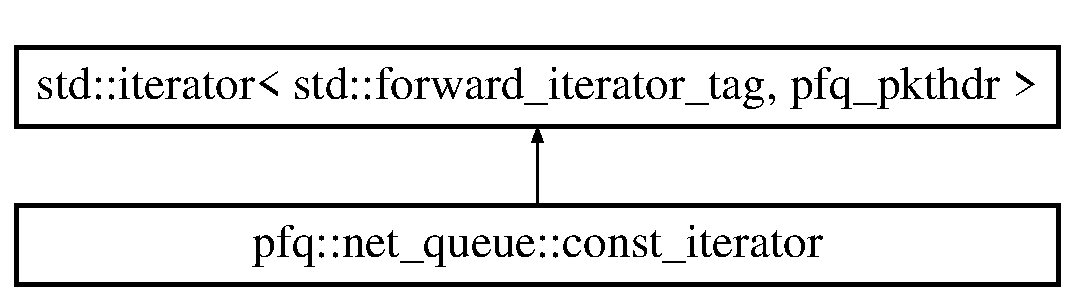
\includegraphics[height=2.000000cm]{structpfq_1_1net__queue_1_1const__iterator}
\end{center}
\end{figure}
\subsection*{Public Member Functions}
\begin{DoxyCompactItemize}
\item 
\hyperlink{structpfq_1_1net__queue_1_1const__iterator_adef1573899cd3f86946660ac3e1d4b0b}{const\+\_\+iterator} (pfq\+\_\+pkthdr $\ast$h, size\+\_\+t \hyperlink{classpfq_1_1net__queue_a29b652b2c4e672bdfe65709483ad4319}{slot\+\_\+size}, size\+\_\+t \hyperlink{classpfq_1_1net__queue_a6f328cf50f038056f2b761bfaeca4c91}{index})
\item 
\hyperlink{structpfq_1_1net__queue_1_1const__iterator_a4ebcb8be6a56b2a132b5ecb6450a253f}{const\+\_\+iterator} (const \hyperlink{structpfq_1_1net__queue_1_1const__iterator}{const\+\_\+iterator} \&other)
\item 
\hyperlink{structpfq_1_1net__queue_1_1const__iterator_ad9eae4275472c07254d3d561a50cf5f0}{const\+\_\+iterator} (const \hyperlink{structpfq_1_1net__queue_1_1iterator}{net\+\_\+queue\+::iterator} \&other)
\item 
\hyperlink{structpfq_1_1net__queue_1_1const__iterator_ab5533378a3b4b5b9aa0f8b2b43f33cf5}{$\sim$const\+\_\+iterator} ()=default
\item 
\hyperlink{structpfq_1_1net__queue_1_1const__iterator}{const\+\_\+iterator} \& \hyperlink{structpfq_1_1net__queue_1_1const__iterator_a7f460bac19b566ae12820ba8e0aa476f}{operator++} ()
\item 
\hyperlink{structpfq_1_1net__queue_1_1const__iterator}{const\+\_\+iterator} \hyperlink{structpfq_1_1net__queue_1_1const__iterator_a7a38cf885fe28b63309e88c6d1d92b00}{operator++} (int)
\item 
const pfq\+\_\+pkthdr $\ast$ \hyperlink{structpfq_1_1net__queue_1_1const__iterator_aec46f19d1306193a434aeb009437664b}{operator-\/$>$} () const
\item 
const pfq\+\_\+pkthdr \& \hyperlink{structpfq_1_1net__queue_1_1const__iterator_aee86a5a178f44829ca9ea971748577b4}{operator$\ast$} () const
\item 
const void $\ast$ \hyperlink{structpfq_1_1net__queue_1_1const__iterator_a47a268a78aa534b3cf064c58e69320b3}{data} () const
\item 
bool \hyperlink{structpfq_1_1net__queue_1_1const__iterator_aa086fec495f365981c86348de5750f7b}{ready} () const
\item 
bool \hyperlink{structpfq_1_1net__queue_1_1const__iterator_a4b38c35b765584ef7235abf6ff09398c}{operator==} (const \hyperlink{structpfq_1_1net__queue_1_1const__iterator}{const\+\_\+iterator} \&other) const
\item 
bool \hyperlink{structpfq_1_1net__queue_1_1const__iterator_acfde8b0d1f4a9183cc1b1886ae74c1f9}{operator!=} (const \hyperlink{structpfq_1_1net__queue_1_1const__iterator}{const\+\_\+iterator} \&other) const
\end{DoxyCompactItemize}


\subsection{Detailed Description}
Constant forward iterator over packets. 

\subsection{Constructor \& Destructor Documentation}
\mbox{\Hypertarget{structpfq_1_1net__queue_1_1const__iterator_adef1573899cd3f86946660ac3e1d4b0b}\label{structpfq_1_1net__queue_1_1const__iterator_adef1573899cd3f86946660ac3e1d4b0b}} 
\index{pfq\+::net\+\_\+queue\+::const\+\_\+iterator@{pfq\+::net\+\_\+queue\+::const\+\_\+iterator}!const\+\_\+iterator@{const\+\_\+iterator}}
\index{const\+\_\+iterator@{const\+\_\+iterator}!pfq\+::net\+\_\+queue\+::const\+\_\+iterator@{pfq\+::net\+\_\+queue\+::const\+\_\+iterator}}
\subsubsection{\texorpdfstring{const\+\_\+iterator()}{const\_iterator()}\hspace{0.1cm}{\footnotesize\ttfamily [1/3]}}
{\footnotesize\ttfamily pfq\+::net\+\_\+queue\+::const\+\_\+iterator\+::const\+\_\+iterator (\begin{DoxyParamCaption}\item[{pfq\+\_\+pkthdr $\ast$}]{h,  }\item[{size\+\_\+t}]{slot\+\_\+size,  }\item[{size\+\_\+t}]{index }\end{DoxyParamCaption})\hspace{0.3cm}{\ttfamily [inline]}}

\mbox{\Hypertarget{structpfq_1_1net__queue_1_1const__iterator_a4ebcb8be6a56b2a132b5ecb6450a253f}\label{structpfq_1_1net__queue_1_1const__iterator_a4ebcb8be6a56b2a132b5ecb6450a253f}} 
\index{pfq\+::net\+\_\+queue\+::const\+\_\+iterator@{pfq\+::net\+\_\+queue\+::const\+\_\+iterator}!const\+\_\+iterator@{const\+\_\+iterator}}
\index{const\+\_\+iterator@{const\+\_\+iterator}!pfq\+::net\+\_\+queue\+::const\+\_\+iterator@{pfq\+::net\+\_\+queue\+::const\+\_\+iterator}}
\subsubsection{\texorpdfstring{const\+\_\+iterator()}{const\_iterator()}\hspace{0.1cm}{\footnotesize\ttfamily [2/3]}}
{\footnotesize\ttfamily pfq\+::net\+\_\+queue\+::const\+\_\+iterator\+::const\+\_\+iterator (\begin{DoxyParamCaption}\item[{const \hyperlink{structpfq_1_1net__queue_1_1const__iterator}{const\+\_\+iterator} \&}]{other }\end{DoxyParamCaption})\hspace{0.3cm}{\ttfamily [inline]}}

\mbox{\Hypertarget{structpfq_1_1net__queue_1_1const__iterator_ad9eae4275472c07254d3d561a50cf5f0}\label{structpfq_1_1net__queue_1_1const__iterator_ad9eae4275472c07254d3d561a50cf5f0}} 
\index{pfq\+::net\+\_\+queue\+::const\+\_\+iterator@{pfq\+::net\+\_\+queue\+::const\+\_\+iterator}!const\+\_\+iterator@{const\+\_\+iterator}}
\index{const\+\_\+iterator@{const\+\_\+iterator}!pfq\+::net\+\_\+queue\+::const\+\_\+iterator@{pfq\+::net\+\_\+queue\+::const\+\_\+iterator}}
\subsubsection{\texorpdfstring{const\+\_\+iterator()}{const\_iterator()}\hspace{0.1cm}{\footnotesize\ttfamily [3/3]}}
{\footnotesize\ttfamily pfq\+::net\+\_\+queue\+::const\+\_\+iterator\+::const\+\_\+iterator (\begin{DoxyParamCaption}\item[{const \hyperlink{structpfq_1_1net__queue_1_1iterator}{net\+\_\+queue\+::iterator} \&}]{other }\end{DoxyParamCaption})\hspace{0.3cm}{\ttfamily [inline]}}

\mbox{\Hypertarget{structpfq_1_1net__queue_1_1const__iterator_ab5533378a3b4b5b9aa0f8b2b43f33cf5}\label{structpfq_1_1net__queue_1_1const__iterator_ab5533378a3b4b5b9aa0f8b2b43f33cf5}} 
\index{pfq\+::net\+\_\+queue\+::const\+\_\+iterator@{pfq\+::net\+\_\+queue\+::const\+\_\+iterator}!````~const\+\_\+iterator@{$\sim$const\+\_\+iterator}}
\index{````~const\+\_\+iterator@{$\sim$const\+\_\+iterator}!pfq\+::net\+\_\+queue\+::const\+\_\+iterator@{pfq\+::net\+\_\+queue\+::const\+\_\+iterator}}
\subsubsection{\texorpdfstring{$\sim$const\+\_\+iterator()}{~const\_iterator()}}
{\footnotesize\ttfamily pfq\+::net\+\_\+queue\+::const\+\_\+iterator\+::$\sim$const\+\_\+iterator (\begin{DoxyParamCaption}{ }\end{DoxyParamCaption})\hspace{0.3cm}{\ttfamily [default]}}



\subsection{Member Function Documentation}
\mbox{\Hypertarget{structpfq_1_1net__queue_1_1const__iterator_a47a268a78aa534b3cf064c58e69320b3}\label{structpfq_1_1net__queue_1_1const__iterator_a47a268a78aa534b3cf064c58e69320b3}} 
\index{pfq\+::net\+\_\+queue\+::const\+\_\+iterator@{pfq\+::net\+\_\+queue\+::const\+\_\+iterator}!data@{data}}
\index{data@{data}!pfq\+::net\+\_\+queue\+::const\+\_\+iterator@{pfq\+::net\+\_\+queue\+::const\+\_\+iterator}}
\subsubsection{\texorpdfstring{data()}{data()}}
{\footnotesize\ttfamily const void$\ast$ pfq\+::net\+\_\+queue\+::const\+\_\+iterator\+::data (\begin{DoxyParamCaption}{ }\end{DoxyParamCaption}) const\hspace{0.3cm}{\ttfamily [inline]}}

\mbox{\Hypertarget{structpfq_1_1net__queue_1_1const__iterator_acfde8b0d1f4a9183cc1b1886ae74c1f9}\label{structpfq_1_1net__queue_1_1const__iterator_acfde8b0d1f4a9183cc1b1886ae74c1f9}} 
\index{pfq\+::net\+\_\+queue\+::const\+\_\+iterator@{pfq\+::net\+\_\+queue\+::const\+\_\+iterator}!operator"!=@{operator"!=}}
\index{operator"!=@{operator"!=}!pfq\+::net\+\_\+queue\+::const\+\_\+iterator@{pfq\+::net\+\_\+queue\+::const\+\_\+iterator}}
\subsubsection{\texorpdfstring{operator"!=()}{operator!=()}}
{\footnotesize\ttfamily bool pfq\+::net\+\_\+queue\+::const\+\_\+iterator\+::operator!= (\begin{DoxyParamCaption}\item[{const \hyperlink{structpfq_1_1net__queue_1_1const__iterator}{const\+\_\+iterator} \&}]{other }\end{DoxyParamCaption}) const\hspace{0.3cm}{\ttfamily [inline]}}

\mbox{\Hypertarget{structpfq_1_1net__queue_1_1const__iterator_aee86a5a178f44829ca9ea971748577b4}\label{structpfq_1_1net__queue_1_1const__iterator_aee86a5a178f44829ca9ea971748577b4}} 
\index{pfq\+::net\+\_\+queue\+::const\+\_\+iterator@{pfq\+::net\+\_\+queue\+::const\+\_\+iterator}!operator$\ast$@{operator$\ast$}}
\index{operator$\ast$@{operator$\ast$}!pfq\+::net\+\_\+queue\+::const\+\_\+iterator@{pfq\+::net\+\_\+queue\+::const\+\_\+iterator}}
\subsubsection{\texorpdfstring{operator$\ast$()}{operator*()}}
{\footnotesize\ttfamily const pfq\+\_\+pkthdr\& pfq\+::net\+\_\+queue\+::const\+\_\+iterator\+::operator$\ast$ (\begin{DoxyParamCaption}{ }\end{DoxyParamCaption}) const\hspace{0.3cm}{\ttfamily [inline]}}

\mbox{\Hypertarget{structpfq_1_1net__queue_1_1const__iterator_a7f460bac19b566ae12820ba8e0aa476f}\label{structpfq_1_1net__queue_1_1const__iterator_a7f460bac19b566ae12820ba8e0aa476f}} 
\index{pfq\+::net\+\_\+queue\+::const\+\_\+iterator@{pfq\+::net\+\_\+queue\+::const\+\_\+iterator}!operator++@{operator++}}
\index{operator++@{operator++}!pfq\+::net\+\_\+queue\+::const\+\_\+iterator@{pfq\+::net\+\_\+queue\+::const\+\_\+iterator}}
\subsubsection{\texorpdfstring{operator++()}{operator++()}\hspace{0.1cm}{\footnotesize\ttfamily [1/2]}}
{\footnotesize\ttfamily \hyperlink{structpfq_1_1net__queue_1_1const__iterator}{const\+\_\+iterator}\& pfq\+::net\+\_\+queue\+::const\+\_\+iterator\+::operator++ (\begin{DoxyParamCaption}{ }\end{DoxyParamCaption})\hspace{0.3cm}{\ttfamily [inline]}}

\mbox{\Hypertarget{structpfq_1_1net__queue_1_1const__iterator_a7a38cf885fe28b63309e88c6d1d92b00}\label{structpfq_1_1net__queue_1_1const__iterator_a7a38cf885fe28b63309e88c6d1d92b00}} 
\index{pfq\+::net\+\_\+queue\+::const\+\_\+iterator@{pfq\+::net\+\_\+queue\+::const\+\_\+iterator}!operator++@{operator++}}
\index{operator++@{operator++}!pfq\+::net\+\_\+queue\+::const\+\_\+iterator@{pfq\+::net\+\_\+queue\+::const\+\_\+iterator}}
\subsubsection{\texorpdfstring{operator++()}{operator++()}\hspace{0.1cm}{\footnotesize\ttfamily [2/2]}}
{\footnotesize\ttfamily \hyperlink{structpfq_1_1net__queue_1_1const__iterator}{const\+\_\+iterator} pfq\+::net\+\_\+queue\+::const\+\_\+iterator\+::operator++ (\begin{DoxyParamCaption}\item[{int}]{ }\end{DoxyParamCaption})\hspace{0.3cm}{\ttfamily [inline]}}

\mbox{\Hypertarget{structpfq_1_1net__queue_1_1const__iterator_aec46f19d1306193a434aeb009437664b}\label{structpfq_1_1net__queue_1_1const__iterator_aec46f19d1306193a434aeb009437664b}} 
\index{pfq\+::net\+\_\+queue\+::const\+\_\+iterator@{pfq\+::net\+\_\+queue\+::const\+\_\+iterator}!operator-\/$>$@{operator-\/$>$}}
\index{operator-\/$>$@{operator-\/$>$}!pfq\+::net\+\_\+queue\+::const\+\_\+iterator@{pfq\+::net\+\_\+queue\+::const\+\_\+iterator}}
\subsubsection{\texorpdfstring{operator-\/$>$()}{operator->()}}
{\footnotesize\ttfamily const pfq\+\_\+pkthdr$\ast$ pfq\+::net\+\_\+queue\+::const\+\_\+iterator\+::operator-\/$>$ (\begin{DoxyParamCaption}{ }\end{DoxyParamCaption}) const\hspace{0.3cm}{\ttfamily [inline]}}

\mbox{\Hypertarget{structpfq_1_1net__queue_1_1const__iterator_a4b38c35b765584ef7235abf6ff09398c}\label{structpfq_1_1net__queue_1_1const__iterator_a4b38c35b765584ef7235abf6ff09398c}} 
\index{pfq\+::net\+\_\+queue\+::const\+\_\+iterator@{pfq\+::net\+\_\+queue\+::const\+\_\+iterator}!operator==@{operator==}}
\index{operator==@{operator==}!pfq\+::net\+\_\+queue\+::const\+\_\+iterator@{pfq\+::net\+\_\+queue\+::const\+\_\+iterator}}
\subsubsection{\texorpdfstring{operator==()}{operator==()}}
{\footnotesize\ttfamily bool pfq\+::net\+\_\+queue\+::const\+\_\+iterator\+::operator== (\begin{DoxyParamCaption}\item[{const \hyperlink{structpfq_1_1net__queue_1_1const__iterator}{const\+\_\+iterator} \&}]{other }\end{DoxyParamCaption}) const\hspace{0.3cm}{\ttfamily [inline]}}

\mbox{\Hypertarget{structpfq_1_1net__queue_1_1const__iterator_aa086fec495f365981c86348de5750f7b}\label{structpfq_1_1net__queue_1_1const__iterator_aa086fec495f365981c86348de5750f7b}} 
\index{pfq\+::net\+\_\+queue\+::const\+\_\+iterator@{pfq\+::net\+\_\+queue\+::const\+\_\+iterator}!ready@{ready}}
\index{ready@{ready}!pfq\+::net\+\_\+queue\+::const\+\_\+iterator@{pfq\+::net\+\_\+queue\+::const\+\_\+iterator}}
\subsubsection{\texorpdfstring{ready()}{ready()}}
{\footnotesize\ttfamily bool pfq\+::net\+\_\+queue\+::const\+\_\+iterator\+::ready (\begin{DoxyParamCaption}{ }\end{DoxyParamCaption}) const\hspace{0.3cm}{\ttfamily [inline]}}



The documentation for this struct was generated from the following file\+:\begin{DoxyCompactItemize}
\item 
C++/pfq/\hyperlink{queue_8hpp}{queue.\+hpp}\end{DoxyCompactItemize}

\hypertarget{structpfq_1_1net__queue_1_1iterator}{\section{pfq\+:\+:net\+\_\+queue\+:\+:iterator Struct Reference}
\label{structpfq_1_1net__queue_1_1iterator}\index{pfq\+::net\+\_\+queue\+::iterator@{pfq\+::net\+\_\+queue\+::iterator}}
}


Forward iterator over packets.  




{\ttfamily \#include $<$queue.\+hpp$>$}

Inheritance diagram for pfq\+:\+:net\+\_\+queue\+:\+:iterator\+:\begin{figure}[H]
\begin{center}
\leavevmode
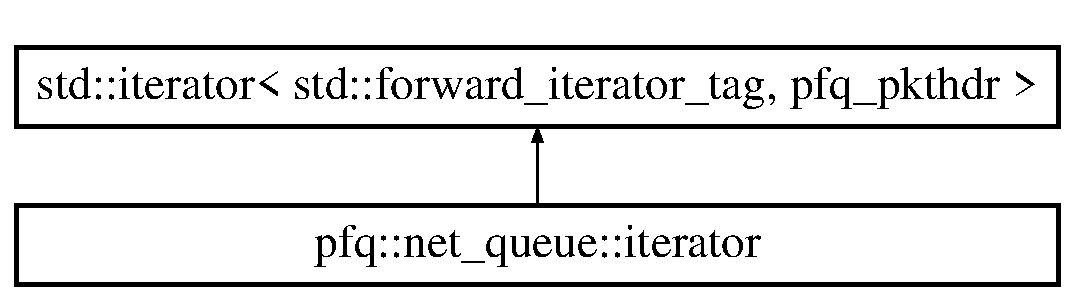
\includegraphics[height=2.000000cm]{structpfq_1_1net__queue_1_1iterator}
\end{center}
\end{figure}
\subsection*{Public Member Functions}
\begin{DoxyCompactItemize}
\item 
\hyperlink{structpfq_1_1net__queue_1_1iterator_a32b5b8db4f59df4c074e0aafe98c79a5}{iterator} (pfq\+\_\+pkthdr $\ast$h, size\+\_\+t \hyperlink{classpfq_1_1net__queue_a9f745871293123f417a492aa861c13cc}{slot\+\_\+size}, size\+\_\+t \hyperlink{classpfq_1_1net__queue_ab33bdebd885e677a3e079c0193624e52}{index})
\item 
\hyperlink{structpfq_1_1net__queue_1_1iterator_a796f1d97807c57026713f2664bf992bc}{$\sim$iterator} ()=default
\item 
\hyperlink{structpfq_1_1net__queue_1_1iterator_a49a7278fa0b900830b46675c1365d370}{iterator} (const \hyperlink{structpfq_1_1net__queue_1_1iterator}{iterator} \&other)
\item 
\hyperlink{structpfq_1_1net__queue_1_1iterator}{iterator} \& \hyperlink{structpfq_1_1net__queue_1_1iterator_a4e7bf9ea9183af5efd3ade9a50e3350c}{operator++} ()
\item 
\hyperlink{structpfq_1_1net__queue_1_1iterator}{iterator} \hyperlink{structpfq_1_1net__queue_1_1iterator_ad108401f7fd2b6df0fa885ab651cc2fa}{operator++} (int)
\item 
pfq\+\_\+pkthdr $\ast$ \hyperlink{structpfq_1_1net__queue_1_1iterator_ae8bef3a6b332d22fff606e4aeaa6a1d0}{operator-\/$>$} () const 
\item 
pfq\+\_\+pkthdr \& \hyperlink{structpfq_1_1net__queue_1_1iterator_a8ba14cea90784881ea3b31fe0ef33c3c}{operator$\ast$} () const 
\item 
void $\ast$ \hyperlink{structpfq_1_1net__queue_1_1iterator_aa7f321b403fbd77d168478475ae5bd3c}{data} () const 
\item 
bool \hyperlink{structpfq_1_1net__queue_1_1iterator_a878ca2b92a0e25589a8b986c18ff7885}{ready} () const 
\item 
bool \hyperlink{structpfq_1_1net__queue_1_1iterator_a16c662d3c3dc43b6354b78a308376826}{operator==} (const \hyperlink{structpfq_1_1net__queue_1_1iterator}{iterator} \&other) const 
\item 
bool \hyperlink{structpfq_1_1net__queue_1_1iterator_a789cabd61a87acc677d2f565d0c043f4}{operator!=} (const \hyperlink{structpfq_1_1net__queue_1_1iterator}{iterator} \&other) const 
\end{DoxyCompactItemize}
\subsection*{Friends}
\begin{DoxyCompactItemize}
\item 
struct \hyperlink{structpfq_1_1net__queue_1_1iterator_a0fa1c59b5fb1d453f45032bc7a6ea3b0}{net\+\_\+queue\+::const\+\_\+iterator}
\end{DoxyCompactItemize}


\subsection{Detailed Description}
Forward iterator over packets. 

\subsection{Constructor \& Destructor Documentation}
\hypertarget{structpfq_1_1net__queue_1_1iterator_a32b5b8db4f59df4c074e0aafe98c79a5}{\index{pfq\+::net\+\_\+queue\+::iterator@{pfq\+::net\+\_\+queue\+::iterator}!iterator@{iterator}}
\index{iterator@{iterator}!pfq\+::net\+\_\+queue\+::iterator@{pfq\+::net\+\_\+queue\+::iterator}}
\subsubsection[{iterator}]{\setlength{\rightskip}{0pt plus 5cm}pfq\+::net\+\_\+queue\+::iterator\+::iterator (
\begin{DoxyParamCaption}
\item[{pfq\+\_\+pkthdr $\ast$}]{h, }
\item[{size\+\_\+t}]{slot\+\_\+size, }
\item[{size\+\_\+t}]{index}
\end{DoxyParamCaption}
)\hspace{0.3cm}{\ttfamily [inline]}}}\label{structpfq_1_1net__queue_1_1iterator_a32b5b8db4f59df4c074e0aafe98c79a5}
\hypertarget{structpfq_1_1net__queue_1_1iterator_a796f1d97807c57026713f2664bf992bc}{\index{pfq\+::net\+\_\+queue\+::iterator@{pfq\+::net\+\_\+queue\+::iterator}!````~iterator@{$\sim$iterator}}
\index{````~iterator@{$\sim$iterator}!pfq\+::net\+\_\+queue\+::iterator@{pfq\+::net\+\_\+queue\+::iterator}}
\subsubsection[{$\sim$iterator}]{\setlength{\rightskip}{0pt plus 5cm}pfq\+::net\+\_\+queue\+::iterator\+::$\sim$iterator (
\begin{DoxyParamCaption}
{}
\end{DoxyParamCaption}
)\hspace{0.3cm}{\ttfamily [default]}}}\label{structpfq_1_1net__queue_1_1iterator_a796f1d97807c57026713f2664bf992bc}
\hypertarget{structpfq_1_1net__queue_1_1iterator_a49a7278fa0b900830b46675c1365d370}{\index{pfq\+::net\+\_\+queue\+::iterator@{pfq\+::net\+\_\+queue\+::iterator}!iterator@{iterator}}
\index{iterator@{iterator}!pfq\+::net\+\_\+queue\+::iterator@{pfq\+::net\+\_\+queue\+::iterator}}
\subsubsection[{iterator}]{\setlength{\rightskip}{0pt plus 5cm}pfq\+::net\+\_\+queue\+::iterator\+::iterator (
\begin{DoxyParamCaption}
\item[{const {\bf iterator} \&}]{other}
\end{DoxyParamCaption}
)\hspace{0.3cm}{\ttfamily [inline]}}}\label{structpfq_1_1net__queue_1_1iterator_a49a7278fa0b900830b46675c1365d370}


\subsection{Member Function Documentation}
\hypertarget{structpfq_1_1net__queue_1_1iterator_aa7f321b403fbd77d168478475ae5bd3c}{\index{pfq\+::net\+\_\+queue\+::iterator@{pfq\+::net\+\_\+queue\+::iterator}!data@{data}}
\index{data@{data}!pfq\+::net\+\_\+queue\+::iterator@{pfq\+::net\+\_\+queue\+::iterator}}
\subsubsection[{data}]{\setlength{\rightskip}{0pt plus 5cm}void$\ast$ pfq\+::net\+\_\+queue\+::iterator\+::data (
\begin{DoxyParamCaption}
{}
\end{DoxyParamCaption}
) const\hspace{0.3cm}{\ttfamily [inline]}}}\label{structpfq_1_1net__queue_1_1iterator_aa7f321b403fbd77d168478475ae5bd3c}
\hypertarget{structpfq_1_1net__queue_1_1iterator_a789cabd61a87acc677d2f565d0c043f4}{\index{pfq\+::net\+\_\+queue\+::iterator@{pfq\+::net\+\_\+queue\+::iterator}!operator"!=@{operator"!=}}
\index{operator"!=@{operator"!=}!pfq\+::net\+\_\+queue\+::iterator@{pfq\+::net\+\_\+queue\+::iterator}}
\subsubsection[{operator"!=}]{\setlength{\rightskip}{0pt plus 5cm}bool pfq\+::net\+\_\+queue\+::iterator\+::operator!= (
\begin{DoxyParamCaption}
\item[{const {\bf iterator} \&}]{other}
\end{DoxyParamCaption}
) const\hspace{0.3cm}{\ttfamily [inline]}}}\label{structpfq_1_1net__queue_1_1iterator_a789cabd61a87acc677d2f565d0c043f4}
\hypertarget{structpfq_1_1net__queue_1_1iterator_a8ba14cea90784881ea3b31fe0ef33c3c}{\index{pfq\+::net\+\_\+queue\+::iterator@{pfq\+::net\+\_\+queue\+::iterator}!operator$\ast$@{operator$\ast$}}
\index{operator$\ast$@{operator$\ast$}!pfq\+::net\+\_\+queue\+::iterator@{pfq\+::net\+\_\+queue\+::iterator}}
\subsubsection[{operator$\ast$}]{\setlength{\rightskip}{0pt plus 5cm}pfq\+\_\+pkthdr\& pfq\+::net\+\_\+queue\+::iterator\+::operator$\ast$ (
\begin{DoxyParamCaption}
{}
\end{DoxyParamCaption}
) const\hspace{0.3cm}{\ttfamily [inline]}}}\label{structpfq_1_1net__queue_1_1iterator_a8ba14cea90784881ea3b31fe0ef33c3c}
\hypertarget{structpfq_1_1net__queue_1_1iterator_a4e7bf9ea9183af5efd3ade9a50e3350c}{\index{pfq\+::net\+\_\+queue\+::iterator@{pfq\+::net\+\_\+queue\+::iterator}!operator++@{operator++}}
\index{operator++@{operator++}!pfq\+::net\+\_\+queue\+::iterator@{pfq\+::net\+\_\+queue\+::iterator}}
\subsubsection[{operator++}]{\setlength{\rightskip}{0pt plus 5cm}{\bf iterator}\& pfq\+::net\+\_\+queue\+::iterator\+::operator++ (
\begin{DoxyParamCaption}
{}
\end{DoxyParamCaption}
)\hspace{0.3cm}{\ttfamily [inline]}}}\label{structpfq_1_1net__queue_1_1iterator_a4e7bf9ea9183af5efd3ade9a50e3350c}
\hypertarget{structpfq_1_1net__queue_1_1iterator_ad108401f7fd2b6df0fa885ab651cc2fa}{\index{pfq\+::net\+\_\+queue\+::iterator@{pfq\+::net\+\_\+queue\+::iterator}!operator++@{operator++}}
\index{operator++@{operator++}!pfq\+::net\+\_\+queue\+::iterator@{pfq\+::net\+\_\+queue\+::iterator}}
\subsubsection[{operator++}]{\setlength{\rightskip}{0pt plus 5cm}{\bf iterator} pfq\+::net\+\_\+queue\+::iterator\+::operator++ (
\begin{DoxyParamCaption}
\item[{int}]{}
\end{DoxyParamCaption}
)\hspace{0.3cm}{\ttfamily [inline]}}}\label{structpfq_1_1net__queue_1_1iterator_ad108401f7fd2b6df0fa885ab651cc2fa}
\hypertarget{structpfq_1_1net__queue_1_1iterator_ae8bef3a6b332d22fff606e4aeaa6a1d0}{\index{pfq\+::net\+\_\+queue\+::iterator@{pfq\+::net\+\_\+queue\+::iterator}!operator-\/$>$@{operator-\/$>$}}
\index{operator-\/$>$@{operator-\/$>$}!pfq\+::net\+\_\+queue\+::iterator@{pfq\+::net\+\_\+queue\+::iterator}}
\subsubsection[{operator-\/$>$}]{\setlength{\rightskip}{0pt plus 5cm}pfq\+\_\+pkthdr$\ast$ pfq\+::net\+\_\+queue\+::iterator\+::operator-\/$>$ (
\begin{DoxyParamCaption}
{}
\end{DoxyParamCaption}
) const\hspace{0.3cm}{\ttfamily [inline]}}}\label{structpfq_1_1net__queue_1_1iterator_ae8bef3a6b332d22fff606e4aeaa6a1d0}
\hypertarget{structpfq_1_1net__queue_1_1iterator_a16c662d3c3dc43b6354b78a308376826}{\index{pfq\+::net\+\_\+queue\+::iterator@{pfq\+::net\+\_\+queue\+::iterator}!operator==@{operator==}}
\index{operator==@{operator==}!pfq\+::net\+\_\+queue\+::iterator@{pfq\+::net\+\_\+queue\+::iterator}}
\subsubsection[{operator==}]{\setlength{\rightskip}{0pt plus 5cm}bool pfq\+::net\+\_\+queue\+::iterator\+::operator== (
\begin{DoxyParamCaption}
\item[{const {\bf iterator} \&}]{other}
\end{DoxyParamCaption}
) const\hspace{0.3cm}{\ttfamily [inline]}}}\label{structpfq_1_1net__queue_1_1iterator_a16c662d3c3dc43b6354b78a308376826}
\hypertarget{structpfq_1_1net__queue_1_1iterator_a878ca2b92a0e25589a8b986c18ff7885}{\index{pfq\+::net\+\_\+queue\+::iterator@{pfq\+::net\+\_\+queue\+::iterator}!ready@{ready}}
\index{ready@{ready}!pfq\+::net\+\_\+queue\+::iterator@{pfq\+::net\+\_\+queue\+::iterator}}
\subsubsection[{ready}]{\setlength{\rightskip}{0pt plus 5cm}bool pfq\+::net\+\_\+queue\+::iterator\+::ready (
\begin{DoxyParamCaption}
{}
\end{DoxyParamCaption}
) const\hspace{0.3cm}{\ttfamily [inline]}}}\label{structpfq_1_1net__queue_1_1iterator_a878ca2b92a0e25589a8b986c18ff7885}


\subsection{Friends And Related Function Documentation}
\hypertarget{structpfq_1_1net__queue_1_1iterator_a0fa1c59b5fb1d453f45032bc7a6ea3b0}{\index{pfq\+::net\+\_\+queue\+::iterator@{pfq\+::net\+\_\+queue\+::iterator}!net\+\_\+queue\+::const\+\_\+iterator@{net\+\_\+queue\+::const\+\_\+iterator}}
\index{net\+\_\+queue\+::const\+\_\+iterator@{net\+\_\+queue\+::const\+\_\+iterator}!pfq\+::net\+\_\+queue\+::iterator@{pfq\+::net\+\_\+queue\+::iterator}}
\subsubsection[{net\+\_\+queue\+::const\+\_\+iterator}]{\setlength{\rightskip}{0pt plus 5cm}friend struct {\bf net\+\_\+queue\+::const\+\_\+iterator}\hspace{0.3cm}{\ttfamily [friend]}}}\label{structpfq_1_1net__queue_1_1iterator_a0fa1c59b5fb1d453f45032bc7a6ea3b0}


The documentation for this struct was generated from the following file\+:\begin{DoxyCompactItemize}
\item 
C++/pfq/\hyperlink{queue_8hpp}{queue.\+hpp}\end{DoxyCompactItemize}

\hypertarget{classpfq_1_1net__queue}{\section{pfq\+:\+:net\+\_\+queue Class Reference}
\label{classpfq_1_1net__queue}\index{pfq\+::net\+\_\+queue@{pfq\+::net\+\_\+queue}}
}


This class represent a queue of packets.  




{\ttfamily \#include $<$queue.\+hpp$>$}

\subsection*{Classes}
\begin{DoxyCompactItemize}
\item 
struct \hyperlink{structpfq_1_1net__queue_1_1const__iterator}{const\+\_\+iterator}
\begin{DoxyCompactList}\small\item\em Constant forward iterator over packets. \end{DoxyCompactList}\item 
struct \hyperlink{structpfq_1_1net__queue_1_1iterator}{iterator}
\begin{DoxyCompactList}\small\item\em Forward iterator over packets. \end{DoxyCompactList}\end{DoxyCompactItemize}
\subsection*{Public Member Functions}
\begin{DoxyCompactItemize}
\item 
\hyperlink{classpfq_1_1net__queue_a1306ad9a1587c85ac3bafc552667a578}{net\+\_\+queue} ()
\begin{DoxyCompactList}\small\item\em Default Constructor. \end{DoxyCompactList}\item 
\hyperlink{classpfq_1_1net__queue_a3e98f8f2ae6dfd4a0e7d28734601d307}{net\+\_\+queue} (void $\ast$addr, size\+\_\+t \hyperlink{classpfq_1_1net__queue_a9f745871293123f417a492aa861c13cc}{slot\+\_\+size}, size\+\_\+t queue\+\_\+len, size\+\_\+t \hyperlink{classpfq_1_1net__queue_ab33bdebd885e677a3e079c0193624e52}{index})
\begin{DoxyCompactList}\small\item\em Constructor. \end{DoxyCompactList}\item 
\hyperlink{classpfq_1_1net__queue_a71df078739d1e6a0817ac8bde9fa6f7a}{net\+\_\+queue} (\hyperlink{classpfq_1_1net__queue}{net\+\_\+queue} const \&)=default
\begin{DoxyCompactList}\small\item\em Defaulted copy constructor. \end{DoxyCompactList}\item 
\hyperlink{classpfq_1_1net__queue_a87fd3585cac30773e7f5ff6951e74957}{$\sim$net\+\_\+queue} ()=default
\begin{DoxyCompactList}\small\item\em Defaulted destructor. \end{DoxyCompactList}\item 
size\+\_\+t \hyperlink{classpfq_1_1net__queue_a3c7e453d47e5493300312c0359e1497b}{size} () const 
\begin{DoxyCompactList}\small\item\em Return the number of packets stored in this queue. \end{DoxyCompactList}\item 
bool \hyperlink{classpfq_1_1net__queue_a3e59c334176f5910f4a204965d4442b9}{empty} () const 
\begin{DoxyCompactList}\small\item\em Check whether the queue is empty. \end{DoxyCompactList}\item 
size\+\_\+t \hyperlink{classpfq_1_1net__queue_ab33bdebd885e677a3e079c0193624e52}{index} () const 
\begin{DoxyCompactList}\small\item\em Return the index position. \end{DoxyCompactList}\item 
size\+\_\+t \hyperlink{classpfq_1_1net__queue_a9f745871293123f417a492aa861c13cc}{slot\+\_\+size} () const 
\begin{DoxyCompactList}\small\item\em Return the size of the queue slot, in bytes. \end{DoxyCompactList}\item 
const void $\ast$ \hyperlink{classpfq_1_1net__queue_a28a03d4dbdf57d4bc70266a174d34514}{data} () const 
\begin{DoxyCompactList}\small\item\em Return the pointer to the packet. \end{DoxyCompactList}\item 
\hyperlink{structpfq_1_1net__queue_1_1iterator}{iterator} \hyperlink{classpfq_1_1net__queue_a36d91779a4ac2a6e3f7e63ff8594ada7}{begin} ()
\begin{DoxyCompactList}\small\item\em Return an iterator to the first slot of a non-\/empty queue. \end{DoxyCompactList}\item 
\hyperlink{structpfq_1_1net__queue_1_1const__iterator}{const\+\_\+iterator} \hyperlink{classpfq_1_1net__queue_a1355ab3d8cd90fa8dafb6b5d44aef22c}{begin} () const 
\begin{DoxyCompactList}\small\item\em Return a constant iterator to the first slot of a non-\/empty queue. \end{DoxyCompactList}\item 
\hyperlink{structpfq_1_1net__queue_1_1iterator}{iterator} \hyperlink{classpfq_1_1net__queue_acef930aef921f06803621af79f993b25}{end} ()
\begin{DoxyCompactList}\small\item\em Return an iterator past to the end of the queue. \end{DoxyCompactList}\item 
\hyperlink{structpfq_1_1net__queue_1_1const__iterator}{const\+\_\+iterator} \hyperlink{classpfq_1_1net__queue_aa756544d9d17ce6d0ede19328f7dda44}{end} () const 
\begin{DoxyCompactList}\small\item\em Return a constant iterator past to the end of the queue. \end{DoxyCompactList}\item 
\hyperlink{structpfq_1_1net__queue_1_1const__iterator}{const\+\_\+iterator} \hyperlink{classpfq_1_1net__queue_a301029d6e206c848a48b7bee5e214693}{cbegin} () const 
\begin{DoxyCompactList}\small\item\em Return a constant iterator to the first slot of an non-\/empty queue. \end{DoxyCompactList}\item 
\hyperlink{structpfq_1_1net__queue_1_1const__iterator}{const\+\_\+iterator} \hyperlink{classpfq_1_1net__queue_acf4518bbd21fee1d4ab3fb36ef8be323}{cend} () const 
\begin{DoxyCompactList}\small\item\em Return a constant iterator past to the end of the queue. \end{DoxyCompactList}\end{DoxyCompactItemize}


\subsection{Detailed Description}
This class represent a queue of packets. 

The memory where packets are stored is not owned by this class. 

\subsection{Constructor \& Destructor Documentation}
\hypertarget{classpfq_1_1net__queue_a1306ad9a1587c85ac3bafc552667a578}{\index{pfq\+::net\+\_\+queue@{pfq\+::net\+\_\+queue}!net\+\_\+queue@{net\+\_\+queue}}
\index{net\+\_\+queue@{net\+\_\+queue}!pfq\+::net\+\_\+queue@{pfq\+::net\+\_\+queue}}
\subsubsection[{net\+\_\+queue}]{\setlength{\rightskip}{0pt plus 5cm}pfq\+::net\+\_\+queue\+::net\+\_\+queue (
\begin{DoxyParamCaption}
{}
\end{DoxyParamCaption}
)\hspace{0.3cm}{\ttfamily [inline]}}}\label{classpfq_1_1net__queue_a1306ad9a1587c85ac3bafc552667a578}


Default Constructor. 

\hypertarget{classpfq_1_1net__queue_a3e98f8f2ae6dfd4a0e7d28734601d307}{\index{pfq\+::net\+\_\+queue@{pfq\+::net\+\_\+queue}!net\+\_\+queue@{net\+\_\+queue}}
\index{net\+\_\+queue@{net\+\_\+queue}!pfq\+::net\+\_\+queue@{pfq\+::net\+\_\+queue}}
\subsubsection[{net\+\_\+queue}]{\setlength{\rightskip}{0pt plus 5cm}pfq\+::net\+\_\+queue\+::net\+\_\+queue (
\begin{DoxyParamCaption}
\item[{void $\ast$}]{addr, }
\item[{size\+\_\+t}]{slot\+\_\+size, }
\item[{size\+\_\+t}]{queue\+\_\+len, }
\item[{size\+\_\+t}]{index}
\end{DoxyParamCaption}
)\hspace{0.3cm}{\ttfamily [inline]}}}\label{classpfq_1_1net__queue_a3e98f8f2ae6dfd4a0e7d28734601d307}


Constructor. 

\hypertarget{classpfq_1_1net__queue_a71df078739d1e6a0817ac8bde9fa6f7a}{\index{pfq\+::net\+\_\+queue@{pfq\+::net\+\_\+queue}!net\+\_\+queue@{net\+\_\+queue}}
\index{net\+\_\+queue@{net\+\_\+queue}!pfq\+::net\+\_\+queue@{pfq\+::net\+\_\+queue}}
\subsubsection[{net\+\_\+queue}]{\setlength{\rightskip}{0pt plus 5cm}pfq\+::net\+\_\+queue\+::net\+\_\+queue (
\begin{DoxyParamCaption}
\item[{{\bf net\+\_\+queue} const \&}]{}
\end{DoxyParamCaption}
)\hspace{0.3cm}{\ttfamily [default]}}}\label{classpfq_1_1net__queue_a71df078739d1e6a0817ac8bde9fa6f7a}


Defaulted copy constructor. 

\hypertarget{classpfq_1_1net__queue_a87fd3585cac30773e7f5ff6951e74957}{\index{pfq\+::net\+\_\+queue@{pfq\+::net\+\_\+queue}!````~net\+\_\+queue@{$\sim$net\+\_\+queue}}
\index{````~net\+\_\+queue@{$\sim$net\+\_\+queue}!pfq\+::net\+\_\+queue@{pfq\+::net\+\_\+queue}}
\subsubsection[{$\sim$net\+\_\+queue}]{\setlength{\rightskip}{0pt plus 5cm}pfq\+::net\+\_\+queue\+::$\sim$net\+\_\+queue (
\begin{DoxyParamCaption}
{}
\end{DoxyParamCaption}
)\hspace{0.3cm}{\ttfamily [default]}}}\label{classpfq_1_1net__queue_a87fd3585cac30773e7f5ff6951e74957}


Defaulted destructor. 



\subsection{Member Function Documentation}
\hypertarget{classpfq_1_1net__queue_a36d91779a4ac2a6e3f7e63ff8594ada7}{\index{pfq\+::net\+\_\+queue@{pfq\+::net\+\_\+queue}!begin@{begin}}
\index{begin@{begin}!pfq\+::net\+\_\+queue@{pfq\+::net\+\_\+queue}}
\subsubsection[{begin}]{\setlength{\rightskip}{0pt plus 5cm}{\bf iterator} pfq\+::net\+\_\+queue\+::begin (
\begin{DoxyParamCaption}
{}
\end{DoxyParamCaption}
)\hspace{0.3cm}{\ttfamily [inline]}}}\label{classpfq_1_1net__queue_a36d91779a4ac2a6e3f7e63ff8594ada7}


Return an iterator to the first slot of a non-\/empty queue. 

Return \hyperlink{classpfq_1_1net__queue_acef930aef921f06803621af79f993b25}{end()} in case of empty queue. \hypertarget{classpfq_1_1net__queue_a1355ab3d8cd90fa8dafb6b5d44aef22c}{\index{pfq\+::net\+\_\+queue@{pfq\+::net\+\_\+queue}!begin@{begin}}
\index{begin@{begin}!pfq\+::net\+\_\+queue@{pfq\+::net\+\_\+queue}}
\subsubsection[{begin}]{\setlength{\rightskip}{0pt plus 5cm}{\bf const\+\_\+iterator} pfq\+::net\+\_\+queue\+::begin (
\begin{DoxyParamCaption}
{}
\end{DoxyParamCaption}
) const\hspace{0.3cm}{\ttfamily [inline]}}}\label{classpfq_1_1net__queue_a1355ab3d8cd90fa8dafb6b5d44aef22c}


Return a constant iterator to the first slot of a non-\/empty queue. 

Return \hyperlink{classpfq_1_1net__queue_acef930aef921f06803621af79f993b25}{end()} in case of empty queue. \hypertarget{classpfq_1_1net__queue_a301029d6e206c848a48b7bee5e214693}{\index{pfq\+::net\+\_\+queue@{pfq\+::net\+\_\+queue}!cbegin@{cbegin}}
\index{cbegin@{cbegin}!pfq\+::net\+\_\+queue@{pfq\+::net\+\_\+queue}}
\subsubsection[{cbegin}]{\setlength{\rightskip}{0pt plus 5cm}{\bf const\+\_\+iterator} pfq\+::net\+\_\+queue\+::cbegin (
\begin{DoxyParamCaption}
{}
\end{DoxyParamCaption}
) const\hspace{0.3cm}{\ttfamily [inline]}}}\label{classpfq_1_1net__queue_a301029d6e206c848a48b7bee5e214693}


Return a constant iterator to the first slot of an non-\/empty queue. 

Return \hyperlink{classpfq_1_1net__queue_acf4518bbd21fee1d4ab3fb36ef8be323}{cend()} in case of empty queue. \hypertarget{classpfq_1_1net__queue_acf4518bbd21fee1d4ab3fb36ef8be323}{\index{pfq\+::net\+\_\+queue@{pfq\+::net\+\_\+queue}!cend@{cend}}
\index{cend@{cend}!pfq\+::net\+\_\+queue@{pfq\+::net\+\_\+queue}}
\subsubsection[{cend}]{\setlength{\rightskip}{0pt plus 5cm}{\bf const\+\_\+iterator} pfq\+::net\+\_\+queue\+::cend (
\begin{DoxyParamCaption}
{}
\end{DoxyParamCaption}
) const\hspace{0.3cm}{\ttfamily [inline]}}}\label{classpfq_1_1net__queue_acf4518bbd21fee1d4ab3fb36ef8be323}


Return a constant iterator past to the end of the queue. 

\hypertarget{classpfq_1_1net__queue_a28a03d4dbdf57d4bc70266a174d34514}{\index{pfq\+::net\+\_\+queue@{pfq\+::net\+\_\+queue}!data@{data}}
\index{data@{data}!pfq\+::net\+\_\+queue@{pfq\+::net\+\_\+queue}}
\subsubsection[{data}]{\setlength{\rightskip}{0pt plus 5cm}const void$\ast$ pfq\+::net\+\_\+queue\+::data (
\begin{DoxyParamCaption}
{}
\end{DoxyParamCaption}
) const\hspace{0.3cm}{\ttfamily [inline]}}}\label{classpfq_1_1net__queue_a28a03d4dbdf57d4bc70266a174d34514}


Return the pointer to the packet. 

\hypertarget{classpfq_1_1net__queue_a3e59c334176f5910f4a204965d4442b9}{\index{pfq\+::net\+\_\+queue@{pfq\+::net\+\_\+queue}!empty@{empty}}
\index{empty@{empty}!pfq\+::net\+\_\+queue@{pfq\+::net\+\_\+queue}}
\subsubsection[{empty}]{\setlength{\rightskip}{0pt plus 5cm}bool pfq\+::net\+\_\+queue\+::empty (
\begin{DoxyParamCaption}
{}
\end{DoxyParamCaption}
) const\hspace{0.3cm}{\ttfamily [inline]}}}\label{classpfq_1_1net__queue_a3e59c334176f5910f4a204965d4442b9}


Check whether the queue is empty. 

\hypertarget{classpfq_1_1net__queue_acef930aef921f06803621af79f993b25}{\index{pfq\+::net\+\_\+queue@{pfq\+::net\+\_\+queue}!end@{end}}
\index{end@{end}!pfq\+::net\+\_\+queue@{pfq\+::net\+\_\+queue}}
\subsubsection[{end}]{\setlength{\rightskip}{0pt plus 5cm}{\bf iterator} pfq\+::net\+\_\+queue\+::end (
\begin{DoxyParamCaption}
{}
\end{DoxyParamCaption}
)\hspace{0.3cm}{\ttfamily [inline]}}}\label{classpfq_1_1net__queue_acef930aef921f06803621af79f993b25}


Return an iterator past to the end of the queue. 

\hypertarget{classpfq_1_1net__queue_aa756544d9d17ce6d0ede19328f7dda44}{\index{pfq\+::net\+\_\+queue@{pfq\+::net\+\_\+queue}!end@{end}}
\index{end@{end}!pfq\+::net\+\_\+queue@{pfq\+::net\+\_\+queue}}
\subsubsection[{end}]{\setlength{\rightskip}{0pt plus 5cm}{\bf const\+\_\+iterator} pfq\+::net\+\_\+queue\+::end (
\begin{DoxyParamCaption}
{}
\end{DoxyParamCaption}
) const\hspace{0.3cm}{\ttfamily [inline]}}}\label{classpfq_1_1net__queue_aa756544d9d17ce6d0ede19328f7dda44}


Return a constant iterator past to the end of the queue. 

\hypertarget{classpfq_1_1net__queue_ab33bdebd885e677a3e079c0193624e52}{\index{pfq\+::net\+\_\+queue@{pfq\+::net\+\_\+queue}!index@{index}}
\index{index@{index}!pfq\+::net\+\_\+queue@{pfq\+::net\+\_\+queue}}
\subsubsection[{index}]{\setlength{\rightskip}{0pt plus 5cm}size\+\_\+t pfq\+::net\+\_\+queue\+::index (
\begin{DoxyParamCaption}
{}
\end{DoxyParamCaption}
) const\hspace{0.3cm}{\ttfamily [inline]}}}\label{classpfq_1_1net__queue_ab33bdebd885e677a3e079c0193624e52}


Return the index position. 

\hypertarget{classpfq_1_1net__queue_a3c7e453d47e5493300312c0359e1497b}{\index{pfq\+::net\+\_\+queue@{pfq\+::net\+\_\+queue}!size@{size}}
\index{size@{size}!pfq\+::net\+\_\+queue@{pfq\+::net\+\_\+queue}}
\subsubsection[{size}]{\setlength{\rightskip}{0pt plus 5cm}size\+\_\+t pfq\+::net\+\_\+queue\+::size (
\begin{DoxyParamCaption}
{}
\end{DoxyParamCaption}
) const\hspace{0.3cm}{\ttfamily [inline]}}}\label{classpfq_1_1net__queue_a3c7e453d47e5493300312c0359e1497b}


Return the number of packets stored in this queue. 

\hypertarget{classpfq_1_1net__queue_a9f745871293123f417a492aa861c13cc}{\index{pfq\+::net\+\_\+queue@{pfq\+::net\+\_\+queue}!slot\+\_\+size@{slot\+\_\+size}}
\index{slot\+\_\+size@{slot\+\_\+size}!pfq\+::net\+\_\+queue@{pfq\+::net\+\_\+queue}}
\subsubsection[{slot\+\_\+size}]{\setlength{\rightskip}{0pt plus 5cm}size\+\_\+t pfq\+::net\+\_\+queue\+::slot\+\_\+size (
\begin{DoxyParamCaption}
{}
\end{DoxyParamCaption}
) const\hspace{0.3cm}{\ttfamily [inline]}}}\label{classpfq_1_1net__queue_a9f745871293123f417a492aa861c13cc}


Return the size of the queue slot, in bytes. 



The documentation for this class was generated from the following file\+:\begin{DoxyCompactItemize}
\item 
C++/pfq/\hyperlink{queue_8hpp}{queue.\+hpp}\end{DoxyCompactItemize}

\hypertarget{classpfq_1_1pfq__error}{\section{pfq\+:\+:pfq\+\_\+error Class Reference}
\label{classpfq_1_1pfq__error}\index{pfq\+::pfq\+\_\+error@{pfq\+::pfq\+\_\+error}}
}


Subclass of std\+::system\+\_\+error.  




{\ttfamily \#include $<$exception.\+hpp$>$}

Inheritance diagram for pfq\+:\+:pfq\+\_\+error\+:\begin{figure}[H]
\begin{center}
\leavevmode
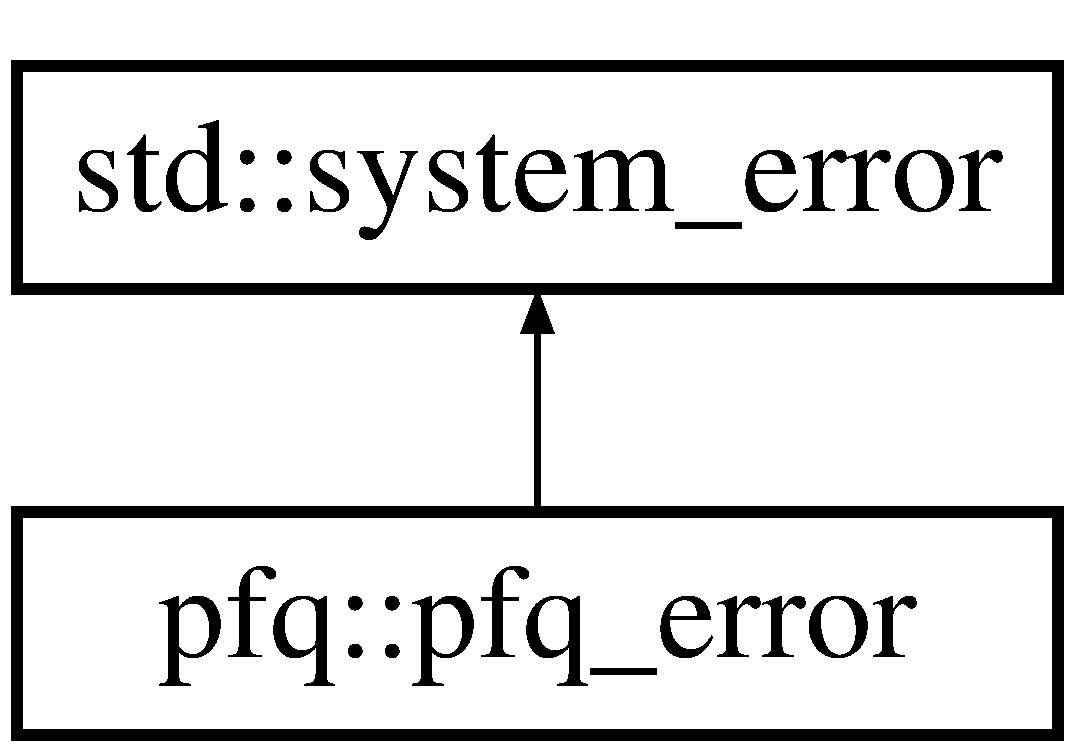
\includegraphics[height=2.000000cm]{classpfq_1_1pfq__error}
\end{center}
\end{figure}
\subsection*{Public Member Functions}
\begin{DoxyCompactItemize}
\item 
\hyperlink{classpfq_1_1pfq__error_af30cff741114b46fd4c50cef987d3ac4}{pfq\+\_\+error} (std\+::string const \&reason)
\item 
\hyperlink{classpfq_1_1pfq__error_ad11ae06da6b581f49d40081d51ae4a6b}{pfq\+\_\+error} (int ev, std\+::string const \&reason)
\item 
\hyperlink{classpfq_1_1pfq__error_a200dca27eee04a6da834364b9342a81d}{pfq\+\_\+error} (int ev, const char $\ast$reason)
\item 
\hyperlink{classpfq_1_1pfq__error_a5af35c9d9dea6aceff0672b92ad6b844}{pfq\+\_\+error} (const char $\ast$reason)
\item 
\hyperlink{classpfq_1_1pfq__error_a64f033ecc5b20bd22872fee3f22fd499}{pfq\+\_\+error} (const \hyperlink{classpfq_1_1pfq__error}{pfq\+\_\+error} \&)=default
\item 
virtual \hyperlink{classpfq_1_1pfq__error_a0aeb73a633e889817967897ef28b3512}{$\sim$pfq\+\_\+error} () noexcept
\end{DoxyCompactItemize}


\subsection{Detailed Description}
Subclass of std\+::system\+\_\+error. 

\hyperlink{classpfq_1_1pfq__error}{pfq\+\_\+error} represent problems related to the P\+F\+Q system. 

\subsection{Constructor \& Destructor Documentation}
\hypertarget{classpfq_1_1pfq__error_af30cff741114b46fd4c50cef987d3ac4}{\index{pfq\+::pfq\+\_\+error@{pfq\+::pfq\+\_\+error}!pfq\+\_\+error@{pfq\+\_\+error}}
\index{pfq\+\_\+error@{pfq\+\_\+error}!pfq\+::pfq\+\_\+error@{pfq\+::pfq\+\_\+error}}
\subsubsection[{pfq\+\_\+error}]{\setlength{\rightskip}{0pt plus 5cm}pfq\+::pfq\+\_\+error\+::pfq\+\_\+error (
\begin{DoxyParamCaption}
\item[{std\+::string const \&}]{reason}
\end{DoxyParamCaption}
)\hspace{0.3cm}{\ttfamily [inline]}}}\label{classpfq_1_1pfq__error_af30cff741114b46fd4c50cef987d3ac4}
\hypertarget{classpfq_1_1pfq__error_ad11ae06da6b581f49d40081d51ae4a6b}{\index{pfq\+::pfq\+\_\+error@{pfq\+::pfq\+\_\+error}!pfq\+\_\+error@{pfq\+\_\+error}}
\index{pfq\+\_\+error@{pfq\+\_\+error}!pfq\+::pfq\+\_\+error@{pfq\+::pfq\+\_\+error}}
\subsubsection[{pfq\+\_\+error}]{\setlength{\rightskip}{0pt plus 5cm}pfq\+::pfq\+\_\+error\+::pfq\+\_\+error (
\begin{DoxyParamCaption}
\item[{int}]{ev, }
\item[{std\+::string const \&}]{reason}
\end{DoxyParamCaption}
)\hspace{0.3cm}{\ttfamily [inline]}}}\label{classpfq_1_1pfq__error_ad11ae06da6b581f49d40081d51ae4a6b}
\hypertarget{classpfq_1_1pfq__error_a200dca27eee04a6da834364b9342a81d}{\index{pfq\+::pfq\+\_\+error@{pfq\+::pfq\+\_\+error}!pfq\+\_\+error@{pfq\+\_\+error}}
\index{pfq\+\_\+error@{pfq\+\_\+error}!pfq\+::pfq\+\_\+error@{pfq\+::pfq\+\_\+error}}
\subsubsection[{pfq\+\_\+error}]{\setlength{\rightskip}{0pt plus 5cm}pfq\+::pfq\+\_\+error\+::pfq\+\_\+error (
\begin{DoxyParamCaption}
\item[{int}]{ev, }
\item[{const char $\ast$}]{reason}
\end{DoxyParamCaption}
)\hspace{0.3cm}{\ttfamily [inline]}}}\label{classpfq_1_1pfq__error_a200dca27eee04a6da834364b9342a81d}
\hypertarget{classpfq_1_1pfq__error_a5af35c9d9dea6aceff0672b92ad6b844}{\index{pfq\+::pfq\+\_\+error@{pfq\+::pfq\+\_\+error}!pfq\+\_\+error@{pfq\+\_\+error}}
\index{pfq\+\_\+error@{pfq\+\_\+error}!pfq\+::pfq\+\_\+error@{pfq\+::pfq\+\_\+error}}
\subsubsection[{pfq\+\_\+error}]{\setlength{\rightskip}{0pt plus 5cm}pfq\+::pfq\+\_\+error\+::pfq\+\_\+error (
\begin{DoxyParamCaption}
\item[{const char $\ast$}]{reason}
\end{DoxyParamCaption}
)\hspace{0.3cm}{\ttfamily [inline]}}}\label{classpfq_1_1pfq__error_a5af35c9d9dea6aceff0672b92ad6b844}
\hypertarget{classpfq_1_1pfq__error_a64f033ecc5b20bd22872fee3f22fd499}{\index{pfq\+::pfq\+\_\+error@{pfq\+::pfq\+\_\+error}!pfq\+\_\+error@{pfq\+\_\+error}}
\index{pfq\+\_\+error@{pfq\+\_\+error}!pfq\+::pfq\+\_\+error@{pfq\+::pfq\+\_\+error}}
\subsubsection[{pfq\+\_\+error}]{\setlength{\rightskip}{0pt plus 5cm}pfq\+::pfq\+\_\+error\+::pfq\+\_\+error (
\begin{DoxyParamCaption}
\item[{const {\bf pfq\+\_\+error} \&}]{}
\end{DoxyParamCaption}
)\hspace{0.3cm}{\ttfamily [default]}}}\label{classpfq_1_1pfq__error_a64f033ecc5b20bd22872fee3f22fd499}
\hypertarget{classpfq_1_1pfq__error_a0aeb73a633e889817967897ef28b3512}{\index{pfq\+::pfq\+\_\+error@{pfq\+::pfq\+\_\+error}!````~pfq\+\_\+error@{$\sim$pfq\+\_\+error}}
\index{````~pfq\+\_\+error@{$\sim$pfq\+\_\+error}!pfq\+::pfq\+\_\+error@{pfq\+::pfq\+\_\+error}}
\subsubsection[{$\sim$pfq\+\_\+error}]{\setlength{\rightskip}{0pt plus 5cm}virtual pfq\+::pfq\+\_\+error\+::$\sim$pfq\+\_\+error (
\begin{DoxyParamCaption}
{}
\end{DoxyParamCaption}
)\hspace{0.3cm}{\ttfamily [inline]}, {\ttfamily [virtual]}, {\ttfamily [noexcept]}}}\label{classpfq_1_1pfq__error_a0aeb73a633e889817967897ef28b3512}


The documentation for this class was generated from the following file\+:\begin{DoxyCompactItemize}
\item 
C++/pfq/\hyperlink{exception_8hpp}{exception.\+hpp}\end{DoxyCompactItemize}

\hypertarget{structpfq_1_1param_1_1policy}{}\section{pfq\+:\+:param\+:\+:policy Struct Reference}
\label{structpfq_1_1param_1_1policy}\index{pfq\+::param\+::policy@{pfq\+::param\+::policy}}


{\ttfamily \#include $<$pfq.\+hpp$>$}

\subsection*{Public Attributes}
\begin{DoxyCompactItemize}
\item 
\hyperlink{namespacepfq_ac41249c8510558905b01fa4d866a38d7}{group\+\_\+policy} \hyperlink{structpfq_1_1param_1_1policy_ab0e84b461546b9e889dbe7b56ae39cdf}{value}
\end{DoxyCompactItemize}


\subsection{Member Data Documentation}
\mbox{\Hypertarget{structpfq_1_1param_1_1policy_ab0e84b461546b9e889dbe7b56ae39cdf}\label{structpfq_1_1param_1_1policy_ab0e84b461546b9e889dbe7b56ae39cdf}} 
\index{pfq\+::param\+::policy@{pfq\+::param\+::policy}!value@{value}}
\index{value@{value}!pfq\+::param\+::policy@{pfq\+::param\+::policy}}
\subsubsection{\texorpdfstring{value}{value}}
{\footnotesize\ttfamily \hyperlink{namespacepfq_ac41249c8510558905b01fa4d866a38d7}{group\+\_\+policy} pfq\+::param\+::policy\+::value}



The documentation for this struct was generated from the following file\+:\begin{DoxyCompactItemize}
\item 
C++/pfq/\hyperlink{pfq_8hpp}{pfq.\+hpp}\end{DoxyCompactItemize}

\hypertarget{structpfq_1_1param_1_1rx__slots}{}\section{pfq\+:\+:param\+:\+:rx\+\_\+slots Struct Reference}
\label{structpfq_1_1param_1_1rx__slots}\index{pfq\+::param\+::rx\+\_\+slots@{pfq\+::param\+::rx\+\_\+slots}}


{\ttfamily \#include $<$pfq.\+hpp$>$}

\subsection*{Public Attributes}
\begin{DoxyCompactItemize}
\item 
size\+\_\+t \hyperlink{structpfq_1_1param_1_1rx__slots_a2bafbed5d322cf89df33ca10bc397822}{value}
\end{DoxyCompactItemize}


\subsection{Member Data Documentation}
\mbox{\Hypertarget{structpfq_1_1param_1_1rx__slots_a2bafbed5d322cf89df33ca10bc397822}\label{structpfq_1_1param_1_1rx__slots_a2bafbed5d322cf89df33ca10bc397822}} 
\index{pfq\+::param\+::rx\+\_\+slots@{pfq\+::param\+::rx\+\_\+slots}!value@{value}}
\index{value@{value}!pfq\+::param\+::rx\+\_\+slots@{pfq\+::param\+::rx\+\_\+slots}}
\subsubsection{\texorpdfstring{value}{value}}
{\footnotesize\ttfamily size\+\_\+t pfq\+::param\+::rx\+\_\+slots\+::value}



The documentation for this struct was generated from the following file\+:\begin{DoxyCompactItemize}
\item 
C++/pfq/\hyperlink{pfq_8hpp}{pfq.\+hpp}\end{DoxyCompactItemize}

\hypertarget{classpfq_1_1socket}{\section{pfq\+:\+:socket Class Reference}
\label{classpfq_1_1socket}\index{pfq\+::socket@{pfq\+::socket}}
}


P\+F\+Q\+: the socket.  




{\ttfamily \#include $<$pfq.\+hpp$>$}

\subsection*{Public Member Functions}
\begin{DoxyCompactItemize}
\item 
\hyperlink{classpfq_1_1socket_a169a46cd01a5fd0a71919ece48f18d9d}{socket} ()
\begin{DoxyCompactList}\small\item\em Default constructor. \end{DoxyCompactList}\item 
{\footnotesize template$<$typename... Ts$>$ }\\\hyperlink{classpfq_1_1socket_aa53695f39b45a0fa9520d52a1a35d2bf}{socket} (param\+::list\+\_\+t, Ts \&\&...args)
\begin{DoxyCompactList}\small\item\em Constructor with named-\/parameter idiom (\hyperlink{namespacepfq_1_1param_a09da2abc1a228d7f77c35bed3bdb157d}{param\+::get} is the C++14 std\+::get) \end{DoxyCompactList}\item 
\hyperlink{classpfq_1_1socket_ae1799cb604036f836299a1dd5b0c2ef7}{socket} (size\+\_\+t \hyperlink{classpfq_1_1socket_ab68dbba5ef01041b9c96758c4a9f0a6c}{caplen}, size\+\_\+t \hyperlink{classpfq_1_1socket_a5cf700fc12d67b91df3d669ac4aa737a}{rx\+\_\+slots}=65536, size\+\_\+t \hyperlink{classpfq_1_1socket_a863da5015c00d6a49f1515b703c24230}{maxlen}=64, size\+\_\+t \hyperlink{classpfq_1_1socket_a019d15a072c043d6a1333ca0c836da4c}{tx\+\_\+slots}=4096)
\begin{DoxyCompactList}\small\item\em Constructor. \end{DoxyCompactList}\item 
\hyperlink{classpfq_1_1socket_a768f20e043a2244dcb0f88d03120b28a}{socket} (\hyperlink{namespacepfq_ac41249c8510558905b01fa4d866a38d7}{group\+\_\+policy} policy, size\+\_\+t \hyperlink{classpfq_1_1socket_ab68dbba5ef01041b9c96758c4a9f0a6c}{caplen}, size\+\_\+t \hyperlink{classpfq_1_1socket_a5cf700fc12d67b91df3d669ac4aa737a}{rx\+\_\+slots}=65536, size\+\_\+t \hyperlink{classpfq_1_1socket_a863da5015c00d6a49f1515b703c24230}{maxlen}=64, size\+\_\+t \hyperlink{classpfq_1_1socket_a019d15a072c043d6a1333ca0c836da4c}{tx\+\_\+slots}=4096)
\begin{DoxyCompactList}\small\item\em Constructor. \end{DoxyCompactList}\item 
\hyperlink{classpfq_1_1socket_a9aa326dac10a561a5bffadeffb928179}{socket} (\hyperlink{namespacepfq_a96af1f5ed530eff563eb917516758fbb}{class\+\_\+mask} mask, \hyperlink{namespacepfq_ac41249c8510558905b01fa4d866a38d7}{group\+\_\+policy} policy, size\+\_\+t \hyperlink{classpfq_1_1socket_ab68dbba5ef01041b9c96758c4a9f0a6c}{caplen}, size\+\_\+t \hyperlink{classpfq_1_1socket_a5cf700fc12d67b91df3d669ac4aa737a}{rx\+\_\+slots}=65536, size\+\_\+t \hyperlink{classpfq_1_1socket_a863da5015c00d6a49f1515b703c24230}{maxlen}=64, size\+\_\+t \hyperlink{classpfq_1_1socket_a019d15a072c043d6a1333ca0c836da4c}{tx\+\_\+slots}=4096)
\begin{DoxyCompactList}\small\item\em Constructor. \end{DoxyCompactList}\item 
\hyperlink{classpfq_1_1socket_a08fbdcc1736de36d205282ce20ffbaa3}{$\sim$socket} ()
\begin{DoxyCompactList}\small\item\em Destructor\+: close the socket. \end{DoxyCompactList}\item 
\hyperlink{classpfq_1_1socket_a517b6fdd622cdb2a64f2960176296f8d}{socket} (const \hyperlink{classpfq_1_1socket}{socket} \&)=delete
\begin{DoxyCompactList}\small\item\em P\+F\+Q socket is a non-\/copyable resource. \end{DoxyCompactList}\item 
\hyperlink{classpfq_1_1socket}{socket} \& \hyperlink{classpfq_1_1socket_a3cfd9674358a2ffd8b37e76d73b8a654}{operator=} (const \hyperlink{classpfq_1_1socket}{socket} \&)=delete
\begin{DoxyCompactList}\small\item\em P\+F\+Q socket is a non-\/copy assignable resource. \end{DoxyCompactList}\item 
\hyperlink{classpfq_1_1socket_a1a60820551f1601beb54649d9ae48fa2}{socket} (\hyperlink{classpfq_1_1socket}{socket} \&\&other) noexcept
\begin{DoxyCompactList}\small\item\em Move constructor. \end{DoxyCompactList}\item 
\hyperlink{classpfq_1_1socket}{socket} \& \hyperlink{classpfq_1_1socket_a8022eafa68b84a840292ebcfc4d1ba7a}{operator=} (\hyperlink{classpfq_1_1socket}{socket} \&\&other) noexcept
\begin{DoxyCompactList}\small\item\em Move assignment operator. \end{DoxyCompactList}\item 
void \hyperlink{classpfq_1_1socket_ac80ebddf3a94f7964c74bf02954704ce}{swap} (\hyperlink{classpfq_1_1socket}{socket} \&other)
\begin{DoxyCompactList}\small\item\em Swap two P\+F\+Q sockets. \end{DoxyCompactList}\item 
void \hyperlink{classpfq_1_1socket_a4e9f7b3dfcf771163995fc10ed8835f8}{open} (\hyperlink{namespacepfq_ac41249c8510558905b01fa4d866a38d7}{group\+\_\+policy} policy, size\+\_\+t \hyperlink{classpfq_1_1socket_ab68dbba5ef01041b9c96758c4a9f0a6c}{caplen}, size\+\_\+t \hyperlink{classpfq_1_1socket_a5cf700fc12d67b91df3d669ac4aa737a}{rx\+\_\+slots}=65536, size\+\_\+t \hyperlink{classpfq_1_1socket_a863da5015c00d6a49f1515b703c24230}{maxlen}=64, size\+\_\+t \hyperlink{classpfq_1_1socket_a019d15a072c043d6a1333ca0c836da4c}{tx\+\_\+slots}=4096)
\begin{DoxyCompactList}\small\item\em Open the P\+F\+Q socket with the given group policy. \end{DoxyCompactList}\item 
void \hyperlink{classpfq_1_1socket_a4c622a6debdcae9cfae0abb30c47678c}{open} (\hyperlink{namespacepfq_a96af1f5ed530eff563eb917516758fbb}{class\+\_\+mask} mask, \hyperlink{namespacepfq_ac41249c8510558905b01fa4d866a38d7}{group\+\_\+policy} policy, size\+\_\+t \hyperlink{classpfq_1_1socket_ab68dbba5ef01041b9c96758c4a9f0a6c}{caplen}, size\+\_\+t \hyperlink{classpfq_1_1socket_a5cf700fc12d67b91df3d669ac4aa737a}{rx\+\_\+slots}=65536, size\+\_\+t \hyperlink{classpfq_1_1socket_a863da5015c00d6a49f1515b703c24230}{maxlen}=64, size\+\_\+t \hyperlink{classpfq_1_1socket_a019d15a072c043d6a1333ca0c836da4c}{tx\+\_\+slots}=4096)
\begin{DoxyCompactList}\small\item\em Open the P\+F\+Q socket with the given class mask and group policy. \end{DoxyCompactList}\item 
{\footnotesize template$<$typename... Ts$>$ }\\void \hyperlink{classpfq_1_1socket_a33c3e305c62f5a9f8a0ef74f69097ecf}{open} (param\+::list\+\_\+t, Ts \&\&...args)
\begin{DoxyCompactList}\small\item\em Open the socket with named-\/parameter idiom. \end{DoxyCompactList}\item 
int \hyperlink{classpfq_1_1socket_af3f79e9a42964907acd581d35d42da00}{id} () const 
\begin{DoxyCompactList}\small\item\em Return the id for the socket. \end{DoxyCompactList}\item 
int \hyperlink{classpfq_1_1socket_a0b82186997f22efffd336b09b19a806d}{group\+\_\+id} () const 
\begin{DoxyCompactList}\small\item\em Return the group-\/id for the socket. \end{DoxyCompactList}\item 
int \hyperlink{classpfq_1_1socket_ad4f1a171d31215afd6aad769a5e4b004}{fd} () const 
\begin{DoxyCompactList}\small\item\em Return the underlying file descriptor. \end{DoxyCompactList}\item 
void \hyperlink{classpfq_1_1socket_a4c179188ea8fceeb5fd47d52f93c6bda}{close} ()
\begin{DoxyCompactList}\small\item\em Close the socket. \end{DoxyCompactList}\item 
void \hyperlink{classpfq_1_1socket_a5b25af762946405695f4192b08c04146}{enable} ()
\begin{DoxyCompactList}\small\item\em Enable the socket for packet capture. \end{DoxyCompactList}\item 
void \hyperlink{classpfq_1_1socket_ac7e918bff7d1672125a8549dae750dcc}{disable} ()
\begin{DoxyCompactList}\small\item\em Disable the packet capture. \end{DoxyCompactList}\item 
bool \hyperlink{classpfq_1_1socket_acec42300a779676e326844209c1c0948}{enabled} () const 
\begin{DoxyCompactList}\small\item\em Check whether the packet capture is enabled. \end{DoxyCompactList}\item 
void \hyperlink{classpfq_1_1socket_ab21f7cd8d22e57ec28b3038d259561bc}{timestamp\+\_\+enable} (bool value)
\begin{DoxyCompactList}\small\item\em Set the timestamping for packets. \end{DoxyCompactList}\item 
bool \hyperlink{classpfq_1_1socket_a6a170b8ebc6b03760c4096cd176af8cf}{timestamp\+\_\+enabled} () const 
\begin{DoxyCompactList}\small\item\em Check whether the timestamping is enabled for packets. \end{DoxyCompactList}\item 
void \hyperlink{classpfq_1_1socket_ab68dbba5ef01041b9c96758c4a9f0a6c}{caplen} (size\+\_\+t value)
\begin{DoxyCompactList}\small\item\em Specify the capture length of packets, in bytes. \end{DoxyCompactList}\item 
size\+\_\+t \hyperlink{classpfq_1_1socket_a768bee4d974acdc5ee9ee879b0903c54}{caplen} () const 
\begin{DoxyCompactList}\small\item\em Return the capture length of packets, in bytes. \end{DoxyCompactList}\item 
void \hyperlink{classpfq_1_1socket_a863da5015c00d6a49f1515b703c24230}{maxlen} (size\+\_\+t value)
\begin{DoxyCompactList}\small\item\em Specify the max transmission length of packets, in bytes. \end{DoxyCompactList}\item 
size\+\_\+t \hyperlink{classpfq_1_1socket_a45bd7aa973fe4eccce899c552adfedb5}{maxlen} () const 
\begin{DoxyCompactList}\small\item\em Return the max transmission length of packets, in bytes. \end{DoxyCompactList}\item 
void \hyperlink{classpfq_1_1socket_a5cf700fc12d67b91df3d669ac4aa737a}{rx\+\_\+slots} (size\+\_\+t value)
\begin{DoxyCompactList}\small\item\em Specify the length of the R\+X queue, in number of packets. \end{DoxyCompactList}\item 
size\+\_\+t \hyperlink{classpfq_1_1socket_a0f2205329249eaa7a6229980a744fd2a}{rx\+\_\+slots} () const 
\begin{DoxyCompactList}\small\item\em Return the length of the R\+X queue, in number of packets. \end{DoxyCompactList}\item 
void \hyperlink{classpfq_1_1socket_a019d15a072c043d6a1333ca0c836da4c}{tx\+\_\+slots} (size\+\_\+t value)
\begin{DoxyCompactList}\small\item\em Specify the length of the T\+X queue, in number of packets. \end{DoxyCompactList}\item 
size\+\_\+t \hyperlink{classpfq_1_1socket_a11b91a39fdae65cace365aa3583eba7d}{tx\+\_\+slots} () const 
\begin{DoxyCompactList}\small\item\em Return the length of the T\+X queue, in number of packets. \end{DoxyCompactList}\item 
size\+\_\+t \hyperlink{classpfq_1_1socket_a8e290b6b1105c22b538d38021d6bfb7d}{rx\+\_\+slot\+\_\+size} () const 
\begin{DoxyCompactList}\small\item\em Return the length of a R\+X slot, in bytes. \end{DoxyCompactList}\item 
void \hyperlink{classpfq_1_1socket_a3a0fc5c70e2d2615e29d06ac55007ed3}{bind} (const char $\ast$dev, int \hyperlink{classpfq_1_1queue}{queue}=any\+\_\+queue)
\begin{DoxyCompactList}\small\item\em Bind the main group of the socket to the given device/queue. \end{DoxyCompactList}\item 
void \hyperlink{classpfq_1_1socket_a4d4d44cc68af0290e3c494dcd10b1541}{bind\+\_\+group} (int gid, const char $\ast$dev, int \hyperlink{classpfq_1_1queue}{queue}=any\+\_\+queue)
\begin{DoxyCompactList}\small\item\em Bind the given group to the given device/queue. \end{DoxyCompactList}\item 
void \hyperlink{classpfq_1_1socket_af53d407f46ba2b4d143782ff7d585758}{unbind} (const char $\ast$dev, int \hyperlink{classpfq_1_1queue}{queue}=any\+\_\+queue)
\begin{DoxyCompactList}\small\item\em Unbind the main group of the socket from the given device/queue. \end{DoxyCompactList}\item 
void \hyperlink{classpfq_1_1socket_a6e1f7ee7f44b6824d734d4ff7046d907}{unbind\+\_\+group} (int gid, const char $\ast$dev, int \hyperlink{classpfq_1_1queue}{queue}=any\+\_\+queue)
\begin{DoxyCompactList}\small\item\em Unbind the given group from the given device/queue. \end{DoxyCompactList}\item 
void \hyperlink{classpfq_1_1socket_a2c96741054ea764f5d8c31295ef5df29}{egress\+\_\+bind} (const char $\ast$dev, int \hyperlink{classpfq_1_1queue}{queue}=any\+\_\+queue)
\begin{DoxyCompactList}\small\item\em Mark the socket as egress and bind it to the given device/queue. \end{DoxyCompactList}\item 
void \hyperlink{classpfq_1_1socket_ae80718e8f26cdaed3fd05bfde6d835e0}{egress\+\_\+unbind} ()
\begin{DoxyCompactList}\small\item\em Unmark the socket as egress. \end{DoxyCompactList}\item 
unsigned long \hyperlink{classpfq_1_1socket_a45c12f4255af4eb74bb9a75d8e1a56eb}{groups\+\_\+mask} () const 
\begin{DoxyCompactList}\small\item\em Return the mask of the joined groups. \end{DoxyCompactList}\item 
std\+::vector$<$ int $>$ \hyperlink{classpfq_1_1socket_a7bb02f670cf9c16b4339f650c7b80de7}{groups} () const 
\begin{DoxyCompactList}\small\item\em Obtain the list of the joined groups. \end{DoxyCompactList}\item 
{\footnotesize template$<$typename Comp $>$ }\\void \hyperlink{classpfq_1_1socket_a5cb37765ffcb1b78c5d61211f9e806df}{set\+\_\+group\+\_\+computation} (int gid, Comp const \&comp)
\begin{DoxyCompactList}\small\item\em Specify a functional computation for the given group. \end{DoxyCompactList}\item 
void \hyperlink{classpfq_1_1socket_acd2ef781a82b49566f03a085ba091138}{set\+\_\+group\+\_\+computation} (int gid, pfq\+\_\+computation\+\_\+descr $\ast$prog)
\begin{DoxyCompactList}\small\item\em Specify a functional computation for the given group. \end{DoxyCompactList}\item 
void \hyperlink{classpfq_1_1socket_a968ae9e3375650990488dcb1784a4bd1}{set\+\_\+group\+\_\+computation} (int gid, std\+::string prog)
\begin{DoxyCompactList}\small\item\em Specify a functional computation for the given group, from string. \end{DoxyCompactList}\item 
void \hyperlink{classpfq_1_1socket_ad618894910a12a08eaed3d8668db25af}{set\+\_\+group\+\_\+fprog} (int gid, const sock\+\_\+fprog \&f)
\begin{DoxyCompactList}\small\item\em Specify a B\+P\+F program for the given group. \end{DoxyCompactList}\item 
void \hyperlink{classpfq_1_1socket_a2327e71a6f94e54efb0da5ec36b1c620}{reset\+\_\+group\+\_\+fprog} (int gid)
\begin{DoxyCompactList}\small\item\em Reset the B\+P\+F program fro the given group. \end{DoxyCompactList}\item 
int \hyperlink{classpfq_1_1socket_afbd75341794fae964ed23ce5858fd153}{join\+\_\+group} (int gid, \hyperlink{namespacepfq_ac41249c8510558905b01fa4d866a38d7}{group\+\_\+policy} pol=\hyperlink{namespacepfq_ac41249c8510558905b01fa4d866a38d7a9e81e7b963c71363e2fb3eefcfecfc0e}{group\+\_\+policy\+::shared}, \hyperlink{namespacepfq_a96af1f5ed530eff563eb917516758fbb}{class\+\_\+mask} mask=\hyperlink{namespacepfq_a96af1f5ed530eff563eb917516758fbba172b03053216c6158fe380805998ad6c}{class\+\_\+mask\+::default\+\_\+})
\begin{DoxyCompactList}\small\item\em Join the given group. \end{DoxyCompactList}\item 
void \hyperlink{classpfq_1_1socket_ac512d6b89db52da73a51ba9112658180}{leave\+\_\+group} (int gid)
\begin{DoxyCompactList}\small\item\em Leave the given group. \end{DoxyCompactList}\item 
int \hyperlink{classpfq_1_1socket_ad8ce551ea07f39317bb383ab88d66344}{poll} (long int microseconds=-\/1)
\begin{DoxyCompactList}\small\item\em Wait for packets. \end{DoxyCompactList}\item 
\hyperlink{classpfq_1_1queue}{queue} \hyperlink{classpfq_1_1socket_a6a79c81d3c366e49b8d64eb828ae5540}{read} (long int microseconds=-\/1)
\begin{DoxyCompactList}\small\item\em Read packets in place. \end{DoxyCompactList}\item 
uint8\+\_\+t \hyperlink{classpfq_1_1socket_aba44de6422e3e10b65474e7f3999ebd0}{current\+\_\+commit} () const 
\begin{DoxyCompactList}\small\item\em Return the current commit version (used internally by the memory mapped queue). \end{DoxyCompactList}\item 
\hyperlink{classpfq_1_1queue}{queue} \hyperlink{classpfq_1_1socket_ace69fbf64216b7b30a8a305a9d25229b}{recv} (const \hyperlink{namespacepfq_ad7b88920eaf729154354741132483ea8}{mutable\+\_\+buffer} \&buff, long int microseconds=-\/1)
\begin{DoxyCompactList}\small\item\em Receive packets in the given mutable buffer. \end{DoxyCompactList}\item 
{\footnotesize template$<$typename Fun $>$ }\\size\+\_\+t \hyperlink{classpfq_1_1socket_ae6cd08be2e7c35a548a64fded4359612}{dispatch} (Fun callback, long int microseconds=-\/1, char $\ast$user=nullptr)
\begin{DoxyCompactList}\small\item\em This function takes an instance of a callable type which is invoked on each packet captured. \end{DoxyCompactList}\item 
void \hyperlink{classpfq_1_1socket_aaf91b2e089edb2c4695584b01774326e}{vlan\+\_\+filters\+\_\+enable} (int gid, bool toggle)
\begin{DoxyCompactList}\small\item\em Set vlan filtering for the given group. \end{DoxyCompactList}\item 
void \hyperlink{classpfq_1_1socket_a92eeaf78ff595546c517b5699c9a5b1e}{vlan\+\_\+set\+\_\+filter} (int gid, int vid)
\begin{DoxyCompactList}\small\item\em Specify a capture filter for the given group and vlan id. \end{DoxyCompactList}\item 
{\footnotesize template$<$typename Iter $>$ }\\void \hyperlink{classpfq_1_1socket_aee0fbc6a5f899d081c659dbaa4a4a235}{vlan\+\_\+set\+\_\+filter} (int gid, Iter beg, Iter end)
\begin{DoxyCompactList}\small\item\em Specify the vlan capture filters in the given range. \end{DoxyCompactList}\item 
void \hyperlink{classpfq_1_1socket_a296d1eddfb061c1a658067006ddb9f37}{vlan\+\_\+reset\+\_\+filter} (int gid, int vid)
\begin{DoxyCompactList}\small\item\em Reset all vlan filters. \end{DoxyCompactList}\item 
{\footnotesize template$<$typename Iter $>$ }\\void \hyperlink{classpfq_1_1socket_a18efa89248a6d6bfb29d575744d21608}{vlan\+\_\+reset\+\_\+filter} (int gid, Iter beg, Iter end)
\begin{DoxyCompactList}\small\item\em Reset the vlan id filters specified in the given range. \end{DoxyCompactList}\item 
pfq\+\_\+stats \hyperlink{classpfq_1_1socket_a0a0a637d733613bf86d6d85168d2e37f}{stats} () const 
\begin{DoxyCompactList}\small\item\em Return the socket stats. \end{DoxyCompactList}\item 
pfq\+\_\+stats \hyperlink{classpfq_1_1socket_a39397866032a4654c4dc000185c61e01}{group\+\_\+stats} (int gid) const 
\begin{DoxyCompactList}\small\item\em Return the stats of the given group. \end{DoxyCompactList}\item 
std\+::vector$<$ unsigned long $>$ \hyperlink{classpfq_1_1socket_a5bb4734939ffeb151e199182ec30c4de}{group\+\_\+counters} (int gid) const 
\begin{DoxyCompactList}\small\item\em Return the counters of the given group. \end{DoxyCompactList}\item 
size\+\_\+t \hyperlink{classpfq_1_1socket_a1888ae33a42258fdbb2aac1dc3feb55c}{mem\+\_\+size} () const 
\begin{DoxyCompactList}\small\item\em Return the memory size of the R\+X queue. \end{DoxyCompactList}\item 
const void $\ast$ \hyperlink{classpfq_1_1socket_a32275b5b77913fadc7671efdef75369b}{mem\+\_\+addr} () const 
\begin{DoxyCompactList}\small\item\em Return the address of the R\+X queue. \end{DoxyCompactList}\item 
void \hyperlink{classpfq_1_1socket_a986a4bb8c7b23fd73ce1e8f340a3fb67}{bind\+\_\+tx} (const char $\ast$dev, int \hyperlink{classpfq_1_1queue}{queue}=any\+\_\+queue)
\begin{DoxyCompactList}\small\item\em Bind the socket for transmission to the given device name and queue. \end{DoxyCompactList}\item 
bool \hyperlink{classpfq_1_1socket_ab0b61a0a5741e24aa7cfbf090e2dc776}{send} (\hyperlink{namespacepfq_ac835a1bd09b4cbaba61c100b50d0a99f}{const\+\_\+buffer} pkt)
\begin{DoxyCompactList}\small\item\em Transmit the packet stored in the given buffer. \end{DoxyCompactList}\item 
bool \hyperlink{classpfq_1_1socket_a73acb3e9a0ee657255385c32ef53334e}{send\+\_\+sync} (\hyperlink{namespacepfq_ac835a1bd09b4cbaba61c100b50d0a99f}{const\+\_\+buffer} pkt, size\+\_\+t n=128)
\begin{DoxyCompactList}\small\item\em Store the packet and possibly transmit the packets in the queue, synchronously. \end{DoxyCompactList}\item 
bool \hyperlink{classpfq_1_1socket_a7def045b0472dc611c95c80f512c6e7e}{send\+\_\+async} (\hyperlink{namespacepfq_ac835a1bd09b4cbaba61c100b50d0a99f}{const\+\_\+buffer} pkt, size\+\_\+t n=128)
\begin{DoxyCompactList}\small\item\em Store the packet and possibly transmit the packets in the queue, asynchronously. \end{DoxyCompactList}\item 
bool \hyperlink{classpfq_1_1socket_ae237165f4533990f1e39386235b2e72c}{inject} (\hyperlink{namespacepfq_ac835a1bd09b4cbaba61c100b50d0a99f}{const\+\_\+buffer} pkt)
\begin{DoxyCompactList}\small\item\em Schedule the packet for transmission. \end{DoxyCompactList}\item 
void \hyperlink{classpfq_1_1socket_a29a751a6e0f547bac18c8d812be6224f}{start\+\_\+tx\+\_\+thread} (int node)
\begin{DoxyCompactList}\small\item\em Start the T\+X kernel thread. \end{DoxyCompactList}\item 
void \hyperlink{classpfq_1_1socket_a4aefc5e4af5aa36ada44bda78499b642}{stop\+\_\+tx\+\_\+thread} ()
\begin{DoxyCompactList}\small\item\em Stop the T\+X kernel thread. \end{DoxyCompactList}\item 
void \hyperlink{classpfq_1_1socket_aa77904b5b7cee56663f3e3acaad6cfd7}{wakeup\+\_\+tx\+\_\+thread} ()
\begin{DoxyCompactList}\small\item\em Wakeup the T\+X kernel thread. \end{DoxyCompactList}\item 
void \hyperlink{classpfq_1_1socket_a62c065ee5725e03aa2912d0d2ea893de}{tx\+\_\+queue\+\_\+flush} ()
\begin{DoxyCompactList}\small\item\em Flush the T\+X queue, in the context of the calling thread. \end{DoxyCompactList}\end{DoxyCompactItemize}


\subsection{Detailed Description}
P\+F\+Q\+: the socket. 

This class is the main interface to the P\+F\+Q kernel module. Each instance handles a socket that can be used to receive from and transmit packets to the network. 

\subsection{Constructor \& Destructor Documentation}
\hypertarget{classpfq_1_1socket_a169a46cd01a5fd0a71919ece48f18d9d}{\index{pfq\+::socket@{pfq\+::socket}!socket@{socket}}
\index{socket@{socket}!pfq\+::socket@{pfq\+::socket}}
\subsubsection[{socket}]{\setlength{\rightskip}{0pt plus 5cm}pfq\+::socket\+::socket (
\begin{DoxyParamCaption}
{}
\end{DoxyParamCaption}
)\hspace{0.3cm}{\ttfamily [inline]}}}\label{classpfq_1_1socket_a169a46cd01a5fd0a71919ece48f18d9d}


Default constructor. 

\hypertarget{classpfq_1_1socket_aa53695f39b45a0fa9520d52a1a35d2bf}{\index{pfq\+::socket@{pfq\+::socket}!socket@{socket}}
\index{socket@{socket}!pfq\+::socket@{pfq\+::socket}}
\subsubsection[{socket}]{\setlength{\rightskip}{0pt plus 5cm}template$<$typename... Ts$>$ pfq\+::socket\+::socket (
\begin{DoxyParamCaption}
\item[{param\+::list\+\_\+t}]{, }
\item[{Ts \&\&...}]{args}
\end{DoxyParamCaption}
)\hspace{0.3cm}{\ttfamily [inline]}}}\label{classpfq_1_1socket_aa53695f39b45a0fa9520d52a1a35d2bf}


Constructor with named-\/parameter idiom (\hyperlink{namespacepfq_1_1param_a09da2abc1a228d7f77c35bed3bdb157d}{param\+::get} is the C++14 std\+::get) 

\hypertarget{classpfq_1_1socket_ae1799cb604036f836299a1dd5b0c2ef7}{\index{pfq\+::socket@{pfq\+::socket}!socket@{socket}}
\index{socket@{socket}!pfq\+::socket@{pfq\+::socket}}
\subsubsection[{socket}]{\setlength{\rightskip}{0pt plus 5cm}pfq\+::socket\+::socket (
\begin{DoxyParamCaption}
\item[{size\+\_\+t}]{caplen, }
\item[{size\+\_\+t}]{rx\+\_\+slots = {\ttfamily 65536}, }
\item[{size\+\_\+t}]{maxlen = {\ttfamily 64}, }
\item[{size\+\_\+t}]{tx\+\_\+slots = {\ttfamily 4096}}
\end{DoxyParamCaption}
)\hspace{0.3cm}{\ttfamily [inline]}}}\label{classpfq_1_1socket_ae1799cb604036f836299a1dd5b0c2ef7}


Constructor. 

Create a P\+F\+Q socket and join a new group. \hypertarget{classpfq_1_1socket_a768f20e043a2244dcb0f88d03120b28a}{\index{pfq\+::socket@{pfq\+::socket}!socket@{socket}}
\index{socket@{socket}!pfq\+::socket@{pfq\+::socket}}
\subsubsection[{socket}]{\setlength{\rightskip}{0pt plus 5cm}pfq\+::socket\+::socket (
\begin{DoxyParamCaption}
\item[{{\bf group\+\_\+policy}}]{policy, }
\item[{size\+\_\+t}]{caplen, }
\item[{size\+\_\+t}]{rx\+\_\+slots = {\ttfamily 65536}, }
\item[{size\+\_\+t}]{maxlen = {\ttfamily 64}, }
\item[{size\+\_\+t}]{tx\+\_\+slots = {\ttfamily 4096}}
\end{DoxyParamCaption}
)\hspace{0.3cm}{\ttfamily [inline]}}}\label{classpfq_1_1socket_a768f20e043a2244dcb0f88d03120b28a}


Constructor. 

Create a P\+F\+Q socket with the given group policy (default class). \hypertarget{classpfq_1_1socket_a9aa326dac10a561a5bffadeffb928179}{\index{pfq\+::socket@{pfq\+::socket}!socket@{socket}}
\index{socket@{socket}!pfq\+::socket@{pfq\+::socket}}
\subsubsection[{socket}]{\setlength{\rightskip}{0pt plus 5cm}pfq\+::socket\+::socket (
\begin{DoxyParamCaption}
\item[{{\bf class\+\_\+mask}}]{mask, }
\item[{{\bf group\+\_\+policy}}]{policy, }
\item[{size\+\_\+t}]{caplen, }
\item[{size\+\_\+t}]{rx\+\_\+slots = {\ttfamily 65536}, }
\item[{size\+\_\+t}]{maxlen = {\ttfamily 64}, }
\item[{size\+\_\+t}]{tx\+\_\+slots = {\ttfamily 4096}}
\end{DoxyParamCaption}
)\hspace{0.3cm}{\ttfamily [inline]}}}\label{classpfq_1_1socket_a9aa326dac10a561a5bffadeffb928179}


Constructor. 

Create a P\+F\+Q socket with the given class mask and group policy. \hypertarget{classpfq_1_1socket_a08fbdcc1736de36d205282ce20ffbaa3}{\index{pfq\+::socket@{pfq\+::socket}!````~socket@{$\sim$socket}}
\index{````~socket@{$\sim$socket}!pfq\+::socket@{pfq\+::socket}}
\subsubsection[{$\sim$socket}]{\setlength{\rightskip}{0pt plus 5cm}pfq\+::socket\+::$\sim$socket (
\begin{DoxyParamCaption}
{}
\end{DoxyParamCaption}
)\hspace{0.3cm}{\ttfamily [inline]}}}\label{classpfq_1_1socket_a08fbdcc1736de36d205282ce20ffbaa3}


Destructor\+: close the socket. 

\hypertarget{classpfq_1_1socket_a517b6fdd622cdb2a64f2960176296f8d}{\index{pfq\+::socket@{pfq\+::socket}!socket@{socket}}
\index{socket@{socket}!pfq\+::socket@{pfq\+::socket}}
\subsubsection[{socket}]{\setlength{\rightskip}{0pt plus 5cm}pfq\+::socket\+::socket (
\begin{DoxyParamCaption}
\item[{const {\bf socket} \&}]{}
\end{DoxyParamCaption}
)\hspace{0.3cm}{\ttfamily [delete]}}}\label{classpfq_1_1socket_a517b6fdd622cdb2a64f2960176296f8d}


P\+F\+Q socket is a non-\/copyable resource. 

\hypertarget{classpfq_1_1socket_a1a60820551f1601beb54649d9ae48fa2}{\index{pfq\+::socket@{pfq\+::socket}!socket@{socket}}
\index{socket@{socket}!pfq\+::socket@{pfq\+::socket}}
\subsubsection[{socket}]{\setlength{\rightskip}{0pt plus 5cm}pfq\+::socket\+::socket (
\begin{DoxyParamCaption}
\item[{{\bf socket} \&\&}]{other}
\end{DoxyParamCaption}
)\hspace{0.3cm}{\ttfamily [inline]}, {\ttfamily [noexcept]}}}\label{classpfq_1_1socket_a1a60820551f1601beb54649d9ae48fa2}


Move constructor. 



\subsection{Member Function Documentation}
\hypertarget{classpfq_1_1socket_a3a0fc5c70e2d2615e29d06ac55007ed3}{\index{pfq\+::socket@{pfq\+::socket}!bind@{bind}}
\index{bind@{bind}!pfq\+::socket@{pfq\+::socket}}
\subsubsection[{bind}]{\setlength{\rightskip}{0pt plus 5cm}void pfq\+::socket\+::bind (
\begin{DoxyParamCaption}
\item[{const char $\ast$}]{dev, }
\item[{int}]{queue = {\ttfamily any\+\_\+queue}}
\end{DoxyParamCaption}
)\hspace{0.3cm}{\ttfamily [inline]}}}\label{classpfq_1_1socket_a3a0fc5c70e2d2615e29d06ac55007ed3}


Bind the main group of the socket to the given device/queue. 

The first argument is the name of the device; the second argument is the queue number or any\+\_\+queue. \hypertarget{classpfq_1_1socket_a4d4d44cc68af0290e3c494dcd10b1541}{\index{pfq\+::socket@{pfq\+::socket}!bind\+\_\+group@{bind\+\_\+group}}
\index{bind\+\_\+group@{bind\+\_\+group}!pfq\+::socket@{pfq\+::socket}}
\subsubsection[{bind\+\_\+group}]{\setlength{\rightskip}{0pt plus 5cm}void pfq\+::socket\+::bind\+\_\+group (
\begin{DoxyParamCaption}
\item[{int}]{gid, }
\item[{const char $\ast$}]{dev, }
\item[{int}]{queue = {\ttfamily any\+\_\+queue}}
\end{DoxyParamCaption}
)\hspace{0.3cm}{\ttfamily [inline]}}}\label{classpfq_1_1socket_a4d4d44cc68af0290e3c494dcd10b1541}


Bind the given group to the given device/queue. 

The first argument is the name of the device; the second argument is the queue number or any\+\_\+queue. \hypertarget{classpfq_1_1socket_a986a4bb8c7b23fd73ce1e8f340a3fb67}{\index{pfq\+::socket@{pfq\+::socket}!bind\+\_\+tx@{bind\+\_\+tx}}
\index{bind\+\_\+tx@{bind\+\_\+tx}!pfq\+::socket@{pfq\+::socket}}
\subsubsection[{bind\+\_\+tx}]{\setlength{\rightskip}{0pt plus 5cm}void pfq\+::socket\+::bind\+\_\+tx (
\begin{DoxyParamCaption}
\item[{const char $\ast$}]{dev, }
\item[{int}]{queue = {\ttfamily any\+\_\+queue}}
\end{DoxyParamCaption}
)\hspace{0.3cm}{\ttfamily [inline]}}}\label{classpfq_1_1socket_a986a4bb8c7b23fd73ce1e8f340a3fb67}


Bind the socket for transmission to the given device name and queue. 

A socket for transmission can be bound to a given device/queue at time. \hypertarget{classpfq_1_1socket_ab68dbba5ef01041b9c96758c4a9f0a6c}{\index{pfq\+::socket@{pfq\+::socket}!caplen@{caplen}}
\index{caplen@{caplen}!pfq\+::socket@{pfq\+::socket}}
\subsubsection[{caplen}]{\setlength{\rightskip}{0pt plus 5cm}void pfq\+::socket\+::caplen (
\begin{DoxyParamCaption}
\item[{size\+\_\+t}]{value}
\end{DoxyParamCaption}
)\hspace{0.3cm}{\ttfamily [inline]}}}\label{classpfq_1_1socket_ab68dbba5ef01041b9c96758c4a9f0a6c}


Specify the capture length of packets, in bytes. 

Capture length must be set before the socket is enabled to capture. \hypertarget{classpfq_1_1socket_a768bee4d974acdc5ee9ee879b0903c54}{\index{pfq\+::socket@{pfq\+::socket}!caplen@{caplen}}
\index{caplen@{caplen}!pfq\+::socket@{pfq\+::socket}}
\subsubsection[{caplen}]{\setlength{\rightskip}{0pt plus 5cm}size\+\_\+t pfq\+::socket\+::caplen (
\begin{DoxyParamCaption}
{}
\end{DoxyParamCaption}
) const\hspace{0.3cm}{\ttfamily [inline]}}}\label{classpfq_1_1socket_a768bee4d974acdc5ee9ee879b0903c54}


Return the capture length of packets, in bytes. 

\hypertarget{classpfq_1_1socket_a4c179188ea8fceeb5fd47d52f93c6bda}{\index{pfq\+::socket@{pfq\+::socket}!close@{close}}
\index{close@{close}!pfq\+::socket@{pfq\+::socket}}
\subsubsection[{close}]{\setlength{\rightskip}{0pt plus 5cm}void pfq\+::socket\+::close (
\begin{DoxyParamCaption}
{}
\end{DoxyParamCaption}
)\hspace{0.3cm}{\ttfamily [inline]}}}\label{classpfq_1_1socket_a4c179188ea8fceeb5fd47d52f93c6bda}


Close the socket. 

\hypertarget{classpfq_1_1socket_aba44de6422e3e10b65474e7f3999ebd0}{\index{pfq\+::socket@{pfq\+::socket}!current\+\_\+commit@{current\+\_\+commit}}
\index{current\+\_\+commit@{current\+\_\+commit}!pfq\+::socket@{pfq\+::socket}}
\subsubsection[{current\+\_\+commit}]{\setlength{\rightskip}{0pt plus 5cm}uint8\+\_\+t pfq\+::socket\+::current\+\_\+commit (
\begin{DoxyParamCaption}
{}
\end{DoxyParamCaption}
) const\hspace{0.3cm}{\ttfamily [inline]}}}\label{classpfq_1_1socket_aba44de6422e3e10b65474e7f3999ebd0}


Return the current commit version (used internally by the memory mapped queue). 

\hypertarget{classpfq_1_1socket_ac7e918bff7d1672125a8549dae750dcc}{\index{pfq\+::socket@{pfq\+::socket}!disable@{disable}}
\index{disable@{disable}!pfq\+::socket@{pfq\+::socket}}
\subsubsection[{disable}]{\setlength{\rightskip}{0pt plus 5cm}void pfq\+::socket\+::disable (
\begin{DoxyParamCaption}
{}
\end{DoxyParamCaption}
)\hspace{0.3cm}{\ttfamily [inline]}}}\label{classpfq_1_1socket_ac7e918bff7d1672125a8549dae750dcc}


Disable the packet capture. 

\hypertarget{classpfq_1_1socket_ae6cd08be2e7c35a548a64fded4359612}{\index{pfq\+::socket@{pfq\+::socket}!dispatch@{dispatch}}
\index{dispatch@{dispatch}!pfq\+::socket@{pfq\+::socket}}
\subsubsection[{dispatch}]{\setlength{\rightskip}{0pt plus 5cm}template$<$typename Fun $>$ size\+\_\+t pfq\+::socket\+::dispatch (
\begin{DoxyParamCaption}
\item[{Fun}]{callback, }
\item[{long int}]{microseconds = {\ttfamily -\/1}, }
\item[{char $\ast$}]{user = {\ttfamily nullptr}}
\end{DoxyParamCaption}
)\hspace{0.3cm}{\ttfamily [inline]}}}\label{classpfq_1_1socket_ae6cd08be2e7c35a548a64fded4359612}


This function takes an instance of a callable type which is invoked on each packet captured. 

The object must provide the following callable signature\+:

typedef void ($\ast$pfq\+\_\+handler)(char $\ast$user, const struct pfq\+\_\+pkt\+\_\+hdr $\ast$h, const char $\ast$data); \hypertarget{classpfq_1_1socket_a2c96741054ea764f5d8c31295ef5df29}{\index{pfq\+::socket@{pfq\+::socket}!egress\+\_\+bind@{egress\+\_\+bind}}
\index{egress\+\_\+bind@{egress\+\_\+bind}!pfq\+::socket@{pfq\+::socket}}
\subsubsection[{egress\+\_\+bind}]{\setlength{\rightskip}{0pt plus 5cm}void pfq\+::socket\+::egress\+\_\+bind (
\begin{DoxyParamCaption}
\item[{const char $\ast$}]{dev, }
\item[{int}]{queue = {\ttfamily any\+\_\+queue}}
\end{DoxyParamCaption}
)\hspace{0.3cm}{\ttfamily [inline]}}}\label{classpfq_1_1socket_a2c96741054ea764f5d8c31295ef5df29}


Mark the socket as egress and bind it to the given device/queue. 

The egress socket will be used within the capture groups as forwarder. \hypertarget{classpfq_1_1socket_ae80718e8f26cdaed3fd05bfde6d835e0}{\index{pfq\+::socket@{pfq\+::socket}!egress\+\_\+unbind@{egress\+\_\+unbind}}
\index{egress\+\_\+unbind@{egress\+\_\+unbind}!pfq\+::socket@{pfq\+::socket}}
\subsubsection[{egress\+\_\+unbind}]{\setlength{\rightskip}{0pt plus 5cm}void pfq\+::socket\+::egress\+\_\+unbind (
\begin{DoxyParamCaption}
{}
\end{DoxyParamCaption}
)\hspace{0.3cm}{\ttfamily [inline]}}}\label{classpfq_1_1socket_ae80718e8f26cdaed3fd05bfde6d835e0}


Unmark the socket as egress. 

\hypertarget{classpfq_1_1socket_a5b25af762946405695f4192b08c04146}{\index{pfq\+::socket@{pfq\+::socket}!enable@{enable}}
\index{enable@{enable}!pfq\+::socket@{pfq\+::socket}}
\subsubsection[{enable}]{\setlength{\rightskip}{0pt plus 5cm}void pfq\+::socket\+::enable (
\begin{DoxyParamCaption}
{}
\end{DoxyParamCaption}
)\hspace{0.3cm}{\ttfamily [inline]}}}\label{classpfq_1_1socket_a5b25af762946405695f4192b08c04146}


Enable the socket for packet capture. 

\hypertarget{classpfq_1_1socket_acec42300a779676e326844209c1c0948}{\index{pfq\+::socket@{pfq\+::socket}!enabled@{enabled}}
\index{enabled@{enabled}!pfq\+::socket@{pfq\+::socket}}
\subsubsection[{enabled}]{\setlength{\rightskip}{0pt plus 5cm}bool pfq\+::socket\+::enabled (
\begin{DoxyParamCaption}
{}
\end{DoxyParamCaption}
) const\hspace{0.3cm}{\ttfamily [inline]}}}\label{classpfq_1_1socket_acec42300a779676e326844209c1c0948}


Check whether the packet capture is enabled. 

\hypertarget{classpfq_1_1socket_ad4f1a171d31215afd6aad769a5e4b004}{\index{pfq\+::socket@{pfq\+::socket}!fd@{fd}}
\index{fd@{fd}!pfq\+::socket@{pfq\+::socket}}
\subsubsection[{fd}]{\setlength{\rightskip}{0pt plus 5cm}int pfq\+::socket\+::fd (
\begin{DoxyParamCaption}
{}
\end{DoxyParamCaption}
) const\hspace{0.3cm}{\ttfamily [inline]}}}\label{classpfq_1_1socket_ad4f1a171d31215afd6aad769a5e4b004}


Return the underlying file descriptor. 

\hypertarget{classpfq_1_1socket_a5bb4734939ffeb151e199182ec30c4de}{\index{pfq\+::socket@{pfq\+::socket}!group\+\_\+counters@{group\+\_\+counters}}
\index{group\+\_\+counters@{group\+\_\+counters}!pfq\+::socket@{pfq\+::socket}}
\subsubsection[{group\+\_\+counters}]{\setlength{\rightskip}{0pt plus 5cm}std\+::vector$<$unsigned long$>$ pfq\+::socket\+::group\+\_\+counters (
\begin{DoxyParamCaption}
\item[{int}]{gid}
\end{DoxyParamCaption}
) const\hspace{0.3cm}{\ttfamily [inline]}}}\label{classpfq_1_1socket_a5bb4734939ffeb151e199182ec30c4de}


Return the counters of the given group. 

\hypertarget{classpfq_1_1socket_a0b82186997f22efffd336b09b19a806d}{\index{pfq\+::socket@{pfq\+::socket}!group\+\_\+id@{group\+\_\+id}}
\index{group\+\_\+id@{group\+\_\+id}!pfq\+::socket@{pfq\+::socket}}
\subsubsection[{group\+\_\+id}]{\setlength{\rightskip}{0pt plus 5cm}int pfq\+::socket\+::group\+\_\+id (
\begin{DoxyParamCaption}
{}
\end{DoxyParamCaption}
) const\hspace{0.3cm}{\ttfamily [inline]}}}\label{classpfq_1_1socket_a0b82186997f22efffd336b09b19a806d}


Return the group-\/id for the socket. 

\hypertarget{classpfq_1_1socket_a39397866032a4654c4dc000185c61e01}{\index{pfq\+::socket@{pfq\+::socket}!group\+\_\+stats@{group\+\_\+stats}}
\index{group\+\_\+stats@{group\+\_\+stats}!pfq\+::socket@{pfq\+::socket}}
\subsubsection[{group\+\_\+stats}]{\setlength{\rightskip}{0pt plus 5cm}pfq\+\_\+stats pfq\+::socket\+::group\+\_\+stats (
\begin{DoxyParamCaption}
\item[{int}]{gid}
\end{DoxyParamCaption}
) const\hspace{0.3cm}{\ttfamily [inline]}}}\label{classpfq_1_1socket_a39397866032a4654c4dc000185c61e01}


Return the stats of the given group. 

\hypertarget{classpfq_1_1socket_a7bb02f670cf9c16b4339f650c7b80de7}{\index{pfq\+::socket@{pfq\+::socket}!groups@{groups}}
\index{groups@{groups}!pfq\+::socket@{pfq\+::socket}}
\subsubsection[{groups}]{\setlength{\rightskip}{0pt plus 5cm}std\+::vector$<$int$>$ pfq\+::socket\+::groups (
\begin{DoxyParamCaption}
{}
\end{DoxyParamCaption}
) const\hspace{0.3cm}{\ttfamily [inline]}}}\label{classpfq_1_1socket_a7bb02f670cf9c16b4339f650c7b80de7}


Obtain the list of the joined groups. 

\hypertarget{classpfq_1_1socket_a45c12f4255af4eb74bb9a75d8e1a56eb}{\index{pfq\+::socket@{pfq\+::socket}!groups\+\_\+mask@{groups\+\_\+mask}}
\index{groups\+\_\+mask@{groups\+\_\+mask}!pfq\+::socket@{pfq\+::socket}}
\subsubsection[{groups\+\_\+mask}]{\setlength{\rightskip}{0pt plus 5cm}unsigned long pfq\+::socket\+::groups\+\_\+mask (
\begin{DoxyParamCaption}
{}
\end{DoxyParamCaption}
) const\hspace{0.3cm}{\ttfamily [inline]}}}\label{classpfq_1_1socket_a45c12f4255af4eb74bb9a75d8e1a56eb}


Return the mask of the joined groups. 

Each socket can bind to multiple groups. Each bit of the mask represents a joined group. \hypertarget{classpfq_1_1socket_af3f79e9a42964907acd581d35d42da00}{\index{pfq\+::socket@{pfq\+::socket}!id@{id}}
\index{id@{id}!pfq\+::socket@{pfq\+::socket}}
\subsubsection[{id}]{\setlength{\rightskip}{0pt plus 5cm}int pfq\+::socket\+::id (
\begin{DoxyParamCaption}
{}
\end{DoxyParamCaption}
) const\hspace{0.3cm}{\ttfamily [inline]}}}\label{classpfq_1_1socket_af3f79e9a42964907acd581d35d42da00}


Return the id for the socket. 

\hypertarget{classpfq_1_1socket_ae237165f4533990f1e39386235b2e72c}{\index{pfq\+::socket@{pfq\+::socket}!inject@{inject}}
\index{inject@{inject}!pfq\+::socket@{pfq\+::socket}}
\subsubsection[{inject}]{\setlength{\rightskip}{0pt plus 5cm}bool pfq\+::socket\+::inject (
\begin{DoxyParamCaption}
\item[{{\bf const\+\_\+buffer}}]{pkt}
\end{DoxyParamCaption}
)\hspace{0.3cm}{\ttfamily [inline]}}}\label{classpfq_1_1socket_ae237165f4533990f1e39386235b2e72c}


Schedule the packet for transmission. 

The packet is copied to the T\+X queue and later sent when the tx\+\_\+queue\+\_\+flush or wakeup\+\_\+tx\+\_\+thread function are invoked. \hypertarget{classpfq_1_1socket_afbd75341794fae964ed23ce5858fd153}{\index{pfq\+::socket@{pfq\+::socket}!join\+\_\+group@{join\+\_\+group}}
\index{join\+\_\+group@{join\+\_\+group}!pfq\+::socket@{pfq\+::socket}}
\subsubsection[{join\+\_\+group}]{\setlength{\rightskip}{0pt plus 5cm}int pfq\+::socket\+::join\+\_\+group (
\begin{DoxyParamCaption}
\item[{int}]{gid, }
\item[{{\bf group\+\_\+policy}}]{pol = {\ttfamily {\bf group\+\_\+policy\+::shared}}, }
\item[{{\bf class\+\_\+mask}}]{mask = {\ttfamily {\bf class\+\_\+mask\+::default\+\_\+}}}
\end{DoxyParamCaption}
)\hspace{0.3cm}{\ttfamily [inline]}}}\label{classpfq_1_1socket_afbd75341794fae964ed23ce5858fd153}


Join the given group. 

If the policy is not specified, use \hyperlink{namespacepfq_ac41249c8510558905b01fa4d866a38d7a9e81e7b963c71363e2fb3eefcfecfc0e}{group\+\_\+policy\+::shared} by default. If the class mask is not specified, use the \hyperlink{namespacepfq_a96af1f5ed530eff563eb917516758fbba172b03053216c6158fe380805998ad6c}{class\+\_\+mask\+::default\+\_\+}. \hypertarget{classpfq_1_1socket_ac512d6b89db52da73a51ba9112658180}{\index{pfq\+::socket@{pfq\+::socket}!leave\+\_\+group@{leave\+\_\+group}}
\index{leave\+\_\+group@{leave\+\_\+group}!pfq\+::socket@{pfq\+::socket}}
\subsubsection[{leave\+\_\+group}]{\setlength{\rightskip}{0pt plus 5cm}void pfq\+::socket\+::leave\+\_\+group (
\begin{DoxyParamCaption}
\item[{int}]{gid}
\end{DoxyParamCaption}
)\hspace{0.3cm}{\ttfamily [inline]}}}\label{classpfq_1_1socket_ac512d6b89db52da73a51ba9112658180}


Leave the given group. 

\hypertarget{classpfq_1_1socket_a863da5015c00d6a49f1515b703c24230}{\index{pfq\+::socket@{pfq\+::socket}!maxlen@{maxlen}}
\index{maxlen@{maxlen}!pfq\+::socket@{pfq\+::socket}}
\subsubsection[{maxlen}]{\setlength{\rightskip}{0pt plus 5cm}void pfq\+::socket\+::maxlen (
\begin{DoxyParamCaption}
\item[{size\+\_\+t}]{value}
\end{DoxyParamCaption}
)\hspace{0.3cm}{\ttfamily [inline]}}}\label{classpfq_1_1socket_a863da5015c00d6a49f1515b703c24230}


Specify the max transmission length of packets, in bytes. 

\hypertarget{classpfq_1_1socket_a45bd7aa973fe4eccce899c552adfedb5}{\index{pfq\+::socket@{pfq\+::socket}!maxlen@{maxlen}}
\index{maxlen@{maxlen}!pfq\+::socket@{pfq\+::socket}}
\subsubsection[{maxlen}]{\setlength{\rightskip}{0pt plus 5cm}size\+\_\+t pfq\+::socket\+::maxlen (
\begin{DoxyParamCaption}
{}
\end{DoxyParamCaption}
) const\hspace{0.3cm}{\ttfamily [inline]}}}\label{classpfq_1_1socket_a45bd7aa973fe4eccce899c552adfedb5}


Return the max transmission length of packets, in bytes. 

\hypertarget{classpfq_1_1socket_a32275b5b77913fadc7671efdef75369b}{\index{pfq\+::socket@{pfq\+::socket}!mem\+\_\+addr@{mem\+\_\+addr}}
\index{mem\+\_\+addr@{mem\+\_\+addr}!pfq\+::socket@{pfq\+::socket}}
\subsubsection[{mem\+\_\+addr}]{\setlength{\rightskip}{0pt plus 5cm}const void$\ast$ pfq\+::socket\+::mem\+\_\+addr (
\begin{DoxyParamCaption}
{}
\end{DoxyParamCaption}
) const\hspace{0.3cm}{\ttfamily [inline]}}}\label{classpfq_1_1socket_a32275b5b77913fadc7671efdef75369b}


Return the address of the R\+X queue. 

\hypertarget{classpfq_1_1socket_a1888ae33a42258fdbb2aac1dc3feb55c}{\index{pfq\+::socket@{pfq\+::socket}!mem\+\_\+size@{mem\+\_\+size}}
\index{mem\+\_\+size@{mem\+\_\+size}!pfq\+::socket@{pfq\+::socket}}
\subsubsection[{mem\+\_\+size}]{\setlength{\rightskip}{0pt plus 5cm}size\+\_\+t pfq\+::socket\+::mem\+\_\+size (
\begin{DoxyParamCaption}
{}
\end{DoxyParamCaption}
) const\hspace{0.3cm}{\ttfamily [inline]}}}\label{classpfq_1_1socket_a1888ae33a42258fdbb2aac1dc3feb55c}


Return the memory size of the R\+X queue. 

\hypertarget{classpfq_1_1socket_a4e9f7b3dfcf771163995fc10ed8835f8}{\index{pfq\+::socket@{pfq\+::socket}!open@{open}}
\index{open@{open}!pfq\+::socket@{pfq\+::socket}}
\subsubsection[{open}]{\setlength{\rightskip}{0pt plus 5cm}void pfq\+::socket\+::open (
\begin{DoxyParamCaption}
\item[{{\bf group\+\_\+policy}}]{policy, }
\item[{size\+\_\+t}]{caplen, }
\item[{size\+\_\+t}]{rx\+\_\+slots = {\ttfamily 65536}, }
\item[{size\+\_\+t}]{maxlen = {\ttfamily 64}, }
\item[{size\+\_\+t}]{tx\+\_\+slots = {\ttfamily 4096}}
\end{DoxyParamCaption}
)\hspace{0.3cm}{\ttfamily [inline]}}}\label{classpfq_1_1socket_a4e9f7b3dfcf771163995fc10ed8835f8}


Open the P\+F\+Q socket with the given group policy. 

If the policy is not \hyperlink{namespacepfq_ac41249c8510558905b01fa4d866a38d7a5e543256c480ac577d30f76f9120eb74}{group\+\_\+policy\+::undefined}, also join a new group with \hyperlink{namespacepfq_a96af1f5ed530eff563eb917516758fbba172b03053216c6158fe380805998ad6c}{class\+\_\+mask\+::default\+\_\+} and the given policy. \hypertarget{classpfq_1_1socket_a4c622a6debdcae9cfae0abb30c47678c}{\index{pfq\+::socket@{pfq\+::socket}!open@{open}}
\index{open@{open}!pfq\+::socket@{pfq\+::socket}}
\subsubsection[{open}]{\setlength{\rightskip}{0pt plus 5cm}void pfq\+::socket\+::open (
\begin{DoxyParamCaption}
\item[{{\bf class\+\_\+mask}}]{mask, }
\item[{{\bf group\+\_\+policy}}]{policy, }
\item[{size\+\_\+t}]{caplen, }
\item[{size\+\_\+t}]{rx\+\_\+slots = {\ttfamily 65536}, }
\item[{size\+\_\+t}]{maxlen = {\ttfamily 64}, }
\item[{size\+\_\+t}]{tx\+\_\+slots = {\ttfamily 4096}}
\end{DoxyParamCaption}
)\hspace{0.3cm}{\ttfamily [inline]}}}\label{classpfq_1_1socket_a4c622a6debdcae9cfae0abb30c47678c}


Open the P\+F\+Q socket with the given class mask and group policy. 

If the policy is not \hyperlink{namespacepfq_ac41249c8510558905b01fa4d866a38d7a5e543256c480ac577d30f76f9120eb74}{group\+\_\+policy\+::undefined}, also join a new group with the specified class mask and group policy. \hypertarget{classpfq_1_1socket_a33c3e305c62f5a9f8a0ef74f69097ecf}{\index{pfq\+::socket@{pfq\+::socket}!open@{open}}
\index{open@{open}!pfq\+::socket@{pfq\+::socket}}
\subsubsection[{open}]{\setlength{\rightskip}{0pt plus 5cm}template$<$typename... Ts$>$ void pfq\+::socket\+::open (
\begin{DoxyParamCaption}
\item[{param\+::list\+\_\+t}]{, }
\item[{Ts \&\&...}]{args}
\end{DoxyParamCaption}
)\hspace{0.3cm}{\ttfamily [inline]}}}\label{classpfq_1_1socket_a33c3e305c62f5a9f8a0ef74f69097ecf}


Open the socket with named-\/parameter idiom. 

\hypertarget{classpfq_1_1socket_a3cfd9674358a2ffd8b37e76d73b8a654}{\index{pfq\+::socket@{pfq\+::socket}!operator=@{operator=}}
\index{operator=@{operator=}!pfq\+::socket@{pfq\+::socket}}
\subsubsection[{operator=}]{\setlength{\rightskip}{0pt plus 5cm}{\bf socket}\& pfq\+::socket\+::operator= (
\begin{DoxyParamCaption}
\item[{const {\bf socket} \&}]{}
\end{DoxyParamCaption}
)\hspace{0.3cm}{\ttfamily [delete]}}}\label{classpfq_1_1socket_a3cfd9674358a2ffd8b37e76d73b8a654}


P\+F\+Q socket is a non-\/copy assignable resource. 

\hypertarget{classpfq_1_1socket_a8022eafa68b84a840292ebcfc4d1ba7a}{\index{pfq\+::socket@{pfq\+::socket}!operator=@{operator=}}
\index{operator=@{operator=}!pfq\+::socket@{pfq\+::socket}}
\subsubsection[{operator=}]{\setlength{\rightskip}{0pt plus 5cm}{\bf socket}\& pfq\+::socket\+::operator= (
\begin{DoxyParamCaption}
\item[{{\bf socket} \&\&}]{other}
\end{DoxyParamCaption}
)\hspace{0.3cm}{\ttfamily [inline]}, {\ttfamily [noexcept]}}}\label{classpfq_1_1socket_a8022eafa68b84a840292ebcfc4d1ba7a}


Move assignment operator. 

\hypertarget{classpfq_1_1socket_ad8ce551ea07f39317bb383ab88d66344}{\index{pfq\+::socket@{pfq\+::socket}!poll@{poll}}
\index{poll@{poll}!pfq\+::socket@{pfq\+::socket}}
\subsubsection[{poll}]{\setlength{\rightskip}{0pt plus 5cm}int pfq\+::socket\+::poll (
\begin{DoxyParamCaption}
\item[{long int}]{microseconds = {\ttfamily -\/1}}
\end{DoxyParamCaption}
)\hspace{0.3cm}{\ttfamily [inline]}}}\label{classpfq_1_1socket_ad8ce551ea07f39317bb383ab88d66344}


Wait for packets. 

Wait for packets available to read. A timeout in microseconds can be specified. \hypertarget{classpfq_1_1socket_a6a79c81d3c366e49b8d64eb828ae5540}{\index{pfq\+::socket@{pfq\+::socket}!read@{read}}
\index{read@{read}!pfq\+::socket@{pfq\+::socket}}
\subsubsection[{read}]{\setlength{\rightskip}{0pt plus 5cm}{\bf queue} pfq\+::socket\+::read (
\begin{DoxyParamCaption}
\item[{long int}]{microseconds = {\ttfamily -\/1}}
\end{DoxyParamCaption}
)\hspace{0.3cm}{\ttfamily [inline]}}}\label{classpfq_1_1socket_a6a79c81d3c366e49b8d64eb828ae5540}


Read packets in place. 

Wait for packets to read and return a queue descriptor. Packets are stored in the memory mapped queue of the socket. The timeout is specified in microseconds. \hypertarget{classpfq_1_1socket_ace69fbf64216b7b30a8a305a9d25229b}{\index{pfq\+::socket@{pfq\+::socket}!recv@{recv}}
\index{recv@{recv}!pfq\+::socket@{pfq\+::socket}}
\subsubsection[{recv}]{\setlength{\rightskip}{0pt plus 5cm}{\bf queue} pfq\+::socket\+::recv (
\begin{DoxyParamCaption}
\item[{const {\bf mutable\+\_\+buffer} \&}]{buff, }
\item[{long int}]{microseconds = {\ttfamily -\/1}}
\end{DoxyParamCaption}
)\hspace{0.3cm}{\ttfamily [inline]}}}\label{classpfq_1_1socket_ace69fbf64216b7b30a8a305a9d25229b}


Receive packets in the given mutable buffer. 

Wait for packets and return a queue descriptor. Packets are stored in the given mutable buffer. It is possible to specify a timeout in microseconds. \hypertarget{classpfq_1_1socket_a2327e71a6f94e54efb0da5ec36b1c620}{\index{pfq\+::socket@{pfq\+::socket}!reset\+\_\+group\+\_\+fprog@{reset\+\_\+group\+\_\+fprog}}
\index{reset\+\_\+group\+\_\+fprog@{reset\+\_\+group\+\_\+fprog}!pfq\+::socket@{pfq\+::socket}}
\subsubsection[{reset\+\_\+group\+\_\+fprog}]{\setlength{\rightskip}{0pt plus 5cm}void pfq\+::socket\+::reset\+\_\+group\+\_\+fprog (
\begin{DoxyParamCaption}
\item[{int}]{gid}
\end{DoxyParamCaption}
)\hspace{0.3cm}{\ttfamily [inline]}}}\label{classpfq_1_1socket_a2327e71a6f94e54efb0da5ec36b1c620}


Reset the B\+P\+F program fro the given group. 

\hypertarget{classpfq_1_1socket_a8e290b6b1105c22b538d38021d6bfb7d}{\index{pfq\+::socket@{pfq\+::socket}!rx\+\_\+slot\+\_\+size@{rx\+\_\+slot\+\_\+size}}
\index{rx\+\_\+slot\+\_\+size@{rx\+\_\+slot\+\_\+size}!pfq\+::socket@{pfq\+::socket}}
\subsubsection[{rx\+\_\+slot\+\_\+size}]{\setlength{\rightskip}{0pt plus 5cm}size\+\_\+t pfq\+::socket\+::rx\+\_\+slot\+\_\+size (
\begin{DoxyParamCaption}
{}
\end{DoxyParamCaption}
) const\hspace{0.3cm}{\ttfamily [inline]}}}\label{classpfq_1_1socket_a8e290b6b1105c22b538d38021d6bfb7d}


Return the length of a R\+X slot, in bytes. 

\hypertarget{classpfq_1_1socket_a5cf700fc12d67b91df3d669ac4aa737a}{\index{pfq\+::socket@{pfq\+::socket}!rx\+\_\+slots@{rx\+\_\+slots}}
\index{rx\+\_\+slots@{rx\+\_\+slots}!pfq\+::socket@{pfq\+::socket}}
\subsubsection[{rx\+\_\+slots}]{\setlength{\rightskip}{0pt plus 5cm}void pfq\+::socket\+::rx\+\_\+slots (
\begin{DoxyParamCaption}
\item[{size\+\_\+t}]{value}
\end{DoxyParamCaption}
)\hspace{0.3cm}{\ttfamily [inline]}}}\label{classpfq_1_1socket_a5cf700fc12d67b91df3d669ac4aa737a}


Specify the length of the R\+X queue, in number of packets. 

The number of R\+X slots can't exceed the max value specified by the rx\+\_\+queue\+\_\+slot kernel module parameter. \hypertarget{classpfq_1_1socket_a0f2205329249eaa7a6229980a744fd2a}{\index{pfq\+::socket@{pfq\+::socket}!rx\+\_\+slots@{rx\+\_\+slots}}
\index{rx\+\_\+slots@{rx\+\_\+slots}!pfq\+::socket@{pfq\+::socket}}
\subsubsection[{rx\+\_\+slots}]{\setlength{\rightskip}{0pt plus 5cm}size\+\_\+t pfq\+::socket\+::rx\+\_\+slots (
\begin{DoxyParamCaption}
{}
\end{DoxyParamCaption}
) const\hspace{0.3cm}{\ttfamily [inline]}}}\label{classpfq_1_1socket_a0f2205329249eaa7a6229980a744fd2a}


Return the length of the R\+X queue, in number of packets. 

\hypertarget{classpfq_1_1socket_ab0b61a0a5741e24aa7cfbf090e2dc776}{\index{pfq\+::socket@{pfq\+::socket}!send@{send}}
\index{send@{send}!pfq\+::socket@{pfq\+::socket}}
\subsubsection[{send}]{\setlength{\rightskip}{0pt plus 5cm}bool pfq\+::socket\+::send (
\begin{DoxyParamCaption}
\item[{{\bf const\+\_\+buffer}}]{pkt}
\end{DoxyParamCaption}
)\hspace{0.3cm}{\ttfamily [inline]}}}\label{classpfq_1_1socket_ab0b61a0a5741e24aa7cfbf090e2dc776}


Transmit the packet stored in the given buffer. 

\hypertarget{classpfq_1_1socket_a7def045b0472dc611c95c80f512c6e7e}{\index{pfq\+::socket@{pfq\+::socket}!send\+\_\+async@{send\+\_\+async}}
\index{send\+\_\+async@{send\+\_\+async}!pfq\+::socket@{pfq\+::socket}}
\subsubsection[{send\+\_\+async}]{\setlength{\rightskip}{0pt plus 5cm}bool pfq\+::socket\+::send\+\_\+async (
\begin{DoxyParamCaption}
\item[{{\bf const\+\_\+buffer}}]{pkt, }
\item[{size\+\_\+t}]{n = {\ttfamily 128}}
\end{DoxyParamCaption}
)\hspace{0.3cm}{\ttfamily [inline]}}}\label{classpfq_1_1socket_a7def045b0472dc611c95c80f512c6e7e}


Store the packet and possibly transmit the packets in the queue, asynchronously. 

The transmission is invoked in the kernel thread, every n packets enqueued. \hypertarget{classpfq_1_1socket_a73acb3e9a0ee657255385c32ef53334e}{\index{pfq\+::socket@{pfq\+::socket}!send\+\_\+sync@{send\+\_\+sync}}
\index{send\+\_\+sync@{send\+\_\+sync}!pfq\+::socket@{pfq\+::socket}}
\subsubsection[{send\+\_\+sync}]{\setlength{\rightskip}{0pt plus 5cm}bool pfq\+::socket\+::send\+\_\+sync (
\begin{DoxyParamCaption}
\item[{{\bf const\+\_\+buffer}}]{pkt, }
\item[{size\+\_\+t}]{n = {\ttfamily 128}}
\end{DoxyParamCaption}
)\hspace{0.3cm}{\ttfamily [inline]}}}\label{classpfq_1_1socket_a73acb3e9a0ee657255385c32ef53334e}


Store the packet and possibly transmit the packets in the queue, synchronously. 

The transmission is invoked every n packets enqueued. \hypertarget{classpfq_1_1socket_a5cb37765ffcb1b78c5d61211f9e806df}{\index{pfq\+::socket@{pfq\+::socket}!set\+\_\+group\+\_\+computation@{set\+\_\+group\+\_\+computation}}
\index{set\+\_\+group\+\_\+computation@{set\+\_\+group\+\_\+computation}!pfq\+::socket@{pfq\+::socket}}
\subsubsection[{set\+\_\+group\+\_\+computation}]{\setlength{\rightskip}{0pt plus 5cm}template$<$typename Comp $>$ void pfq\+::socket\+::set\+\_\+group\+\_\+computation (
\begin{DoxyParamCaption}
\item[{int}]{gid, }
\item[{Comp const \&}]{comp}
\end{DoxyParamCaption}
)\hspace{0.3cm}{\ttfamily [inline]}}}\label{classpfq_1_1socket_a5cb37765ffcb1b78c5d61211f9e806df}


Specify a functional computation for the given group. 

The functional computation is specified by the e\+D\+S\+L pfq-\/lang. \hypertarget{classpfq_1_1socket_acd2ef781a82b49566f03a085ba091138}{\index{pfq\+::socket@{pfq\+::socket}!set\+\_\+group\+\_\+computation@{set\+\_\+group\+\_\+computation}}
\index{set\+\_\+group\+\_\+computation@{set\+\_\+group\+\_\+computation}!pfq\+::socket@{pfq\+::socket}}
\subsubsection[{set\+\_\+group\+\_\+computation}]{\setlength{\rightskip}{0pt plus 5cm}void pfq\+::socket\+::set\+\_\+group\+\_\+computation (
\begin{DoxyParamCaption}
\item[{int}]{gid, }
\item[{pfq\+\_\+computation\+\_\+descr $\ast$}]{prog}
\end{DoxyParamCaption}
)\hspace{0.3cm}{\ttfamily [inline]}}}\label{classpfq_1_1socket_acd2ef781a82b49566f03a085ba091138}


Specify a functional computation for the given group. 

The functional computation is specified by a pfq\+\_\+computation\+\_\+descriptor. This function should not be used; use the pfq-\/lang e\+D\+S\+L instead. \hypertarget{classpfq_1_1socket_a968ae9e3375650990488dcb1784a4bd1}{\index{pfq\+::socket@{pfq\+::socket}!set\+\_\+group\+\_\+computation@{set\+\_\+group\+\_\+computation}}
\index{set\+\_\+group\+\_\+computation@{set\+\_\+group\+\_\+computation}!pfq\+::socket@{pfq\+::socket}}
\subsubsection[{set\+\_\+group\+\_\+computation}]{\setlength{\rightskip}{0pt plus 5cm}void pfq\+::socket\+::set\+\_\+group\+\_\+computation (
\begin{DoxyParamCaption}
\item[{int}]{gid, }
\item[{std\+::string}]{prog}
\end{DoxyParamCaption}
)\hspace{0.3cm}{\ttfamily [inline]}}}\label{classpfq_1_1socket_a968ae9e3375650990488dcb1784a4bd1}


Specify a functional computation for the given group, from string. 

This function is experimental and is limited to simple functional computations. Only the composition of monadic functions without binding arguments are supported. \hypertarget{classpfq_1_1socket_ad618894910a12a08eaed3d8668db25af}{\index{pfq\+::socket@{pfq\+::socket}!set\+\_\+group\+\_\+fprog@{set\+\_\+group\+\_\+fprog}}
\index{set\+\_\+group\+\_\+fprog@{set\+\_\+group\+\_\+fprog}!pfq\+::socket@{pfq\+::socket}}
\subsubsection[{set\+\_\+group\+\_\+fprog}]{\setlength{\rightskip}{0pt plus 5cm}void pfq\+::socket\+::set\+\_\+group\+\_\+fprog (
\begin{DoxyParamCaption}
\item[{int}]{gid, }
\item[{const sock\+\_\+fprog \&}]{f}
\end{DoxyParamCaption}
)\hspace{0.3cm}{\ttfamily [inline]}}}\label{classpfq_1_1socket_ad618894910a12a08eaed3d8668db25af}


Specify a B\+P\+F program for the given group. 

This function can be used to set a specific B\+P\+F filter for the group. It is used by the pfq pcap library. \hypertarget{classpfq_1_1socket_a29a751a6e0f547bac18c8d812be6224f}{\index{pfq\+::socket@{pfq\+::socket}!start\+\_\+tx\+\_\+thread@{start\+\_\+tx\+\_\+thread}}
\index{start\+\_\+tx\+\_\+thread@{start\+\_\+tx\+\_\+thread}!pfq\+::socket@{pfq\+::socket}}
\subsubsection[{start\+\_\+tx\+\_\+thread}]{\setlength{\rightskip}{0pt plus 5cm}void pfq\+::socket\+::start\+\_\+tx\+\_\+thread (
\begin{DoxyParamCaption}
\item[{int}]{node}
\end{DoxyParamCaption}
)\hspace{0.3cm}{\ttfamily [inline]}}}\label{classpfq_1_1socket_a29a751a6e0f547bac18c8d812be6224f}


Start the T\+X kernel thread. 

\hypertarget{classpfq_1_1socket_a0a0a637d733613bf86d6d85168d2e37f}{\index{pfq\+::socket@{pfq\+::socket}!stats@{stats}}
\index{stats@{stats}!pfq\+::socket@{pfq\+::socket}}
\subsubsection[{stats}]{\setlength{\rightskip}{0pt plus 5cm}pfq\+\_\+stats pfq\+::socket\+::stats (
\begin{DoxyParamCaption}
{}
\end{DoxyParamCaption}
) const\hspace{0.3cm}{\ttfamily [inline]}}}\label{classpfq_1_1socket_a0a0a637d733613bf86d6d85168d2e37f}


Return the socket stats. 

\hypertarget{classpfq_1_1socket_a4aefc5e4af5aa36ada44bda78499b642}{\index{pfq\+::socket@{pfq\+::socket}!stop\+\_\+tx\+\_\+thread@{stop\+\_\+tx\+\_\+thread}}
\index{stop\+\_\+tx\+\_\+thread@{stop\+\_\+tx\+\_\+thread}!pfq\+::socket@{pfq\+::socket}}
\subsubsection[{stop\+\_\+tx\+\_\+thread}]{\setlength{\rightskip}{0pt plus 5cm}void pfq\+::socket\+::stop\+\_\+tx\+\_\+thread (
\begin{DoxyParamCaption}
{}
\end{DoxyParamCaption}
)\hspace{0.3cm}{\ttfamily [inline]}}}\label{classpfq_1_1socket_a4aefc5e4af5aa36ada44bda78499b642}


Stop the T\+X kernel thread. 

\hypertarget{classpfq_1_1socket_ac80ebddf3a94f7964c74bf02954704ce}{\index{pfq\+::socket@{pfq\+::socket}!swap@{swap}}
\index{swap@{swap}!pfq\+::socket@{pfq\+::socket}}
\subsubsection[{swap}]{\setlength{\rightskip}{0pt plus 5cm}void pfq\+::socket\+::swap (
\begin{DoxyParamCaption}
\item[{{\bf socket} \&}]{other}
\end{DoxyParamCaption}
)\hspace{0.3cm}{\ttfamily [inline]}}}\label{classpfq_1_1socket_ac80ebddf3a94f7964c74bf02954704ce}


Swap two P\+F\+Q sockets. 

\hypertarget{classpfq_1_1socket_ab21f7cd8d22e57ec28b3038d259561bc}{\index{pfq\+::socket@{pfq\+::socket}!timestamp\+\_\+enable@{timestamp\+\_\+enable}}
\index{timestamp\+\_\+enable@{timestamp\+\_\+enable}!pfq\+::socket@{pfq\+::socket}}
\subsubsection[{timestamp\+\_\+enable}]{\setlength{\rightskip}{0pt plus 5cm}void pfq\+::socket\+::timestamp\+\_\+enable (
\begin{DoxyParamCaption}
\item[{bool}]{value}
\end{DoxyParamCaption}
)\hspace{0.3cm}{\ttfamily [inline]}}}\label{classpfq_1_1socket_ab21f7cd8d22e57ec28b3038d259561bc}


Set the timestamping for packets. 

\hypertarget{classpfq_1_1socket_a6a170b8ebc6b03760c4096cd176af8cf}{\index{pfq\+::socket@{pfq\+::socket}!timestamp\+\_\+enabled@{timestamp\+\_\+enabled}}
\index{timestamp\+\_\+enabled@{timestamp\+\_\+enabled}!pfq\+::socket@{pfq\+::socket}}
\subsubsection[{timestamp\+\_\+enabled}]{\setlength{\rightskip}{0pt plus 5cm}bool pfq\+::socket\+::timestamp\+\_\+enabled (
\begin{DoxyParamCaption}
{}
\end{DoxyParamCaption}
) const\hspace{0.3cm}{\ttfamily [inline]}}}\label{classpfq_1_1socket_a6a170b8ebc6b03760c4096cd176af8cf}


Check whether the timestamping is enabled for packets. 

\hypertarget{classpfq_1_1socket_a62c065ee5725e03aa2912d0d2ea893de}{\index{pfq\+::socket@{pfq\+::socket}!tx\+\_\+queue\+\_\+flush@{tx\+\_\+queue\+\_\+flush}}
\index{tx\+\_\+queue\+\_\+flush@{tx\+\_\+queue\+\_\+flush}!pfq\+::socket@{pfq\+::socket}}
\subsubsection[{tx\+\_\+queue\+\_\+flush}]{\setlength{\rightskip}{0pt plus 5cm}void pfq\+::socket\+::tx\+\_\+queue\+\_\+flush (
\begin{DoxyParamCaption}
{}
\end{DoxyParamCaption}
)\hspace{0.3cm}{\ttfamily [inline]}}}\label{classpfq_1_1socket_a62c065ee5725e03aa2912d0d2ea893de}


Flush the T\+X queue, in the context of the calling thread. 

To invoke this function, no T\+X kernel thread is required. \hypertarget{classpfq_1_1socket_a019d15a072c043d6a1333ca0c836da4c}{\index{pfq\+::socket@{pfq\+::socket}!tx\+\_\+slots@{tx\+\_\+slots}}
\index{tx\+\_\+slots@{tx\+\_\+slots}!pfq\+::socket@{pfq\+::socket}}
\subsubsection[{tx\+\_\+slots}]{\setlength{\rightskip}{0pt plus 5cm}void pfq\+::socket\+::tx\+\_\+slots (
\begin{DoxyParamCaption}
\item[{size\+\_\+t}]{value}
\end{DoxyParamCaption}
)\hspace{0.3cm}{\ttfamily [inline]}}}\label{classpfq_1_1socket_a019d15a072c043d6a1333ca0c836da4c}


Specify the length of the T\+X queue, in number of packets. 

The number of T\+X slots can't exceed the max value specified by the tx\+\_\+queue\+\_\+slot kernel module parameter. \hypertarget{classpfq_1_1socket_a11b91a39fdae65cace365aa3583eba7d}{\index{pfq\+::socket@{pfq\+::socket}!tx\+\_\+slots@{tx\+\_\+slots}}
\index{tx\+\_\+slots@{tx\+\_\+slots}!pfq\+::socket@{pfq\+::socket}}
\subsubsection[{tx\+\_\+slots}]{\setlength{\rightskip}{0pt plus 5cm}size\+\_\+t pfq\+::socket\+::tx\+\_\+slots (
\begin{DoxyParamCaption}
{}
\end{DoxyParamCaption}
) const\hspace{0.3cm}{\ttfamily [inline]}}}\label{classpfq_1_1socket_a11b91a39fdae65cace365aa3583eba7d}


Return the length of the T\+X queue, in number of packets. 

\hypertarget{classpfq_1_1socket_af53d407f46ba2b4d143782ff7d585758}{\index{pfq\+::socket@{pfq\+::socket}!unbind@{unbind}}
\index{unbind@{unbind}!pfq\+::socket@{pfq\+::socket}}
\subsubsection[{unbind}]{\setlength{\rightskip}{0pt plus 5cm}void pfq\+::socket\+::unbind (
\begin{DoxyParamCaption}
\item[{const char $\ast$}]{dev, }
\item[{int}]{queue = {\ttfamily any\+\_\+queue}}
\end{DoxyParamCaption}
)\hspace{0.3cm}{\ttfamily [inline]}}}\label{classpfq_1_1socket_af53d407f46ba2b4d143782ff7d585758}


Unbind the main group of the socket from the given device/queue. 

\hypertarget{classpfq_1_1socket_a6e1f7ee7f44b6824d734d4ff7046d907}{\index{pfq\+::socket@{pfq\+::socket}!unbind\+\_\+group@{unbind\+\_\+group}}
\index{unbind\+\_\+group@{unbind\+\_\+group}!pfq\+::socket@{pfq\+::socket}}
\subsubsection[{unbind\+\_\+group}]{\setlength{\rightskip}{0pt plus 5cm}void pfq\+::socket\+::unbind\+\_\+group (
\begin{DoxyParamCaption}
\item[{int}]{gid, }
\item[{const char $\ast$}]{dev, }
\item[{int}]{queue = {\ttfamily any\+\_\+queue}}
\end{DoxyParamCaption}
)\hspace{0.3cm}{\ttfamily [inline]}}}\label{classpfq_1_1socket_a6e1f7ee7f44b6824d734d4ff7046d907}


Unbind the given group from the given device/queue. 

\hypertarget{classpfq_1_1socket_aaf91b2e089edb2c4695584b01774326e}{\index{pfq\+::socket@{pfq\+::socket}!vlan\+\_\+filters\+\_\+enable@{vlan\+\_\+filters\+\_\+enable}}
\index{vlan\+\_\+filters\+\_\+enable@{vlan\+\_\+filters\+\_\+enable}!pfq\+::socket@{pfq\+::socket}}
\subsubsection[{vlan\+\_\+filters\+\_\+enable}]{\setlength{\rightskip}{0pt plus 5cm}void pfq\+::socket\+::vlan\+\_\+filters\+\_\+enable (
\begin{DoxyParamCaption}
\item[{int}]{gid, }
\item[{bool}]{toggle}
\end{DoxyParamCaption}
)\hspace{0.3cm}{\ttfamily [inline]}}}\label{classpfq_1_1socket_aaf91b2e089edb2c4695584b01774326e}


Set vlan filtering for the given group. 

\hypertarget{classpfq_1_1socket_a296d1eddfb061c1a658067006ddb9f37}{\index{pfq\+::socket@{pfq\+::socket}!vlan\+\_\+reset\+\_\+filter@{vlan\+\_\+reset\+\_\+filter}}
\index{vlan\+\_\+reset\+\_\+filter@{vlan\+\_\+reset\+\_\+filter}!pfq\+::socket@{pfq\+::socket}}
\subsubsection[{vlan\+\_\+reset\+\_\+filter}]{\setlength{\rightskip}{0pt plus 5cm}void pfq\+::socket\+::vlan\+\_\+reset\+\_\+filter (
\begin{DoxyParamCaption}
\item[{int}]{gid, }
\item[{int}]{vid}
\end{DoxyParamCaption}
)\hspace{0.3cm}{\ttfamily [inline]}}}\label{classpfq_1_1socket_a296d1eddfb061c1a658067006ddb9f37}


Reset all vlan filters. 

\hypertarget{classpfq_1_1socket_a18efa89248a6d6bfb29d575744d21608}{\index{pfq\+::socket@{pfq\+::socket}!vlan\+\_\+reset\+\_\+filter@{vlan\+\_\+reset\+\_\+filter}}
\index{vlan\+\_\+reset\+\_\+filter@{vlan\+\_\+reset\+\_\+filter}!pfq\+::socket@{pfq\+::socket}}
\subsubsection[{vlan\+\_\+reset\+\_\+filter}]{\setlength{\rightskip}{0pt plus 5cm}template$<$typename Iter $>$ void pfq\+::socket\+::vlan\+\_\+reset\+\_\+filter (
\begin{DoxyParamCaption}
\item[{int}]{gid, }
\item[{Iter}]{beg, }
\item[{Iter}]{end}
\end{DoxyParamCaption}
)\hspace{0.3cm}{\ttfamily [inline]}}}\label{classpfq_1_1socket_a18efa89248a6d6bfb29d575744d21608}


Reset the vlan id filters specified in the given range. 

\hypertarget{classpfq_1_1socket_a92eeaf78ff595546c517b5699c9a5b1e}{\index{pfq\+::socket@{pfq\+::socket}!vlan\+\_\+set\+\_\+filter@{vlan\+\_\+set\+\_\+filter}}
\index{vlan\+\_\+set\+\_\+filter@{vlan\+\_\+set\+\_\+filter}!pfq\+::socket@{pfq\+::socket}}
\subsubsection[{vlan\+\_\+set\+\_\+filter}]{\setlength{\rightskip}{0pt plus 5cm}void pfq\+::socket\+::vlan\+\_\+set\+\_\+filter (
\begin{DoxyParamCaption}
\item[{int}]{gid, }
\item[{int}]{vid}
\end{DoxyParamCaption}
)\hspace{0.3cm}{\ttfamily [inline]}}}\label{classpfq_1_1socket_a92eeaf78ff595546c517b5699c9a5b1e}


Specify a capture filter for the given group and vlan id. 

In addition to standard vlan ids, valid ids are also \hyperlink{structpfq_1_1vlan__id_a9e30bbd86d62e58ae5e5e080f7e046df}{vlan\+\_\+id\+::untag} and \hyperlink{structpfq_1_1vlan__id_affdae3b855070274e64b5d5696d6d72e}{vlan\+\_\+id\+::anytag}. \hypertarget{classpfq_1_1socket_aee0fbc6a5f899d081c659dbaa4a4a235}{\index{pfq\+::socket@{pfq\+::socket}!vlan\+\_\+set\+\_\+filter@{vlan\+\_\+set\+\_\+filter}}
\index{vlan\+\_\+set\+\_\+filter@{vlan\+\_\+set\+\_\+filter}!pfq\+::socket@{pfq\+::socket}}
\subsubsection[{vlan\+\_\+set\+\_\+filter}]{\setlength{\rightskip}{0pt plus 5cm}template$<$typename Iter $>$ void pfq\+::socket\+::vlan\+\_\+set\+\_\+filter (
\begin{DoxyParamCaption}
\item[{int}]{gid, }
\item[{Iter}]{beg, }
\item[{Iter}]{end}
\end{DoxyParamCaption}
)\hspace{0.3cm}{\ttfamily [inline]}}}\label{classpfq_1_1socket_aee0fbc6a5f899d081c659dbaa4a4a235}


Specify the vlan capture filters in the given range. 

\hypertarget{classpfq_1_1socket_aa77904b5b7cee56663f3e3acaad6cfd7}{\index{pfq\+::socket@{pfq\+::socket}!wakeup\+\_\+tx\+\_\+thread@{wakeup\+\_\+tx\+\_\+thread}}
\index{wakeup\+\_\+tx\+\_\+thread@{wakeup\+\_\+tx\+\_\+thread}!pfq\+::socket@{pfq\+::socket}}
\subsubsection[{wakeup\+\_\+tx\+\_\+thread}]{\setlength{\rightskip}{0pt plus 5cm}void pfq\+::socket\+::wakeup\+\_\+tx\+\_\+thread (
\begin{DoxyParamCaption}
{}
\end{DoxyParamCaption}
)\hspace{0.3cm}{\ttfamily [inline]}}}\label{classpfq_1_1socket_aa77904b5b7cee56663f3e3acaad6cfd7}


Wakeup the T\+X kernel thread. 

Wake up the T\+X kernel thread which transmit the packets in the Tx queue. The kernel thread must be started. 

The documentation for this class was generated from the following file\+:\begin{DoxyCompactItemize}
\item 
C++/\hyperlink{pfq_8hpp}{pfq.\+hpp}\end{DoxyCompactItemize}

\hypertarget{structpfq_1_1param_1_1tx__slots}{}\section{pfq\+:\+:param\+:\+:tx\+\_\+slots Struct Reference}
\label{structpfq_1_1param_1_1tx__slots}\index{pfq\+::param\+::tx\+\_\+slots@{pfq\+::param\+::tx\+\_\+slots}}


{\ttfamily \#include $<$pfq.\+hpp$>$}

\subsection*{Public Attributes}
\begin{DoxyCompactItemize}
\item 
size\+\_\+t \hyperlink{structpfq_1_1param_1_1tx__slots_a0211960e3e5bfab53d2ed6bb96445723}{value}
\end{DoxyCompactItemize}


\subsection{Member Data Documentation}
\mbox{\Hypertarget{structpfq_1_1param_1_1tx__slots_a0211960e3e5bfab53d2ed6bb96445723}\label{structpfq_1_1param_1_1tx__slots_a0211960e3e5bfab53d2ed6bb96445723}} 
\index{pfq\+::param\+::tx\+\_\+slots@{pfq\+::param\+::tx\+\_\+slots}!value@{value}}
\index{value@{value}!pfq\+::param\+::tx\+\_\+slots@{pfq\+::param\+::tx\+\_\+slots}}
\subsubsection{\texorpdfstring{value}{value}}
{\footnotesize\ttfamily size\+\_\+t pfq\+::param\+::tx\+\_\+slots\+::value}



The documentation for this struct was generated from the following file\+:\begin{DoxyCompactItemize}
\item 
C++/pfq/\hyperlink{pfq_8hpp}{pfq.\+hpp}\end{DoxyCompactItemize}

\hypertarget{structpfq_1_1param_1_1details_1_1type__index}{}\section{pfq\+:\+:param\+:\+:details\+:\+:type\+\_\+index$<$ Ts $>$ Struct Template Reference}
\label{structpfq_1_1param_1_1details_1_1type__index}\index{pfq\+::param\+::details\+::type\+\_\+index$<$ Ts $>$@{pfq\+::param\+::details\+::type\+\_\+index$<$ Ts $>$}}


{\ttfamily \#include $<$util.\+hpp$>$}



The documentation for this struct was generated from the following file\+:\begin{DoxyCompactItemize}
\item 
C++/pfq/\hyperlink{util_8hpp}{util.\+hpp}\end{DoxyCompactItemize}

\hypertarget{structpfq_1_1param_1_1details_1_1type__index_3_01T_00_01T_00_01Ts_8_8_8_4}{\section{pfq\+:\+:param\+:\+:details\+:\+:type\+\_\+index$<$ T, T, Ts...$>$ Struct Template Reference}
\label{structpfq_1_1param_1_1details_1_1type__index_3_01T_00_01T_00_01Ts_8_8_8_4}\index{pfq\+::param\+::details\+::type\+\_\+index$<$ T, T, Ts...$>$@{pfq\+::param\+::details\+::type\+\_\+index$<$ T, T, Ts...$>$}}
}


{\ttfamily \#include $<$util.\+hpp$>$}

\subsection*{Public Types}
\begin{DoxyCompactItemize}
\item 
enum \{ \hyperlink{structpfq_1_1param_1_1details_1_1type__index_3_01T_00_01T_00_01Ts_8_8_8_4_a70bbdf1be503b26289fdb2a8b37a7ff9ac49a13caeb8608e4992f438260249dfa}{value} = 0
 \}
\end{DoxyCompactItemize}


\subsection{Member Enumeration Documentation}
\hypertarget{structpfq_1_1param_1_1details_1_1type__index_3_01T_00_01T_00_01Ts_8_8_8_4_a70bbdf1be503b26289fdb2a8b37a7ff9}{\subsubsection[{anonymous enum}]{\setlength{\rightskip}{0pt plus 5cm}template$<$typename T , typename... Ts$>$ anonymous enum}}\label{structpfq_1_1param_1_1details_1_1type__index_3_01T_00_01T_00_01Ts_8_8_8_4_a70bbdf1be503b26289fdb2a8b37a7ff9}
\begin{Desc}
\item[Enumerator]\par
\begin{description}
\index{value@{value}!pfq\+::param\+::details\+::type\+\_\+index$<$ T, T, Ts...$>$@{pfq\+::param\+::details\+::type\+\_\+index$<$ T, T, Ts...$>$}}\index{pfq\+::param\+::details\+::type\+\_\+index$<$ T, T, Ts...$>$@{pfq\+::param\+::details\+::type\+\_\+index$<$ T, T, Ts...$>$}!value@{value}}\item[{\em 
\hypertarget{structpfq_1_1param_1_1details_1_1type__index_3_01T_00_01T_00_01Ts_8_8_8_4_a70bbdf1be503b26289fdb2a8b37a7ff9ac49a13caeb8608e4992f438260249dfa}{value}\label{structpfq_1_1param_1_1details_1_1type__index_3_01T_00_01T_00_01Ts_8_8_8_4_a70bbdf1be503b26289fdb2a8b37a7ff9ac49a13caeb8608e4992f438260249dfa}
}]\end{description}
\end{Desc}


The documentation for this struct was generated from the following file\+:\begin{DoxyCompactItemize}
\item 
C++/pfq/\hyperlink{util_8hpp}{util.\+hpp}\end{DoxyCompactItemize}

\hypertarget{structpfq_1_1param_1_1details_1_1type__index_3_01T_00_01T0_00_01Ts_8_8_8_4}{\section{pfq\+:\+:param\+:\+:details\+:\+:type\+\_\+index$<$ T, T0, Ts...$>$ Struct Template Reference}
\label{structpfq_1_1param_1_1details_1_1type__index_3_01T_00_01T0_00_01Ts_8_8_8_4}\index{pfq\+::param\+::details\+::type\+\_\+index$<$ T, T0, Ts...$>$@{pfq\+::param\+::details\+::type\+\_\+index$<$ T, T0, Ts...$>$}}
}


{\ttfamily \#include $<$pfq-\/util.\+hpp$>$}

\subsection*{Public Types}
\begin{DoxyCompactItemize}
\item 
enum \{ \hyperlink{structpfq_1_1param_1_1details_1_1type__index_3_01T_00_01T0_00_01Ts_8_8_8_4_a9107ca364fa02c631aa122a5756a88b8a462a8ffc60437747c76392be250281a1}{value} = 1 + type\+\_\+index$<$T, Ts...$>$\+:\+:value
 \}
\end{DoxyCompactItemize}


\subsection{Member Enumeration Documentation}
\hypertarget{structpfq_1_1param_1_1details_1_1type__index_3_01T_00_01T0_00_01Ts_8_8_8_4_a9107ca364fa02c631aa122a5756a88b8}{\subsubsection[{anonymous enum}]{\setlength{\rightskip}{0pt plus 5cm}template$<$typename T , typename T0 , typename... Ts$>$ anonymous enum}}\label{structpfq_1_1param_1_1details_1_1type__index_3_01T_00_01T0_00_01Ts_8_8_8_4_a9107ca364fa02c631aa122a5756a88b8}
\begin{Desc}
\item[Enumerator]\par
\begin{description}
\index{value@{value}!pfq\+::param\+::details\+::type\+\_\+index$<$ T, T0, Ts...$>$@{pfq\+::param\+::details\+::type\+\_\+index$<$ T, T0, Ts...$>$}}\index{pfq\+::param\+::details\+::type\+\_\+index$<$ T, T0, Ts...$>$@{pfq\+::param\+::details\+::type\+\_\+index$<$ T, T0, Ts...$>$}!value@{value}}\item[{\em 
\hypertarget{structpfq_1_1param_1_1details_1_1type__index_3_01T_00_01T0_00_01Ts_8_8_8_4_a9107ca364fa02c631aa122a5756a88b8a462a8ffc60437747c76392be250281a1}{value}\label{structpfq_1_1param_1_1details_1_1type__index_3_01T_00_01T0_00_01Ts_8_8_8_4_a9107ca364fa02c631aa122a5756a88b8a462a8ffc60437747c76392be250281a1}
}]\end{description}
\end{Desc}


The documentation for this struct was generated from the following file\+:\begin{DoxyCompactItemize}
\item 
C++/\hyperlink{pfq-util_8hpp}{pfq-\/util.\+hpp}\end{DoxyCompactItemize}

\hypertarget{structpfq_1_1param_1_1details_1_1type__index_3_01Tp_01_4}{\section{pfq\+:\+:param\+:\+:details\+:\+:type\+\_\+index$<$ Tp $>$ Struct Template Reference}
\label{structpfq_1_1param_1_1details_1_1type__index_3_01Tp_01_4}\index{pfq\+::param\+::details\+::type\+\_\+index$<$ Tp $>$@{pfq\+::param\+::details\+::type\+\_\+index$<$ Tp $>$}}
}


{\ttfamily \#include $<$util.\+hpp$>$}

\subsection*{Public Types}
\begin{DoxyCompactItemize}
\item 
enum \{ \hyperlink{structpfq_1_1param_1_1details_1_1type__index_3_01Tp_01_4_af9d771ebd1b38996ae3631c8330e6bdda74fe01056516d2934b6ce777009cffe4}{value} = 1
 \}
\end{DoxyCompactItemize}


\subsection{Member Enumeration Documentation}
\hypertarget{structpfq_1_1param_1_1details_1_1type__index_3_01Tp_01_4_af9d771ebd1b38996ae3631c8330e6bdd}{\subsubsection[{anonymous enum}]{\setlength{\rightskip}{0pt plus 5cm}template$<$typename Tp $>$ anonymous enum}}\label{structpfq_1_1param_1_1details_1_1type__index_3_01Tp_01_4_af9d771ebd1b38996ae3631c8330e6bdd}
\begin{Desc}
\item[Enumerator]\par
\begin{description}
\index{value@{value}!pfq\+::param\+::details\+::type\+\_\+index$<$ Tp $>$@{pfq\+::param\+::details\+::type\+\_\+index$<$ Tp $>$}}\index{pfq\+::param\+::details\+::type\+\_\+index$<$ Tp $>$@{pfq\+::param\+::details\+::type\+\_\+index$<$ Tp $>$}!value@{value}}\item[{\em 
\hypertarget{structpfq_1_1param_1_1details_1_1type__index_3_01Tp_01_4_af9d771ebd1b38996ae3631c8330e6bdda74fe01056516d2934b6ce777009cffe4}{value}\label{structpfq_1_1param_1_1details_1_1type__index_3_01Tp_01_4_af9d771ebd1b38996ae3631c8330e6bdda74fe01056516d2934b6ce777009cffe4}
}]\end{description}
\end{Desc}


The documentation for this struct was generated from the following file\+:\begin{DoxyCompactItemize}
\item 
C++/pfq/\hyperlink{util_8hpp}{util.\+hpp}\end{DoxyCompactItemize}

\hypertarget{structpfq_1_1vlan__id}{\section{pfq\+:\+:vlan\+\_\+id Struct Reference}
\label{structpfq_1_1vlan__id}\index{pfq\+::vlan\+\_\+id@{pfq\+::vlan\+\_\+id}}
}


vlan options.  




{\ttfamily \#include $<$pfq.\+hpp$>$}

\subsection*{Static Public Attributes}
\begin{DoxyCompactItemize}
\item 
static constexpr int \hyperlink{structpfq_1_1vlan__id_a9e30bbd86d62e58ae5e5e080f7e046df}{untag} = Q\+\_\+\+V\+L\+A\+N\+\_\+\+U\+N\+T\+A\+G
\item 
static constexpr int \hyperlink{structpfq_1_1vlan__id_affdae3b855070274e64b5d5696d6d72e}{anytag} = Q\+\_\+\+V\+L\+A\+N\+\_\+\+A\+N\+Y\+T\+A\+G
\end{DoxyCompactItemize}


\subsection{Detailed Description}
vlan options. 

Special vlan ids are untag (matches with untagged vlans) and anytag. 

\subsection{Member Data Documentation}
\hypertarget{structpfq_1_1vlan__id_affdae3b855070274e64b5d5696d6d72e}{\index{pfq\+::vlan\+\_\+id@{pfq\+::vlan\+\_\+id}!anytag@{anytag}}
\index{anytag@{anytag}!pfq\+::vlan\+\_\+id@{pfq\+::vlan\+\_\+id}}
\subsubsection[{anytag}]{\setlength{\rightskip}{0pt plus 5cm}constexpr int pfq\+::vlan\+\_\+id\+::anytag = Q\+\_\+\+V\+L\+A\+N\+\_\+\+A\+N\+Y\+T\+A\+G\hspace{0.3cm}{\ttfamily [static]}}}\label{structpfq_1_1vlan__id_affdae3b855070274e64b5d5696d6d72e}
\hypertarget{structpfq_1_1vlan__id_a9e30bbd86d62e58ae5e5e080f7e046df}{\index{pfq\+::vlan\+\_\+id@{pfq\+::vlan\+\_\+id}!untag@{untag}}
\index{untag@{untag}!pfq\+::vlan\+\_\+id@{pfq\+::vlan\+\_\+id}}
\subsubsection[{untag}]{\setlength{\rightskip}{0pt plus 5cm}constexpr int pfq\+::vlan\+\_\+id\+::untag = Q\+\_\+\+V\+L\+A\+N\+\_\+\+U\+N\+T\+A\+G\hspace{0.3cm}{\ttfamily [static]}}}\label{structpfq_1_1vlan__id_a9e30bbd86d62e58ae5e5e080f7e046df}


The documentation for this struct was generated from the following file\+:\begin{DoxyCompactItemize}
\item 
C++/pfq/\hyperlink{pfq_8hpp}{pfq.\+hpp}\end{DoxyCompactItemize}

\chapter{File Documentation}
\hypertarget{exception_8hpp}{}\section{C++/pfq/exception.hpp File Reference}
\label{exception_8hpp}\index{C++/pfq/exception.\+hpp@{C++/pfq/exception.\+hpp}}
{\ttfamily \#include $<$system\+\_\+error$>$}\\*
\subsection*{Classes}
\begin{DoxyCompactItemize}
\item 
class \hyperlink{classpfq_1_1pfq__error}{pfq\+::pfq\+\_\+error}
\begin{DoxyCompactList}\small\item\em Subclass of std\+::system\+\_\+error. \end{DoxyCompactList}\end{DoxyCompactItemize}
\subsection*{Namespaces}
\begin{DoxyCompactItemize}
\item 
 \hyperlink{namespacepfq}{pfq}
\end{DoxyCompactItemize}

\hypertarget{pfq_8hpp}{}\section{C++/pfq/pfq.hpp File Reference}
\label{pfq_8hpp}\index{C++/pfq/pfq.\+hpp@{C++/pfq/pfq.\+hpp}}
{\ttfamily \#include $<$cstddef$>$}\newline
{\ttfamily \#include $<$tuple$>$}\newline
{\ttfamily \#include $<$memory$>$}\newline
{\ttfamily \#include $<$vector$>$}\newline
{\ttfamily \#include $<$type\+\_\+traits$>$}\newline
{\ttfamily \#include $<$algorithm$>$}\newline
{\ttfamily \#include $<$thread$>$}\newline
{\ttfamily \#include $<$chrono$>$}\newline
{\ttfamily \#include $<$pfq/util.\+hpp$>$}\newline
{\ttfamily \#include $<$pfq/queue.\+hpp$>$}\newline
{\ttfamily \#include $<$pfq/lang/lang.\+hpp$>$}\newline
{\ttfamily \#include $<$linux/if\+\_\+ether.\+h$>$}\newline
{\ttfamily \#include $<$linux/ip.\+h$>$}\newline
{\ttfamily \#include $<$linux/pf\+\_\+q.\+h$>$}\newline
{\ttfamily \#include $<$sys/types.\+h$>$}\newline
{\ttfamily \#include $<$sys/stat.\+h$>$}\newline
{\ttfamily \#include $<$sys/socket.\+h$>$}\newline
{\ttfamily \#include $<$sys/ioctl.\+h$>$}\newline
{\ttfamily \#include $<$arpa/inet.\+h$>$}\newline
{\ttfamily \#include $<$net/if.\+h$>$}\newline
{\ttfamily \#include $<$sys/mman.\+h$>$}\newline
{\ttfamily \#include $<$fcntl.\+h$>$}\newline
{\ttfamily \#include $<$poll.\+h$>$}\newline
{\ttfamily \#include $<$pfq/pfq-\/int.\+h$>$}\newline
{\ttfamily \#include $<$pfq/pfq.\+h$>$}\newline
\subsection*{Classes}
\begin{DoxyCompactItemize}
\item 
struct \hyperlink{structpfq_1_1vlan__id}{pfq\+::vlan\+\_\+id}
\begin{DoxyCompactList}\small\item\em vlan options. \end{DoxyCompactList}\item 
struct \hyperlink{structpfq_1_1param_1_1class__}{pfq\+::param\+::class\+\_\+}
\item 
struct \hyperlink{structpfq_1_1param_1_1policy}{pfq\+::param\+::policy}
\item 
struct \hyperlink{structpfq_1_1param_1_1caplen}{pfq\+::param\+::caplen}
\item 
struct \hyperlink{structpfq_1_1param_1_1xmitlen}{pfq\+::param\+::xmitlen}
\item 
struct \hyperlink{structpfq_1_1param_1_1rx__slots}{pfq\+::param\+::rx\+\_\+slots}
\item 
struct \hyperlink{structpfq_1_1param_1_1tx__slots}{pfq\+::param\+::tx\+\_\+slots}
\item 
class \hyperlink{classpfq_1_1socket}{pfq\+::socket}
\begin{DoxyCompactList}\small\item\em P\+FQ\+: the socket. \end{DoxyCompactList}\end{DoxyCompactItemize}
\subsection*{Namespaces}
\begin{DoxyCompactItemize}
\item 
 \hyperlink{namespacepfq}{pfq}
\item 
 \hyperlink{namespacepfq_1_1param}{pfq\+::param}
\begin{DoxyCompactList}\small\item\em open parameters. \end{DoxyCompactList}\end{DoxyCompactItemize}
\subsection*{Typedefs}
\begin{DoxyCompactItemize}
\item 
using \hyperlink{namespacepfq_1_1param_adbf782e10a59b40189d34c425ff8218e}{pfq\+::param\+::types} = std\+::tuple$<$ caplen, xmitlen, rx\+\_\+slots, tx\+\_\+slots, policy, class\+\_\+ $>$
\end{DoxyCompactItemize}
\subsection*{Enumerations}
\begin{DoxyCompactItemize}
\item 
enum \hyperlink{namespacepfq_ac41249c8510558905b01fa4d866a38d7}{pfq\+::group\+\_\+policy} \+: int16\+\_\+t \{ \hyperlink{namespacepfq_ac41249c8510558905b01fa4d866a38d7a5e543256c480ac577d30f76f9120eb74}{pfq\+::group\+\_\+policy\+::undefined} = Q\+\_\+\+P\+O\+L\+I\+C\+Y\+\_\+\+G\+R\+O\+U\+P\+\_\+\+U\+N\+D\+E\+F\+I\+N\+ED, 
\hyperlink{namespacepfq_ac41249c8510558905b01fa4d866a38d7a908b453051b556e053731714a5193921}{pfq\+::group\+\_\+policy\+::priv} = Q\+\_\+\+P\+O\+L\+I\+C\+Y\+\_\+\+G\+R\+O\+U\+P\+\_\+\+P\+R\+I\+V\+A\+TE, 
\hyperlink{namespacepfq_ac41249c8510558905b01fa4d866a38d7ac89b33f8b3f6f452ef6f07d397b5dcdf}{pfq\+::group\+\_\+policy\+::restricted} = Q\+\_\+\+P\+O\+L\+I\+C\+Y\+\_\+\+G\+R\+O\+U\+P\+\_\+\+R\+E\+S\+T\+R\+I\+C\+T\+ED, 
\hyperlink{namespacepfq_ac41249c8510558905b01fa4d866a38d7a9e81e7b963c71363e2fb3eefcfecfc0e}{pfq\+::group\+\_\+policy\+::shared} = Q\+\_\+\+P\+O\+L\+I\+C\+Y\+\_\+\+G\+R\+O\+U\+P\+\_\+\+S\+H\+A\+R\+ED
 \}\begin{DoxyCompactList}\small\item\em group policies. \end{DoxyCompactList}
\item 
enum \hyperlink{namespacepfq_a96af1f5ed530eff563eb917516758fbb}{pfq\+::class\+\_\+mask} \+: unsigned long \{ \newline
\hyperlink{namespacepfq_a96af1f5ed530eff563eb917516758fbba172b03053216c6158fe380805998ad6c}{pfq\+::class\+\_\+mask\+::default\+\_\+} = Q\+\_\+\+C\+L\+A\+S\+S\+\_\+\+D\+E\+F\+A\+U\+LT, 
\hyperlink{namespacepfq_a96af1f5ed530eff563eb917516758fbba539d70f37267eda88597177e215a6d2a}{pfq\+::class\+\_\+mask\+::user\+\_\+plane} = Q\+\_\+\+C\+L\+A\+S\+S\+\_\+\+U\+S\+E\+R\+\_\+\+P\+L\+A\+NE, 
\hyperlink{namespacepfq_a96af1f5ed530eff563eb917516758fbba1ed75f78f4a1cf2529490db57b294978}{pfq\+::class\+\_\+mask\+::control\+\_\+plane} = Q\+\_\+\+C\+L\+A\+S\+S\+\_\+\+C\+O\+N\+T\+R\+O\+L\+\_\+\+P\+L\+A\+NE, 
\hyperlink{namespacepfq_a96af1f5ed530eff563eb917516758fbbafc5364bf9dbfa34954526becad136d4b}{pfq\+::class\+\_\+mask\+::control} = Q\+\_\+\+C\+L\+A\+S\+S\+\_\+\+C\+O\+N\+T\+R\+OL, 
\newline
\hyperlink{namespacepfq_a96af1f5ed530eff563eb917516758fbba100b8cad7cf2a56f6df78f171f97a1ec}{pfq\+::class\+\_\+mask\+::any} = Q\+\_\+\+C\+L\+A\+S\+S\+\_\+\+A\+NY
 \}\begin{DoxyCompactList}\small\item\em class mask. \end{DoxyCompactList}
\end{DoxyCompactItemize}
\subsection*{Functions}
\begin{DoxyCompactItemize}
\item 
types \hyperlink{namespacepfq_1_1param_af1fd1aeb980688527db587b35f55abf2}{pfq\+::param\+::make\+\_\+default} ()
\item 
{\footnotesize template$<$typename CharT , typename Traits $>$ }\\std\+::basic\+\_\+ostream$<$ CharT, Traits $>$ \& \hyperlink{namespacepfq_a1c2bda68e2e2c718ebd80519034002a3}{pfq\+::operator$<$$<$} (std\+::basic\+\_\+ostream$<$ CharT, Traits $>$ \&out, const pfq\+\_\+stats \&rhs)
\item 
pfq\+\_\+stats \& \hyperlink{namespacepfq_ae140b453ea425ae677dfbc69a51370f8}{pfq\+::operator+=} (pfq\+\_\+stats \&lhs, const pfq\+\_\+stats \&rhs)
\item 
pfq\+\_\+stats \& \hyperlink{namespacepfq_aa7874ca8c38d2bb9b66a33a6c2bb0fc1}{pfq\+::operator-\/=} (pfq\+\_\+stats \&lhs, const pfq\+\_\+stats \&rhs)
\item 
pfq\+\_\+stats \hyperlink{namespacepfq_a1db1dc5635be457a7ca4cd9148ceae19}{pfq\+::operator+} (pfq\+\_\+stats lhs, const pfq\+\_\+stats \&rhs)
\item 
pfq\+\_\+stats \hyperlink{namespacepfq_ad01713142f8fa670ff8614b9f2bab3b8}{pfq\+::operator-\/} (pfq\+\_\+stats lhs, const pfq\+\_\+stats \&rhs)
\end{DoxyCompactItemize}
\subsection*{Variables}
\begin{DoxyCompactItemize}
\item 
constexpr const int \hyperlink{namespacepfq_a7a40dd66aee22cafaf240382a6d965ab}{pfq\+::version\+\_\+code} = P\+F\+Q\+\_\+\+V\+E\+R\+S\+I\+O\+N\+\_\+\+C\+O\+DE
\item 
constexpr const int \hyperlink{namespacepfq_a5edeb73b0430a772b181d778b1c90bbc}{pfq\+::major\+\_\+version} = P\+F\+Q\+\_\+\+M\+A\+J\+OR(P\+F\+Q\+\_\+\+V\+E\+R\+S\+I\+O\+N\+\_\+\+C\+O\+DE)
\item 
constexpr const int \hyperlink{namespacepfq_a7f444700f822d8632dee37560ab76a7b}{pfq\+::minor\+\_\+version} = P\+F\+Q\+\_\+\+M\+I\+N\+OR(P\+F\+Q\+\_\+\+V\+E\+R\+S\+I\+O\+N\+\_\+\+C\+O\+DE)
\item 
constexpr const int \hyperlink{namespacepfq_aa1b1daa6a96155899c26c206325e97a9}{pfq\+::patchlevel\+\_\+version} = P\+F\+Q\+\_\+\+P\+A\+T\+C\+H\+L\+E\+V\+EL(P\+F\+Q\+\_\+\+V\+E\+R\+S\+I\+O\+N\+\_\+\+C\+O\+DE)
\item 
constexpr const char $\ast$ \hyperlink{namespacepfq_a30c944a281046dafc6e1cd2629cc6e15}{pfq\+::string\+\_\+version} = P\+F\+Q\+\_\+\+V\+E\+R\+S\+I\+O\+N\+\_\+\+S\+T\+R\+I\+NG
\end{DoxyCompactItemize}

\hypertarget{queue_8hpp}{\section{C++/pfq/queue.hpp File Reference}
\label{queue_8hpp}\index{C++/pfq/queue.\+hpp@{C++/pfq/queue.\+hpp}}
}
{\ttfamily \#include $<$iterator$>$}\\*
{\ttfamily \#include $<$linux/pf\+\_\+q.\+h$>$}\\*
\subsection*{Classes}
\begin{DoxyCompactItemize}
\item 
class \hyperlink{classpfq_1_1queue}{pfq\+::queue}
\begin{DoxyCompactList}\small\item\em This class represent a queue of packets. \end{DoxyCompactList}\item 
struct \hyperlink{structpfq_1_1queue_1_1iterator}{pfq\+::queue\+::iterator}
\begin{DoxyCompactList}\small\item\em Forward iterator over packets. \end{DoxyCompactList}\item 
struct \hyperlink{structpfq_1_1queue_1_1const__iterator}{pfq\+::queue\+::const\+\_\+iterator}
\begin{DoxyCompactList}\small\item\em Constant forward iterator over packets. \end{DoxyCompactList}\end{DoxyCompactItemize}
\subsection*{Namespaces}
\begin{DoxyCompactItemize}
\item 
 \hyperlink{namespacepfq}{pfq}
\end{DoxyCompactItemize}

\hypertarget{util_8hpp}{\section{C++/pfq/util.hpp File Reference}
\label{util_8hpp}\index{C++/pfq/util.\+hpp@{C++/pfq/util.\+hpp}}
}
{\ttfamily \#include $<$vector$>$}\\*
{\ttfamily \#include $<$tuple$>$}\\*
{\ttfamily \#include $<$string$>$}\\*
{\ttfamily \#include $<$cstring$>$}\\*
{\ttfamily \#include $<$stdexcept$>$}\\*
{\ttfamily \#include $<$system\+\_\+error$>$}\\*
{\ttfamily \#include $<$fstream$>$}\\*
{\ttfamily \#include $<$iterator$>$}\\*
{\ttfamily \#include $<$thread$>$}\\*
{\ttfamily \#include $<$algorithm$>$}\\*
{\ttfamily \#include $<$linux/pf\+\_\+q.\+h$>$}\\*
{\ttfamily \#include $<$sys/ioctl.\+h$>$}\\*
{\ttfamily \#include $<$net/if.\+h$>$}\\*
{\ttfamily \#include $<$pfq/exception.\+hpp$>$}\\*
\subsection*{Classes}
\begin{DoxyCompactItemize}
\item 
struct \hyperlink{structpfq_1_1param_1_1details_1_1type__index}{pfq\+::param\+::details\+::type\+\_\+index$<$ Ts $>$}
\item 
struct \hyperlink{structpfq_1_1param_1_1details_1_1type__index_3_01T_00_01T_00_01Ts_8_8_8_4}{pfq\+::param\+::details\+::type\+\_\+index$<$ T, T, Ts...$>$}
\item 
struct \hyperlink{structpfq_1_1param_1_1details_1_1type__index_3_01T_00_01T0_00_01Ts_8_8_8_4}{pfq\+::param\+::details\+::type\+\_\+index$<$ T, T0, Ts...$>$}
\item 
struct \hyperlink{structpfq_1_1param_1_1details_1_1type__index_3_01Tp_01_4}{pfq\+::param\+::details\+::type\+\_\+index$<$ Tp $>$}
\end{DoxyCompactItemize}
\subsection*{Namespaces}
\begin{DoxyCompactItemize}
\item 
 \hyperlink{namespacepfq}{pfq}
\item 
 \hyperlink{namespacepfq_1_1param}{pfq\+::param}
\begin{DoxyCompactList}\small\item\em open parameters. \end{DoxyCompactList}\item 
 \hyperlink{namespacepfq_1_1param_1_1details}{pfq\+::param\+::details}
\end{DoxyCompactItemize}
\subsection*{Typedefs}
\begin{DoxyCompactItemize}
\item 
using \hyperlink{namespacepfq_ad7b88920eaf729154354741132483ea8}{pfq\+::mutable\+\_\+buffer} = std\+::pair$<$ char $\ast$, size\+\_\+t $>$
\item 
using \hyperlink{namespacepfq_ac835a1bd09b4cbaba61c100b50d0a99f}{pfq\+::const\+\_\+buffer} = std\+::pair$<$ const char $\ast$, const size\+\_\+t $>$
\end{DoxyCompactItemize}
\subsection*{Functions}
\begin{DoxyCompactItemize}
\item 
{\footnotesize template$<$size\+\_\+t N, typename T $>$ }\\T \hyperlink{namespacepfq_a9db75e7163c5f764248401d10a2a3f9b}{pfq\+::align} (T value)
\begin{DoxyCompactList}\small\item\em Return the value aligned to the next power of two. \end{DoxyCompactList}\item 
int \hyperlink{namespacepfq_a251ac5cc269aa123009754edf62ab8b4}{pfq\+::ifindex} (int fd, const char $\ast$dev)
\begin{DoxyCompactList}\small\item\em Given a device name, return the interface index. \end{DoxyCompactList}\item 
void \hyperlink{namespacepfq_a62b9f1831dc714353f6edcb66a4fad4d}{pfq\+::set\+\_\+promisc} (int fd, const char $\ast$dev, bool value)
\begin{DoxyCompactList}\small\item\em Set/unset the promiscuous mode for the given device. \end{DoxyCompactList}\item 
unsigned int \hyperlink{namespacepfq_a55d90c336462015bb2b4e40f9f853847}{pfq\+::nametoindex} (const char $\ast$dev)
\begin{DoxyCompactList}\small\item\em Given the device name return the related index. \end{DoxyCompactList}\item 
std\+::string \hyperlink{namespacepfq_a7bf753b90ae15e20c86f40ba59c87c36}{pfq\+::indextoname} (unsigned int i)
\begin{DoxyCompactList}\small\item\em Given the index return the related device name. \end{DoxyCompactList}\item 
std\+::string \hyperlink{namespacepfq_a02a1861a64cc518394d3cc4361799c9f}{pfq\+::trim} (std\+::string str)
\begin{DoxyCompactList}\small\item\em Trim pending and trailing whitespaces from a string. \end{DoxyCompactList}\item 
std\+::vector$<$ std\+::string $>$ \hyperlink{namespacepfq_a0c3aeb61dfd544cb08cb240202caf213}{pfq\+::split} (std\+::string str, const char $\ast$sep)
\begin{DoxyCompactList}\small\item\em Split a string by means of the given separator. \end{DoxyCompactList}\item 
unsigned int \hyperlink{namespacepfq_a9a9e9be8b77976ed45483448f54de1f9}{pfq\+::hardware\+\_\+concurrency} ()
\begin{DoxyCompactList}\small\item\em Hardware concurrency. \end{DoxyCompactList}\item 
{\footnotesize template$<$typename T , typename... Ts$>$ }\\auto \hyperlink{namespacepfq_1_1param_a09da2abc1a228d7f77c35bed3bdb157d}{pfq\+::param\+::get} (std\+::tuple$<$ Ts...$>$ \&tup) -\/$>$ decltype(std\+::get$<$ details\+::type\+\_\+index$<$ T, Ts...$>$\+::value $>$(tup))
\item 
{\footnotesize template$<$typename Tup , typename... Ts$>$ }\\void \hyperlink{namespacepfq_1_1param_aeabbdcec021e01a0a9321678fea99d8f}{pfq\+::param\+::load} (Tup \&tup, Ts \&\&...arg)
\end{DoxyCompactItemize}

%--- End generated contents ---

% Index
\newpage
\phantomsection
\addcontentsline{toc}{chapter}{Index}
\printindex

\end{document}
